\newcommand{\CLASSINPUTinnersidemargin}{0.7in}
\newcommand{\CLASSINPUToutersidemargin}{0.7in}

\documentclass{article}
\usepackage{amsfonts,amsmath,amssymb}
\interdisplaylinepenalty=2500

\usepackage{graphicx}
\usepackage{multirow}
\usepackage{array}
\usepackage{fancyvrb}
\usepackage{boxedminipage}
\usepackage{color}
\usepackage{paralist}
\usepackage{algorithmic}
\usepackage{slashbox}
\usepackage{xspace}
\usepackage{url}
\usepackage{subfigure}
\usepackage{marginnote}

%\usepackage{fancybox}
\usepackage{framed}
\definecolor{shadecolor}{rgb}{1,1,0.7}

\newenvironment{codice}
{
\noindent
\begin{minipage}[b]{\columnwidth}
\definecolor{shadecolor}{rgb}{1,1,1}
\begin{framed}}
{
\vspace{-0.4cm}
\end{framed}
\end{minipage}
%\vspace{0.5cm}
\definecolor{shadecolor}{rgb}{1,1,0.7}
}


\newcommand{\ed}[1]{\textsf{\textcolor{red}{[#1]}}}
\newcommand{\remove}[1]{}

\newtheorem{problem}{Problem}
\newtheorem{property}{Property}
\newtheorem{lemma}{Lemma}
\newtheorem{theorem}{Theorem}
\newtheorem{corollary}{Corollary}
\newtheorem{observation}{Observation}
\newtheorem{definition}{Definition}
\newtheorem{proposition}{proposition}




\begin{document}

%\title{A Tutorial on MPLS Virtual Private Networks}
\title{MPLS Virtual Private Networks}

\author{Luca Cittadini \and Giuseppe Di Battista \and Maurizio Patrignani}

\date{~}

\maketitle

\section*{Summary}
This chapter is devoted to Virtual Private Networks (VPNs) designed with Multi 
Protocol Label Switching (MPLS) \cite{rfc4364,rfc3031,rfc5036}, one of the most 
elusive protocols of the network stack. Saying that MPLS is ``elusive'' is not 
overemphasizing: starting from its arduous fitting within the ISO/OSI protocol 
stack, continuing with its entangled relationships with several other routing 
and forwarding protocols (IP, OSPF, MP-BGP, just to name a few), and ending with 
the complex technicalities involved in its configuration, MPLS defies 
classifications and challenges easy descriptions. 

On the other hand, and in a seemingly contradictory way, the configuration of 
VPNs with MPLS is rather simple and elegant, despite the complexity of the 
underlying architecture. Also, MPLS flexibility and maintenance ease 
make it a powerful tool, and account for its ubiquity in Internet Service 
Providers' networks.

The chapter is organized as follows. Section~\ref{se:intro} gives a brief introduction and
motivation behind the concept of Virtual Private Network and explains why Layer 3 MPLS VPNs
are by far the most popular widespread kind of VPNs deployed today.

In Section~\ref{se:background} we introduce the reader to basic concept and terminology
about Label Switching (also known as Label Swapping) and Virtual Private Networks.

Section~\ref{se:overview} gives a high-level step-by-step description of an MPLS VPN. This is based on three main ingredients: an any-to-any IP connectivity inside the
network, a signalling mechanism to announce customer IP prefixes, and an encapsulation
mechanism, based on MPLS, to transport packets across the network.

Section~\ref{se:details} explores in detail the complex interplay between IP and MPLS that
is at the basis of MPLS VPNs.

More technical details about dynamic routing and connecting to the Internet, 
advanced usage of routing, and preserving IP-specific per-hop behavior are 
provided in Section~\ref{se:advanced}. 


Strengths and limitations of MPLS VPNs are discussed in Section~\ref{sec:summary}. The
same section proposes further readings on the subject.

The reader who is interested in getting only a high-level understanding on how MPLS VPNs work can
read Sections~\ref{se:intro}, \ref{se:background}, and~\ref{se:overview}. An indepth view
of MPLS VPNs can be gained by reading Sections~\ref{se:details} and~\ref{se:advanced}.

\newpage

\tableofcontents

\newpage

%%%%%%%%%
%%%%%%%%%
%%%%%%%%%
%%%%%%%%%
\section{Virtual Private Networks}\label{se:intro}

After giving a brief introduction and motivation behind the concept of Virtual 
Private Network, this section explains why Layer 3 MPLS VPNs are by far the most 
popular widespread kind of VPNs deployed today.


\subsection{The Need for Virtual Private Networks}
The concept of Virtual Private Networks (VPNs) is essential in today's 
networks and will probably become paramount in tomorrow's networks, yet it is 
sometimes considered too advanced to be covered in a networking course. This 
apparently contrasts with the simplicity of the concept of a VPN: in its most 
generic form, a VPN is a closed (``Private'') group of nodes
that want to be connected in a network (``Network'') and are willing to use 
virtual connections, or \emph{pseudowires} (``Virtual'') instead of physical 
connections. 

Such a definition captures the essence of a VPN from the perspective of the 
customer. A network provider has a slightly different abstraction about a VPN, 
mostly because she has a different interpretation of the keyword ``Network'': 
within the graph that represents her own network, she needs to provide 
connectivity to a subset of the nodes. Despite being seemingly very easy, each 
of the other two keywords that appear in the definition hides a fair amount of 
complexity that is not obvious at first glance. 
\begin{description}
 \item[Virtual] Where in the ISO/OSI stack does virtualisation happen?
 \item[Private] Is there any authentication mechanism? Does the VPN
need to preserve confidentiality of the messages?
%  \item[Network] What does the network topology look like?
% Does it support one-to-many traffic?
 \end{description}


Each of these questions has many possible answers, which is the reason why there 
are so many different types of VPNs in today's networks. For example, a 
peer-to-peer network can be seen as a VPN where pseudowires are transport 
sessions, there is no authentication amongst nodes and no traffic encryption, 
and the topology of the network is defined by a dynamic algorithm. At the 
opposite side of the spectrum we have optical networks, which can be seen as 
VPNs where pseudowires are light paths through optical switching devices, there 
is no authentication and no encryption, and the network topology is defined by 
simply configuring arbitrary pseudowires among the nodes.

In the context of VPNs, the term ``virtualisation'' indicates the technology 
that is used to multiplex traffic from multiple VPNs on the same underlying 
network topology. The most important feature of a VPN technology is what 
multiplexing technique is used and at which layer of the protocol stack. In 
general, pushing the multiplexing component down to the lower layers of the 
protocol stack (e.g., the physical or data-link layer) implies a higher 
implementation cost compared to the higher layers (e.g., the transport or 
application layer). For example, deploying an optical network to be able to run 
arbitrary pseudowires between two computers is several orders of magnitude more 
expensive than connecting those two computers to the Internet and writing a 
software that establishes a tunnel between them. On the other hand, 
multiplexing is transparent to upper layer protocols: for this reason, 
multiplexing at lower layers in the stack allows us to support a wider fraction 
of the protocol stack. 

The most common layers where multiplexing happens are layer 2 and layer~3. 
A layer 2 VPN (L2VPN) transports packets of a specific layer 2 protocol and 
hence, thanks to the layered architecture of the protocol stack, is capable of 
supporting any kind of layer 3 protocol. L2VPN technologies join the nodes 
belonging to the same VPN within the same broadcast domain. For example, with a 
L2VPN, all nodes in the VPN could participate in the same VLAN and exchange 
Ethernet packets. We refer the reader to~\cite{rfc4665} for a detailed 
discussion of requirements for L2VPNs, and to~\cite{rfc4664} for a reference 
model of L2VPNs and a discussion of the main functional components.
%
Analogously, a layer 3 VPN (L3VPN) transports packets of a specific layer 3 
protocol and hence is capable of supporting any kind of layer 4 protocol. Nodes 
belonging to the same L3VPN can exchange IP packets that are routed through a 
provider network. We refer the reader to~\cite{rfc4031} for a detailed 
discussion of requirements for L3VPNs, and to~\cite{rfc4110} for a reference 
model of L3VPNs and a discussion of the main functional components.

% For example, suppose we 
% have a distributed application running on $1,000$ heterogeneous hosts which 
% exchange data using TCP sessions over the Internet. If we decide to replace 
% the Internet connection with a VPN (e.g., for security reasons), then deploying 
% an L3VPN has the advantage of being completely transparent to the hosts.

\subsection{Layer 3 VPNs and MPLS} \label{sec:intro-goals}
Layer 3 VPNs are by far the most popular of VPNs deployed today.  One reason is that layer 3 offers a good trade-off 
between deployment cost and transparency to end hosts. Another, perhaps stronger 
reason is that, as the Internet converged towards today's everything-over-IP 
scheme, it seemed natural to place the multiplexing component at the highest 
layer that supports transporting IP packets\footnote{We are recently observing a 
similar convergence trend at layer 2 with Ethernet: consequently, in the last 
few years there has been a significant increase in the demand of virtual layer 2 
services.}.


Despite a variety of technologies to realize virtual layer 3 services, most 
L3VPNs are based on the Multi Protocol Label Switching protocol (MPLS). The 
popularity of an L3VPN technology strongly depends on its ability to meet the 
demands of customers, providers, and vendors:
\begin{description}

\item[Customers' needs:]

Typical VPN customers (e.g., private companies, public administrations, etc.) have several 
geographically distributed sites and would like to have a unique IP network 
connecting all of them. Besides mere connectivity, they have other 
requirements: (i) they want to keep their own IP addressing plan for all 
the sites;  (ii) they want their traffic to be logically separated from the 
traffic of other customers that happen to use the same shared infrastructure; 
and (iii) they want guaranteed quality of service.

\item[Providers' targets:]

Providers have invested lots of resources in building their own network 
backbone. Since they have an existing infrastructure with many distributed PoPs 
(Points of Presence) connected to the backbone, they would prefer to sell 
pseudowires rather than physical connections to their customers.  Among multiple techniques to implement 
pseudowires, providers prefer those that involve lower configuration efforts, 
which usually implies lower maintenance costs. Moreover, they want the 
implementation to be scalable with respect to the number of customers: the 
amount of state to keep in the core of the network should only depend on the 
network topology, not on the number of customer VPNs.

\item[Vendors' strategies:]

No network technology can be easily deployed without meeting the strategies of 
network device producers and vendors, whose immediate aim is to sell many 
machines (possibly expensive carrier-grade routers) and, in the long run, to 
drive the shift from a variety of old technologies for VPNs (e.g., ATM or 
Frame Relay) to new technologies that are simpler to manage and hence have the 
potential to grow the vendor's market share.
\end{description}

After having introduced MPLS terminology and having given an overview of its
main building blocks, in Section~\ref{sec:summary} we discuss the extent to 
which MPLS is able to meet the above requirements.

\begin{figure}
\centering
% trim=1cm 5cm 2cm 4cm, clip=true, (left bottom right top)
%\frame{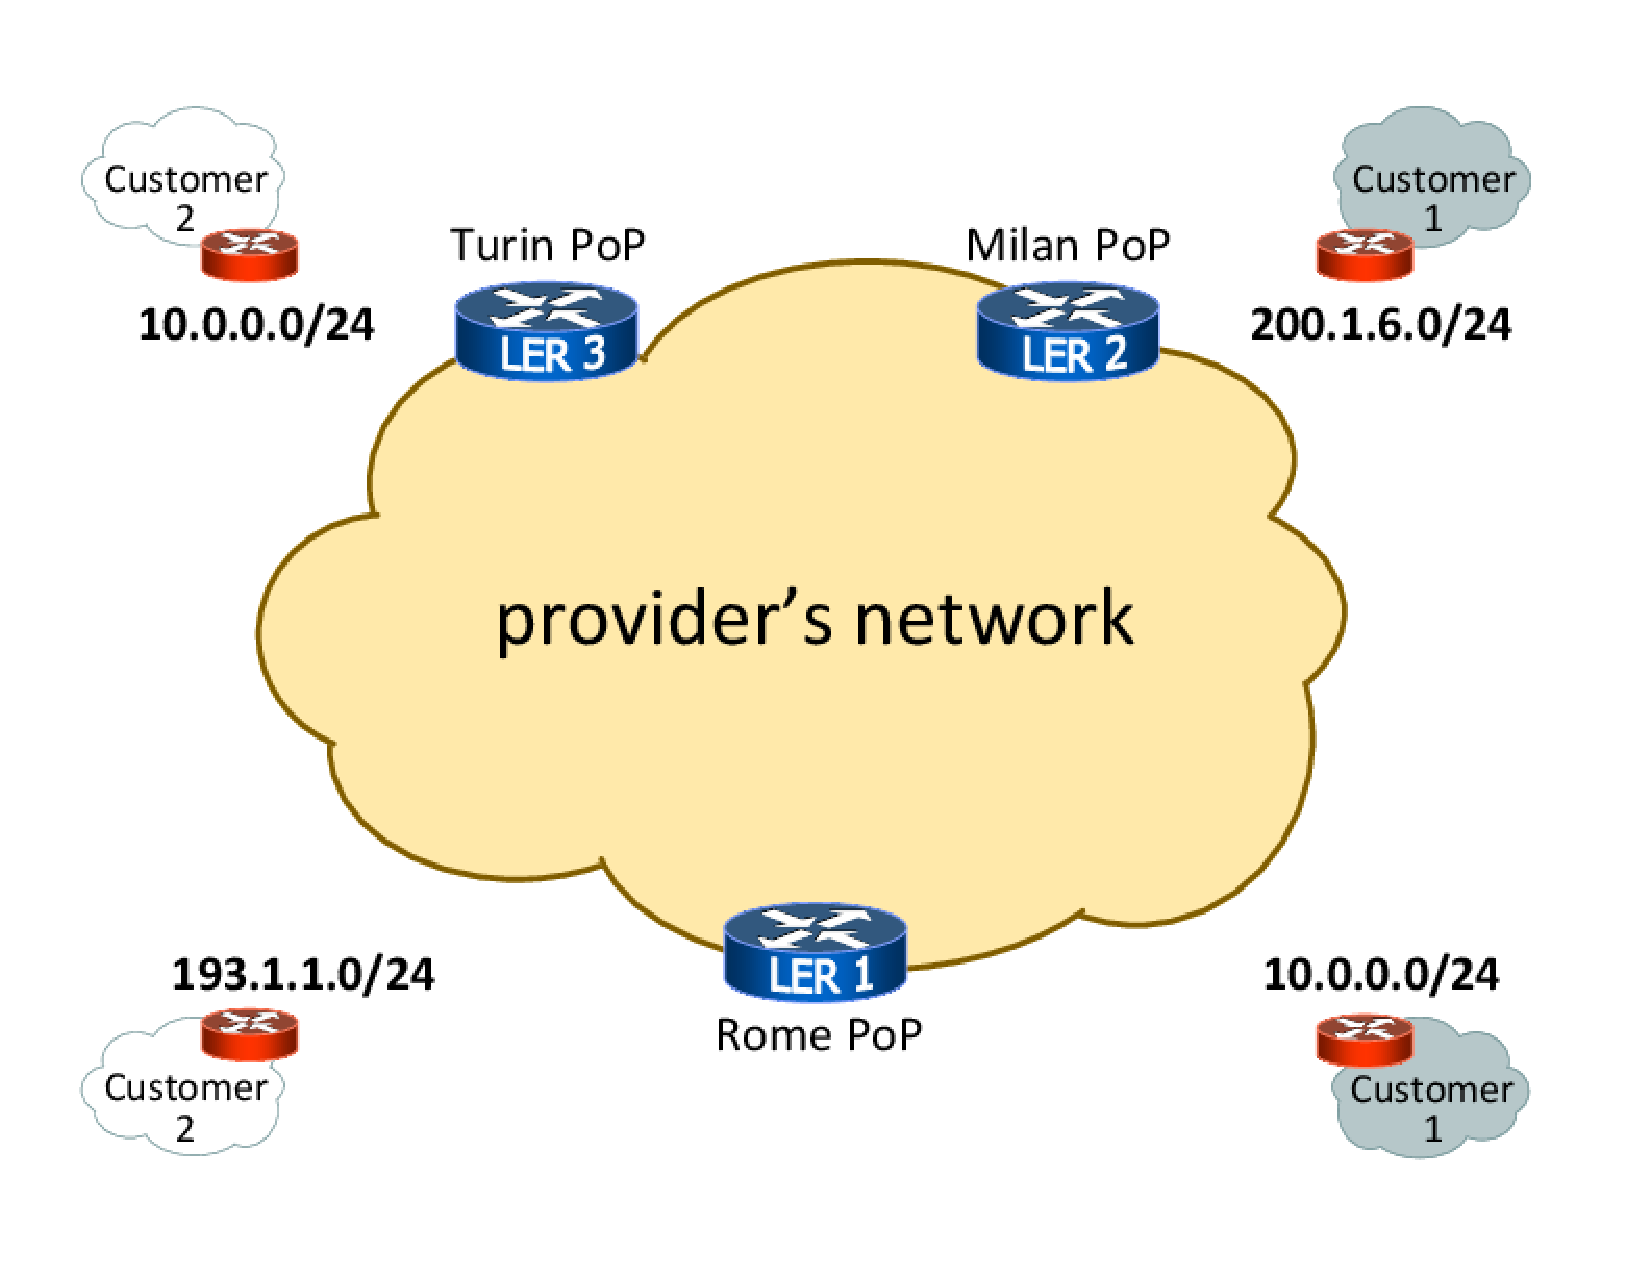
\includegraphics[trim=0cm 1cm 0cm 3cm, clip=true, width=0.7\columnwidth]{figures/mpls-slides-0}}
 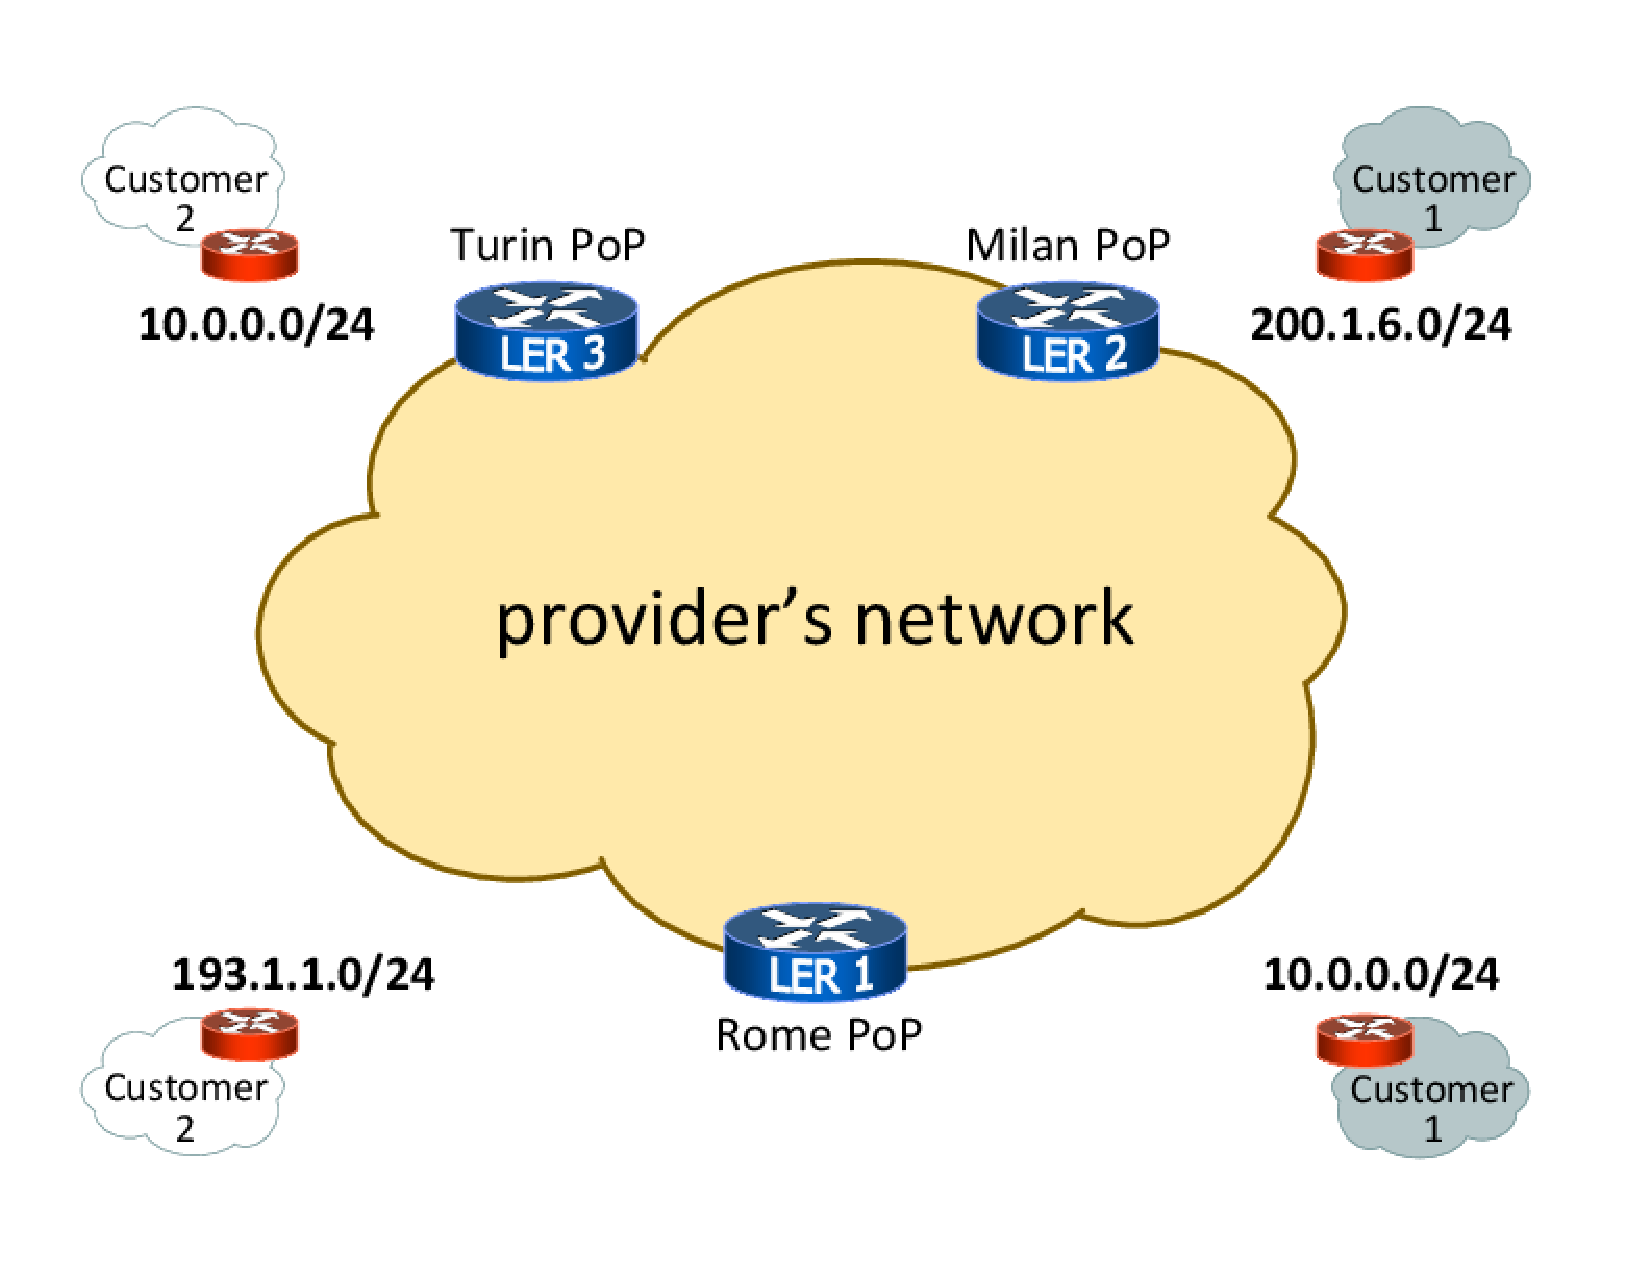
\includegraphics[trim=0cm 1.5cm 0cm 1.5cm, clip=true, width=0.7\columnwidth]{figures/mpls-slides-0}
 \caption{The sample network used throughout this chapter.}
 \label{fig:mpls-slides-0}
\end{figure}


\begin{shaded}
\noindent
Throughout this chapter we will refer to a very simple scenario (see
Fig.~\ref{fig:mpls-slides-0}) where a provider has a network infrastructure with three
PoPs (in Turin, Milan, and Rome) and offers connectivity to two customers. Customer 1 has
two sites and has an IP addressing plan that allocates the $200.1.6.0/24$ to its site
in Milan and the $10.0.0.0/24$ to its site in Rome. Customer 2 has two sites too
and has an IP addressing plan that allocates the $10.0.0.0/24$ to its site in Turin
and the $193.1.1.0/24$ to its site in Rome. Observe that the two customers have overlapping IP address space.

We will use the sample scenario to illustrate most of the concepts introduced in 
this chapter. The text that describes and refers to the sample scenario will be 
framed into shaded boxes like the one that encloses this paragraph. The configuration
language is that of a leading router vendor and references can be found
in~\cite{de-ghein}.
\end{shaded}
%%%%%%%%%
%%%%%%%%%
%%%%%%%%%
%%%%%%%%%
\section{Background and Terminology}\label{se:background}

In this section we introduce the reader to basic concept and terminology about 
Label Switching (also known as Label Swapping) and Virtual Private Networks.

Throughout the chapter, we extensively refer to two tightly related yet 
distinct concepts: forwarding and routing. \emph{Forwarding} is the process of receiving 
a packet from a network interface and deciding on which interface that packet 
should be sent. Usually, in order to minimize the latency of traversing a 
router, the decision about where to forward a packet is taken based on some 
pre-computed data structure. 
This is usually referred to as the \emph{forwarding table} because a table is 
the simplest logical structure to accommodate forwarding information. A table 
can be used as a physical data structure if addresses can be matched exactly. 
However, IP addresses must be forwarded based on the longest matching 
prefix~\cite{rfc4632}. This implies that efficient IP lookups need a more 
sophisticated data structure than a table. We refer the reader 
to~\cite{varghese} for a discussion on various data structures and algorithms to 
speed up prefix-match lookups, which exceeds the scope of this chapter. In the 
following, we simply refer to the logical forwarding table, irrespective of the 
actual physical data structure.

\emph{Routing} is the process by which each router builds its forwarding table 
and adapts it as the network topology changes over time.

Correspondingly, we have \emph{forwarding and routing protocols}, where the 
formers describe the formatting rules for network packets and the conventions 
that routers and hosts have to follow in order to exchange them, while the 
latter describe packet formats and conventions used to exchange routing 
information among routers. The information that routing protocols provide is 
used by each router to populate its forwarding table.

Finally, standard network terminology distinguishes between the corresponding 
router's software layers. Namely, the layer where the forwarding process takes 
place is called \emph{data plane} or \emph{forwarding plane}, while the layer 
where the routing process is managed is called \emph{control plane}.

%
%%%
%%%%%
%%%
%
\subsection{Label Switching}
In this section we introduce the concept of label switching as a 
forwarding paradigm. After having described the fundamentals characteristics of 
label switching in general, we move to MPLS-specific details in the following 
sections.
Traditionally, there are two different approaches to packet forwarding, each mapping to a
specific structure of the forwarding table. They are called \emph{forwarding by network
address} and \emph{label switching}.

The most intuitive approach is \emph{forwarding by network address}, that is the 
approach of IP. When a packet arrives at a router, the router parses the 
destination address from the packet header and looks it up in its forwarding 
table. The forwarding table has a simple 2-column structure where each row maps 
a destination address to the egress interface that the packet should be 
forwarded to (see Table~\ref{tab:fib-destination}). For scalability and 
efficiency reasons, it is possible to aggregate several destination prefixes 
into a single row, provided that they can be numerically aggregated and that 
they share the same egress interface.

\begin{table}
 \centering
 \begin{tabular}{|c|c|}
 \hline
 \textbf{Destination address} & \textbf{Egress interface} \\
 \hline
 10.100.100.0/24 & en2 \\
 \hline
 10.100.200.128/25 & en1 \\
 \hline  
 22.30.100.0/24 & en2 \\
 \hline \end{tabular}
 \caption{Structure of the forwarding table in the ``forwarding by network 
address'' approach.}
 \label{tab:fib-destination}
\end{table}

An alternative approach is known as \emph{label switching}\remove{, that is the approach of MPLS}. 
Essentially, while forwarding by network address requires that the egress 
interface be chosen based on the \emph{destination} of the packet, label 
switching requires that such an interface be chosen based on the \emph{flow} 
the packet belongs to, where a flow corresponds to an instance of transmission, i.e., a set of
packets, from a source to a destination and is identified by a tag (called \emph{label})
attached to each packet of the flow.

\begin{figure}
\centering  % left bottom right top
 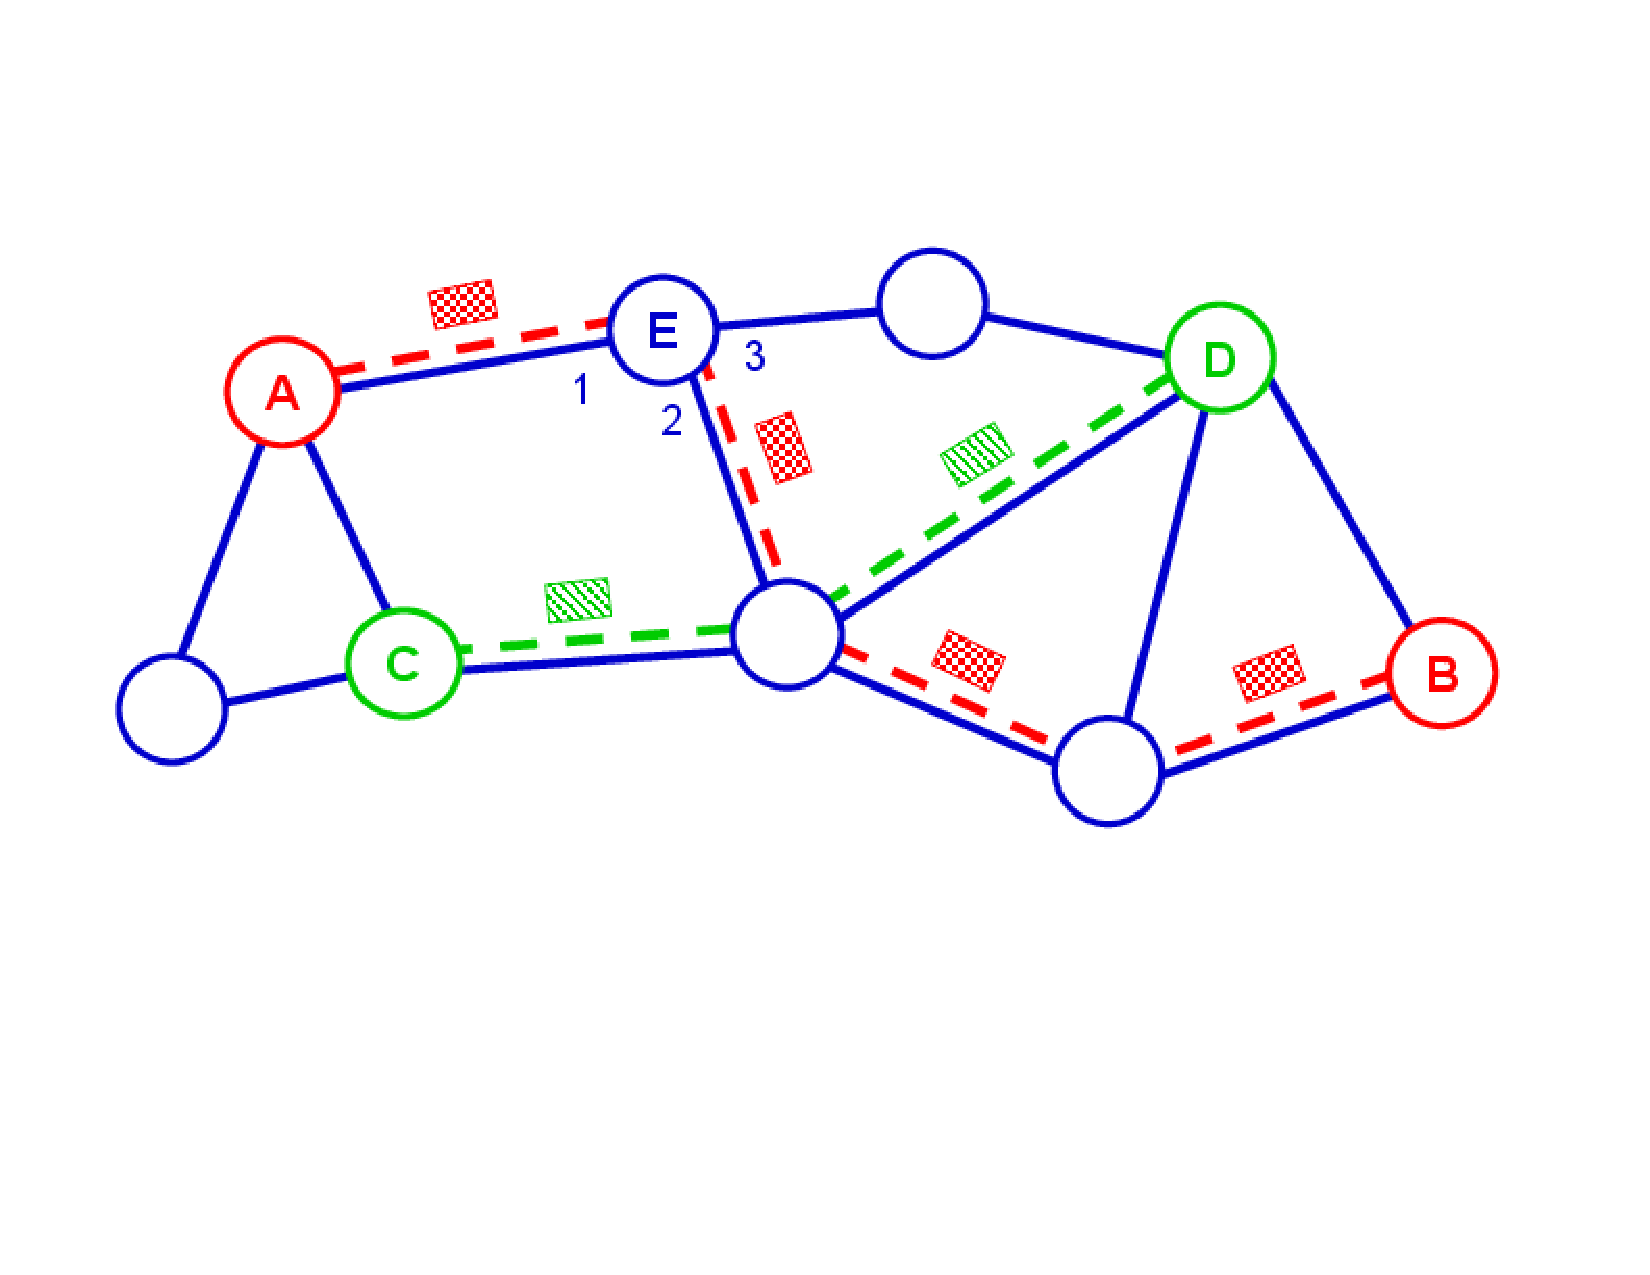
\includegraphics[trim=1cm 7cm 2cm 4cm, clip=true,width=0.7\columnwidth]{figures/reti-slides-0}
% \frame{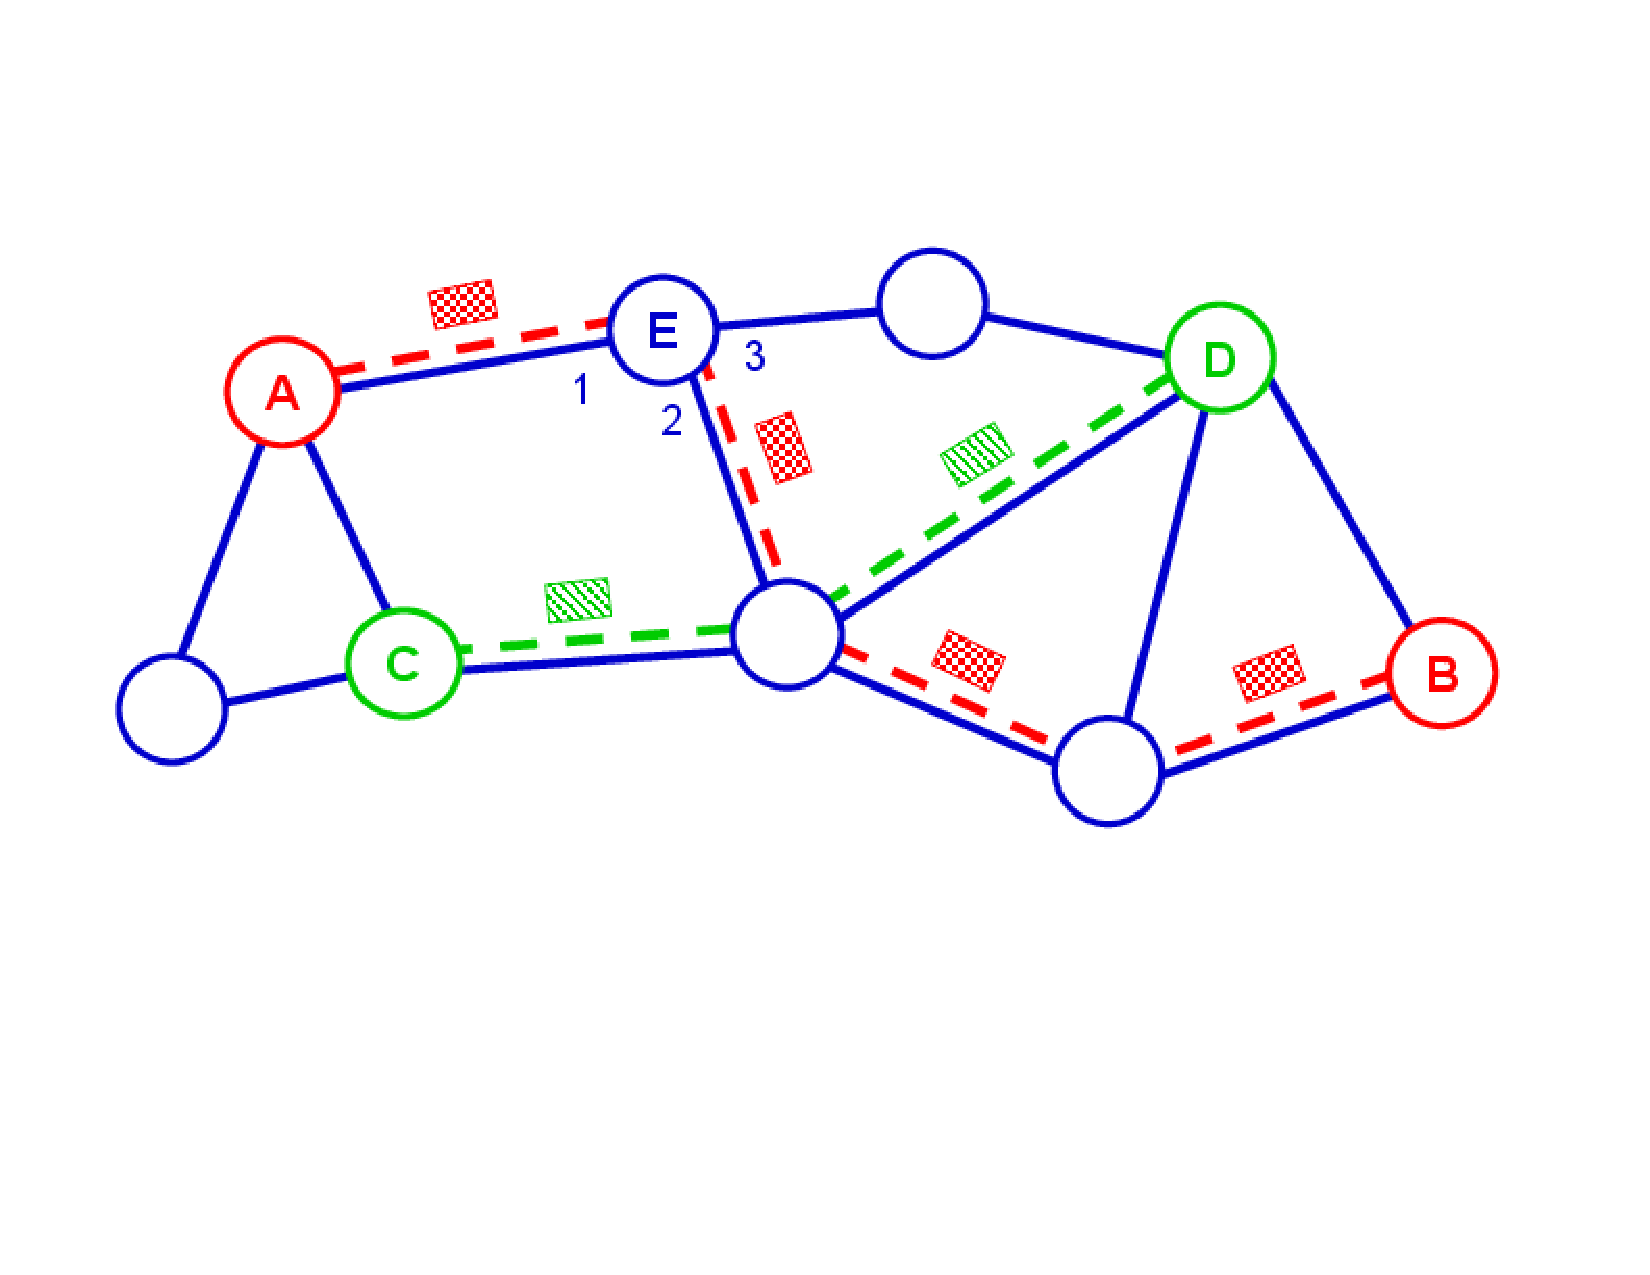
\includegraphics[trim=1cm 7cm 2cm 4cm, clip=true,width=0.7\columnwidth]{figures/reti-slides-0}}
 \caption{A label switching network (where labels are not swapped at each hop).}
 \label{fig:reti-slides-0}
\end{figure}


\begin{figure}
\centering
 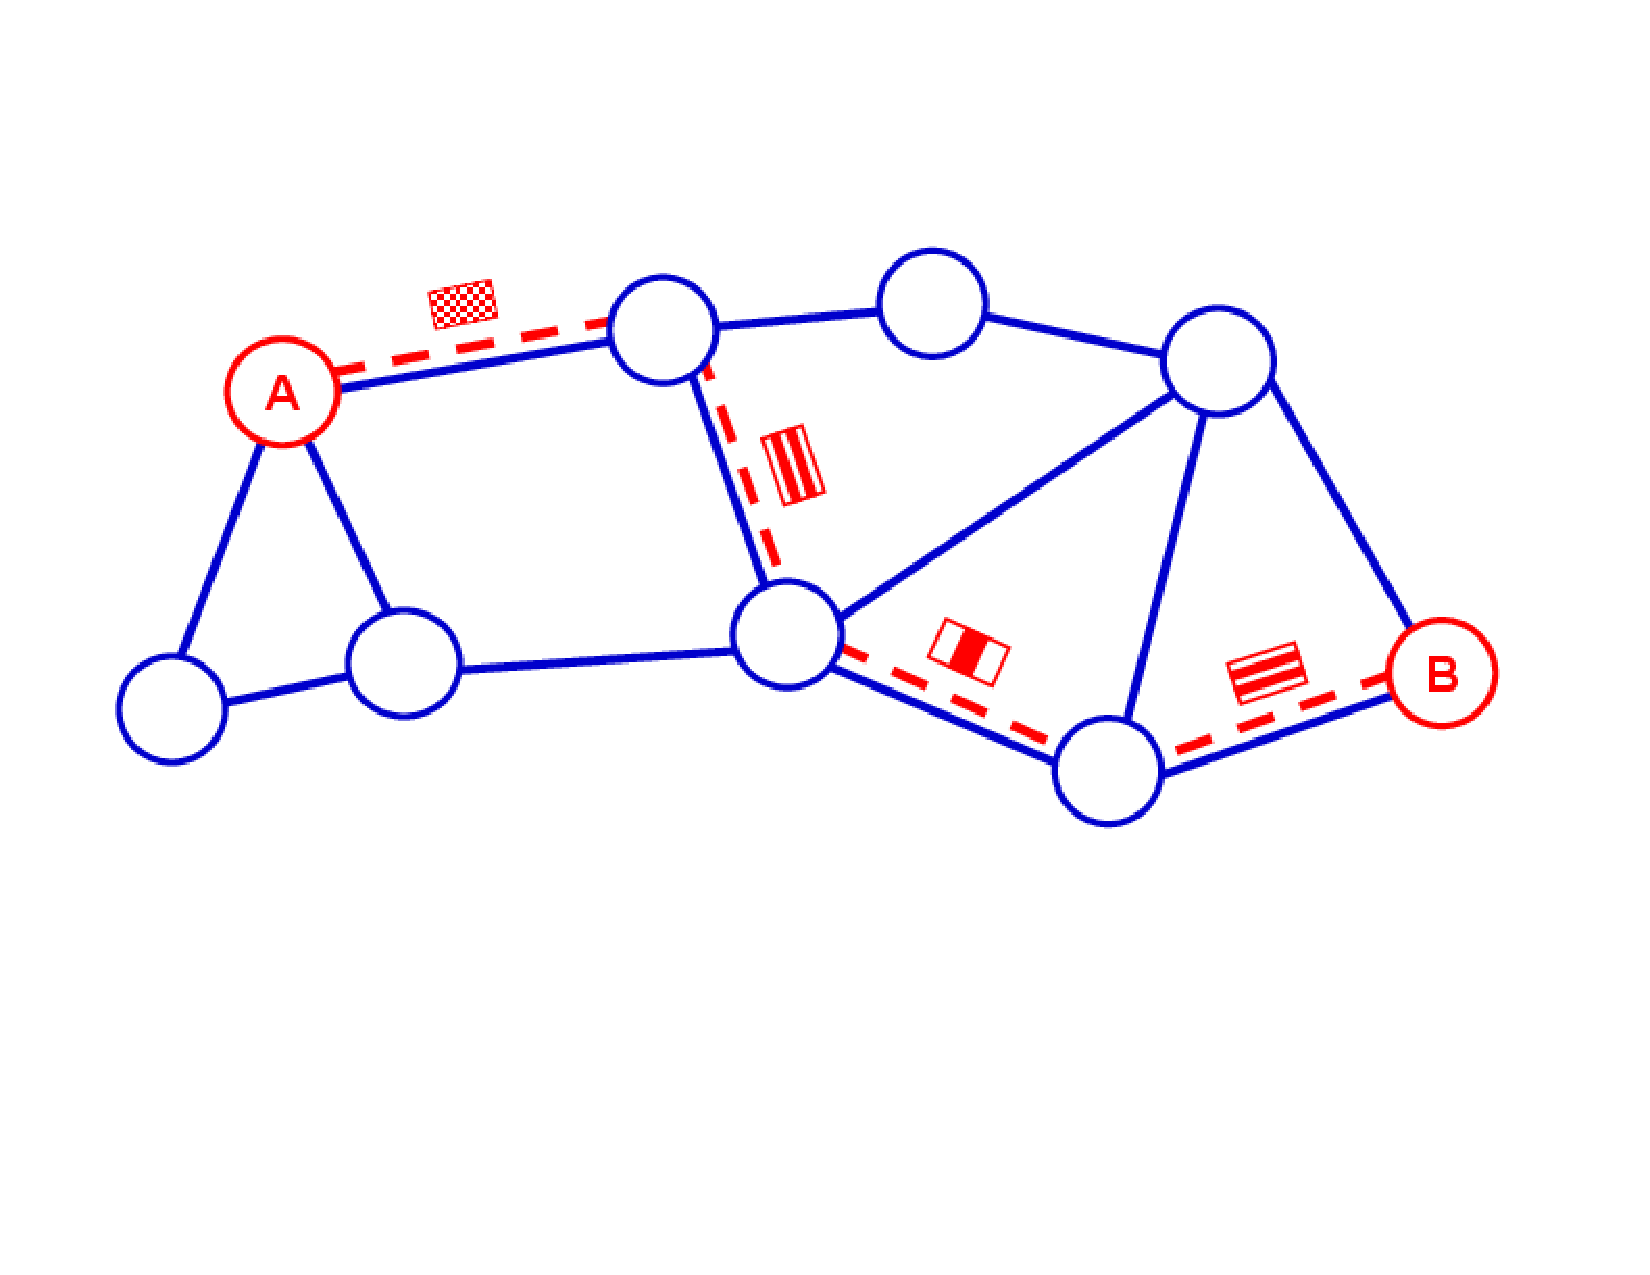
\includegraphics[trim=1cm 7cm 2cm 4cm, clip=true,width=0.7\columnwidth]{figures/reti-slides-1}
 \caption{A label switching network (where labels are swapped at each hop).}
 \label{fig:reti-slides-1}
\end{figure}




\begin{table}
 \centering
 \begin{tabular}{|c|c|c|c|}
 \hline
 \textbf{Incoming interface} & \textbf{Incoming label} & \textbf{Egress 
interface} &  \textbf{Egress label} \\
 \hline
 en2 & 101 & en5 & 218 \\
 \hline
 \end{tabular}
 \caption{Structure of the forwarding table in the ``forwarding by label 
swapping'' approach with per-interface label scope.}
 \label{tab:fib-label-interface}
\end{table}

\begin{table}
 \centering
 \begin{tabular}{|c|c|c|}
 \hline
 \textbf{Incoming label} & \textbf{Egress interface} &  \textbf{Egress label} \\
 \hline
 101 & en5 & 218 \\
 \hline
 \end{tabular}
 \caption{Structure of the forwarding table in the ``forwarding by label 
swapping'' approach with per-router label scope.}
 \label{tab:fib-label-router}
\end{table}

As an example, Fig.~\ref{fig:reti-slides-0} shows a label switching network 
where each flow has an associated label (labels are represented with colors). 
Packets with a red label belong to the flow from router A to router B of Fig.~\ref{fig:reti-slides-0}.
If a packet with a red label enters interface 1 of router E, it will exit from interface 2 with the same label.

If the label switching technologies 
followed the approach of Fig.~\ref{fig:reti-slides-0} they would have the 
advantage that labels do not have to be changed at each hop. On the other hand, if they 
did they would have the big drawback of 
requiring a centralized control of the assigned labels, as labels should be unique for the entire network. 
Fig.~\ref{fig:reti-slides-1} shows what actually happens in label switching 
networks, where labels are swapped at each hop. This choice requires that labels 
are unique for each router or for each interface only and does not need a 
centralized control. Fig.~\ref{fig:reti-slides-2} illustrates the forwarding 
table of a router. Independent of whether labels are swapped at 
each hop or not, the forwarding paths towards the same destination node 
typically form a tree rooted at the destination node itself, even though this is 
not mandatory.

More formally, the operations performed by a label switching router can be summarized as follows.
When the packet arrives at the router, the router extracts (\emph{pops}) the label 
from the header, looks the label value up in its forwarding table, and finds
\begin{inparaenum}[(i)]
 \item the egress interface the packet should be forwarded to, and
 \item a new label to apply (\emph{push}) to the packet.
\end{inparaenum}

A forwarding process based on labels rather than destination addresses poses 
challenges to the corresponding routing protocols. In fact, the instances of 
flow traversing the network might be much more volatile than the addressing scheme 
used to identify their destinations. Before transmitting a new flow, a route 
from its source to its destination has to be computed and a new label has to be 
assigned to each leg of the route. As observed before, in order to facilitate the task of
picking a 
new, unused, label, labels are not required to be unique for the entire network but are
required to be unique for each router or for 
each interface only. This is why they have to be changed at each hop.      %
Depending on whether labels have a per-interface or per-router scope, the 
forwarding table is structured as in Table~\ref{tab:fib-label-interface} or 
Table~\ref{tab:fib-label-router}, respectively. 
Observe that such a simple structure for forwarding tables 
allows efficient lookups (e.g., by using a hash table or a direct access table).


Label switching is not a unique feature of MPLS and it is not necessarily 
implemented at the network level of the protocol stack: other protocols, notably 
ATM and Frame Relay, traditionally adopt the same forwarding mechanism. 
Initially, the reason to prefer label switching was performance: looking up a 
label value in the forwarding table was much faster than looking up an IP 
address. Besides the fact that labels can take values in a much smaller range 
than IP addresses, label values can be looked up exactly, while IP addresses 
need to be looked up by the longest matching prefix. However, modern routers use 
extremely specialized hardware (e.g., content-addressable memories) and very 
efficient data structures (e.g., tries) to implement their forwarding tables, in 
such a way that the performance gain of label switching over forwarding by 
destination address is now believed to be no longer an argument.

\begin{figure}
\centering
% 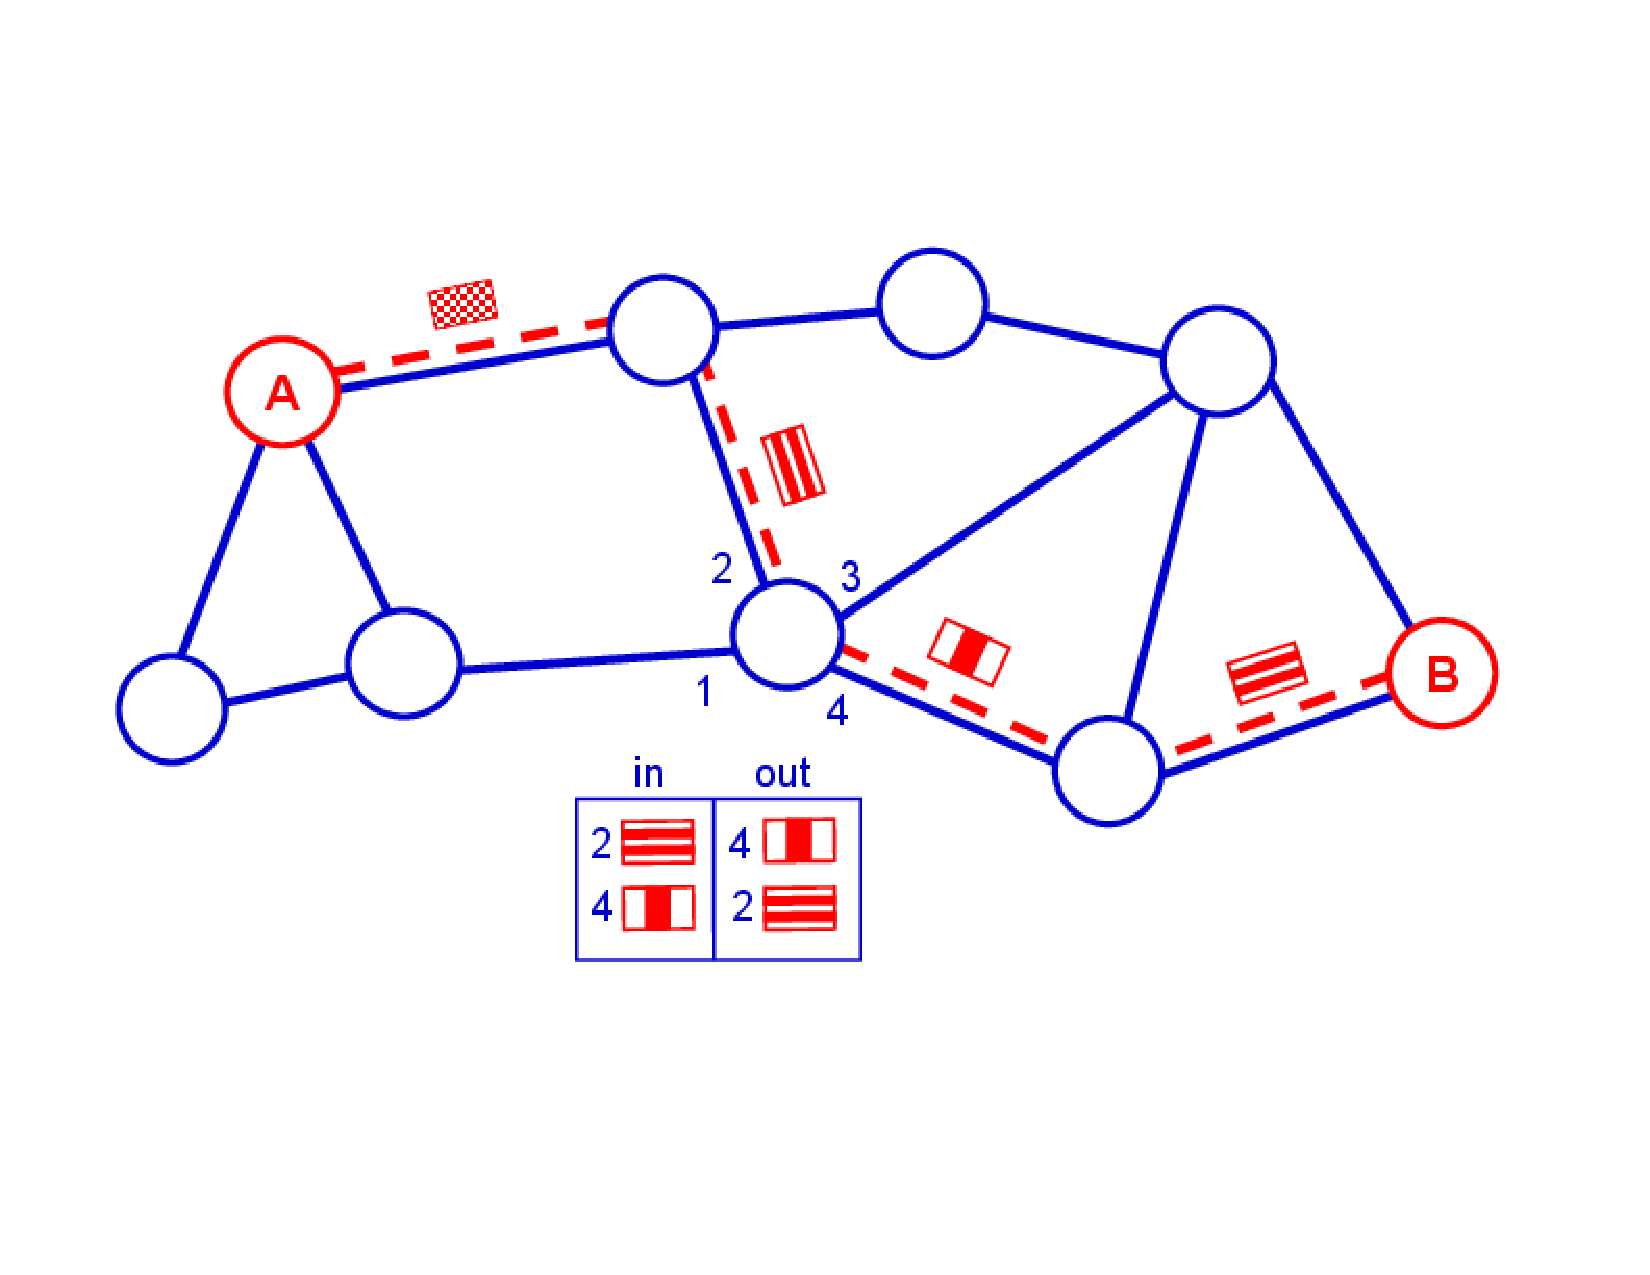
\includegraphics[width=0.7\columnwidth]{figures/reti-slides-2}
% left bottom right top
% \frame{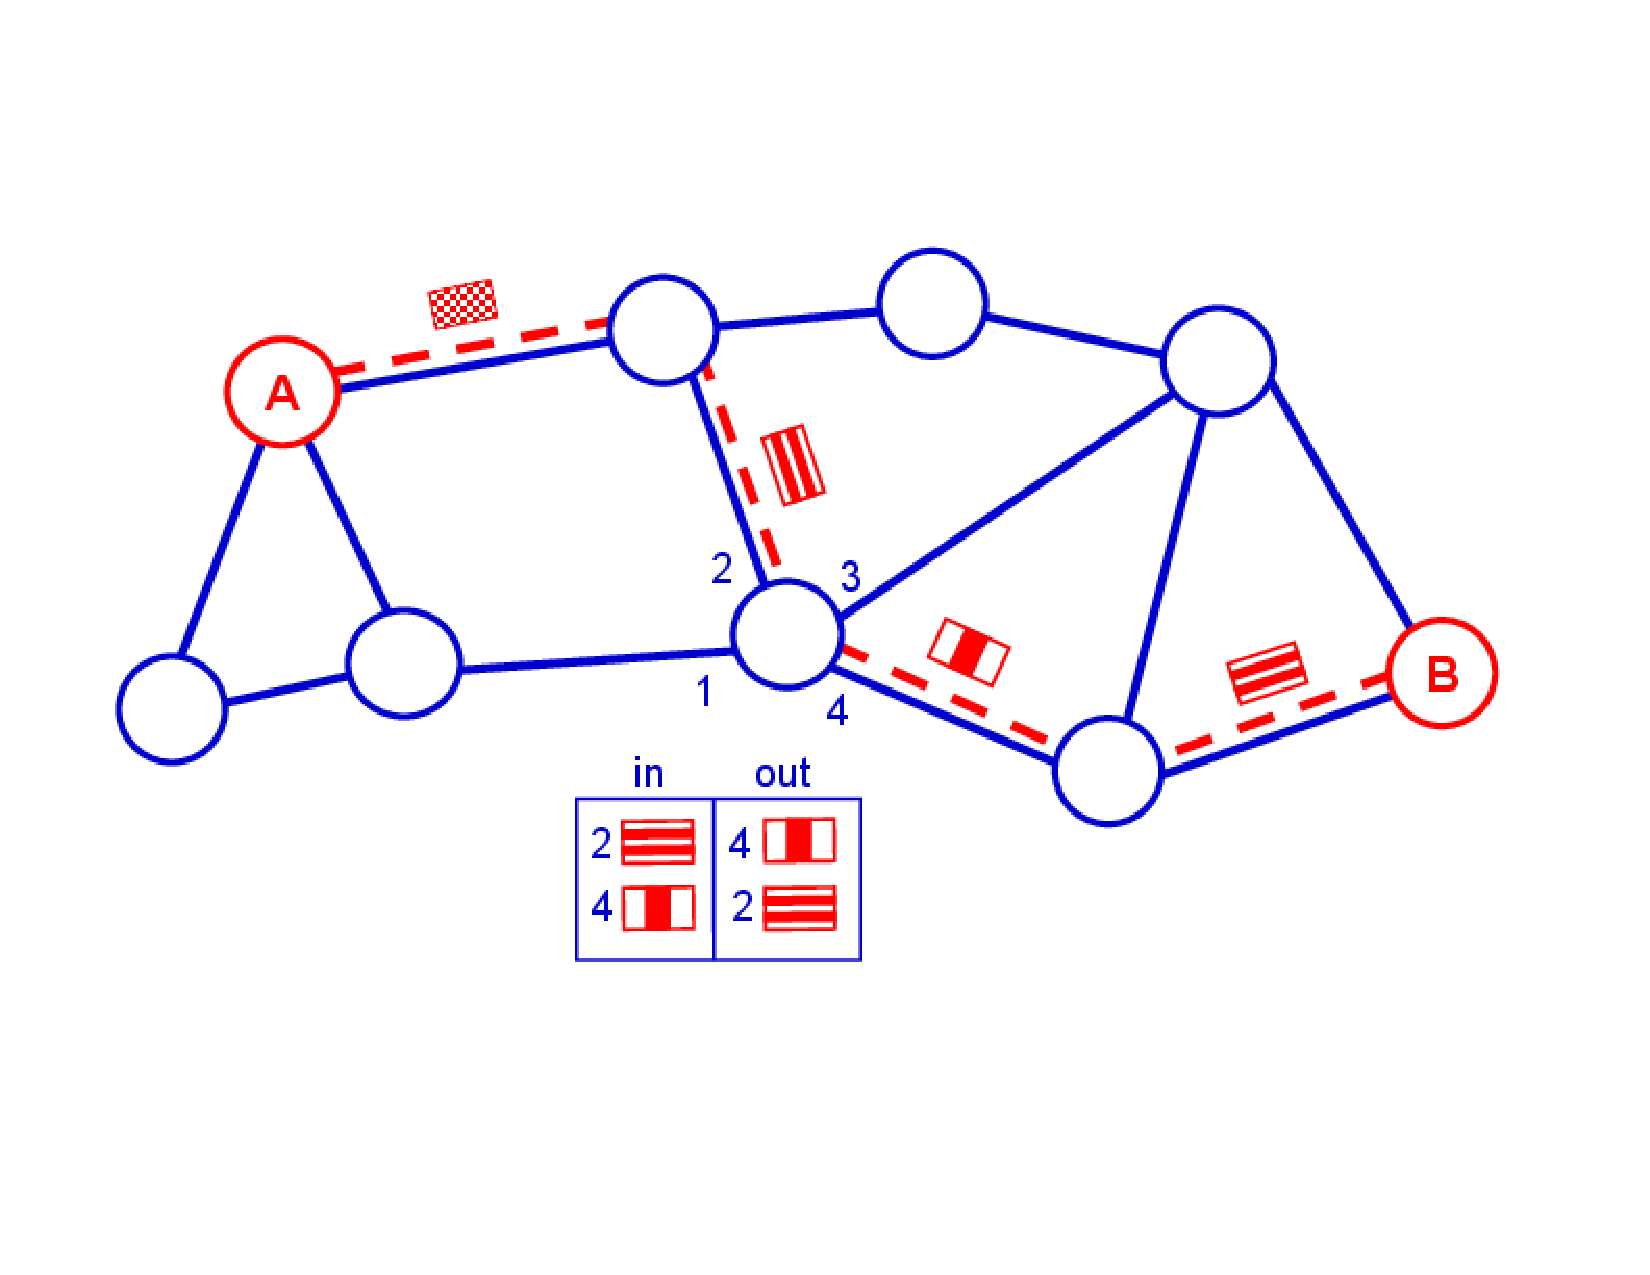
\includegraphics[trim=1cm 5cm 2cm 4cm, clip=true,width=0.7\columnwidth]{figures/reti-slides-2}}
 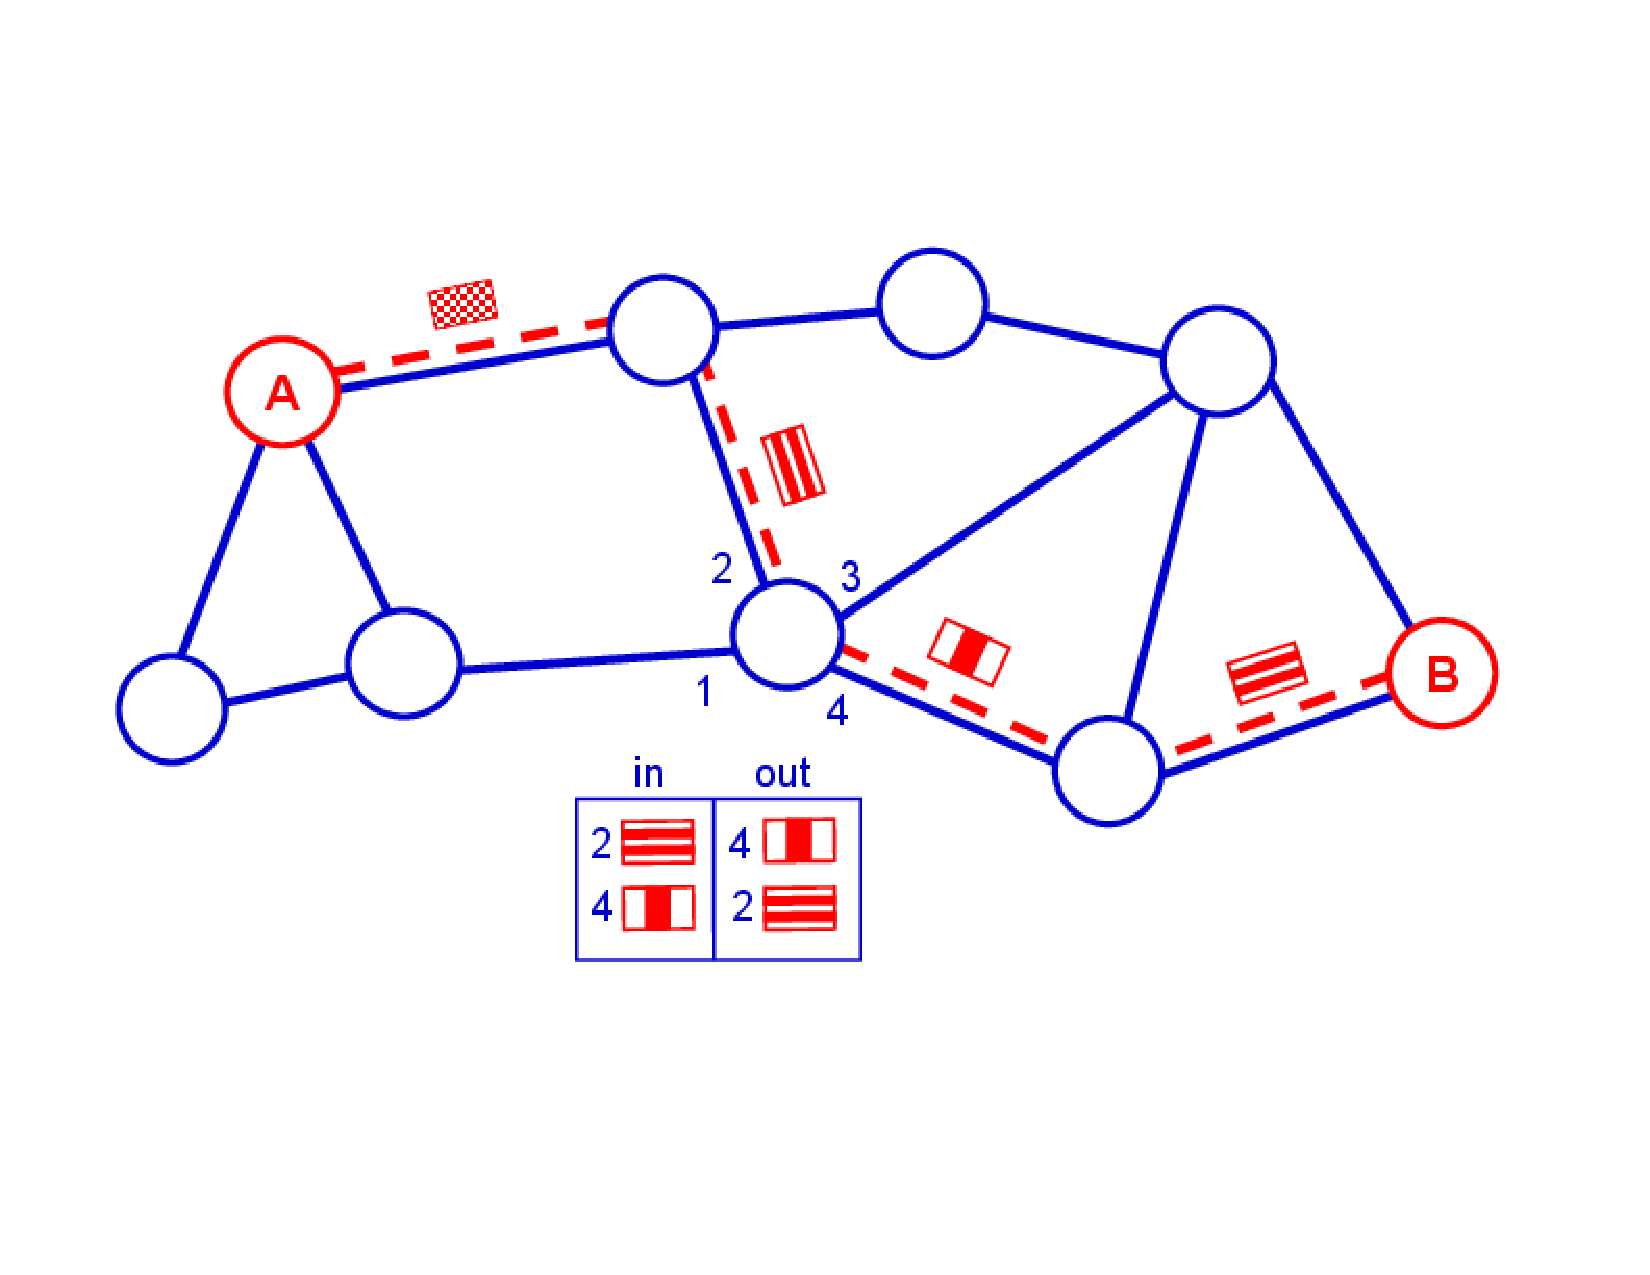
\includegraphics[trim=1cm 5cm 2cm 4cm, clip=true,width=0.7\columnwidth]{figures/reti-slides-2}
 \caption{A label switching network where the forwarding table of a router is shown.}
 \label{fig:reti-slides-2}
\end{figure}


% A few points have to be observed with respect to the relationship among a label 
% switching protocol and other protocols of the same network:
% \begin{itemize}
% 
% \item While, in theory, it would be possibile to fill in forwarding tables 
% manually, any practical use of the label switching approach computes them 
% automatically. The easiest strategy is that of following, hop by hop, the 
% routes computed by some other network protocol, usually with a forwarding by 
% destination address approach. This is why a label switching protocol usually 
% does not replace more traditional protocols, but rather relies on them. MPLS, 
% for example, uses IP routing tables to compute a route from source to 
% destination. 
% \item Traffic in a label switching network may be heterogeneous: labeled and 
% non-labeled packets may be received at the interfaces and forwarded based on 
% their first header. This is particularly important in view of the previous 
% observation. 
%Hence, when the header containing the label is placed directly 
% after the level 2 packet, as it is the case for MPLS, from the point of view 
% of 
% the forwarding process it may be considered as an alternative network 
% protocol. 
% \end{itemize}

%
%%%
%%%%%
%%%
%
\subsection{MPLS header and terminology}

The MPLS protocol brings the label switching forwarding paradigm to the extreme,
managing, instead of a single label, a whole stack of labels, where the external one
determines the egress interface.
It does not fit the ISO/OSI model very well. The MPLS header is transported 
over L2 packets and can encapsulate L3 packets as well as L2 packets. 
% However, it relies 
% on information from L3 to build the router's forwarding tables. 
Since MPLS does 
not fit the definition of either L2 protocols nor L3 protocols, it is frequently 
referred to as a ``layer 2.5'' protocol, emphasizing the fact that it requires 
L2 connectivity and can encapsulate IP packets.

\begin{figure}
 \centering
 \begin{tabular}{l |c|}
 \cline{2-2}
  Layer 3 & IP \\ \cline{2-2}
  Layer 2.5 & MPLS \\ \cline{2-2}
  Layer 2 & Ethernet, Frame relay, ATM, PPP, etc \\ \cline{2-2}
  Layer 1 & Physical layer \\ \cline{2-2}	
 \end{tabular}
 \caption{MPLS and ISO/OSI network layers.}
 \label{fig:mpls-iso-osi}
\end{figure}


When an IP packet from a 
router needs to be transported over an MPLS 
backbone, the first MPLS-enabled router in the network pushes an MPLS header in 
between the Ethernet header and the IP header. The resulting packet layout is 
depicted in Fig.~\ref{fig:mpls-iso-osi}. 

The MPLS header consists of a \emph{stack} of 4-byte records where each record 
has the following structure (depicted in Fig.~\ref{fig:mpls-header}): 
\begin{itemize}
 \item a \textbf{label} field (20 bits), which carries the label value;
 \item a \textbf{ToS} field (3 bits) which is used to discriminate different 
levels of quality of service (QoS) and to carry explicit congestion 
notifications (ECN);
 \item a \textbf{bottom-of-stack} field (1 bit) which is set to 1 when the 
record is the last record in the stack; and
 \item a \textbf{TTL} field (8 bits) which is decremented at each hop, 
similarly to the TTL field in the IP header.
\end{itemize}

\begin{figure}
 \centering
 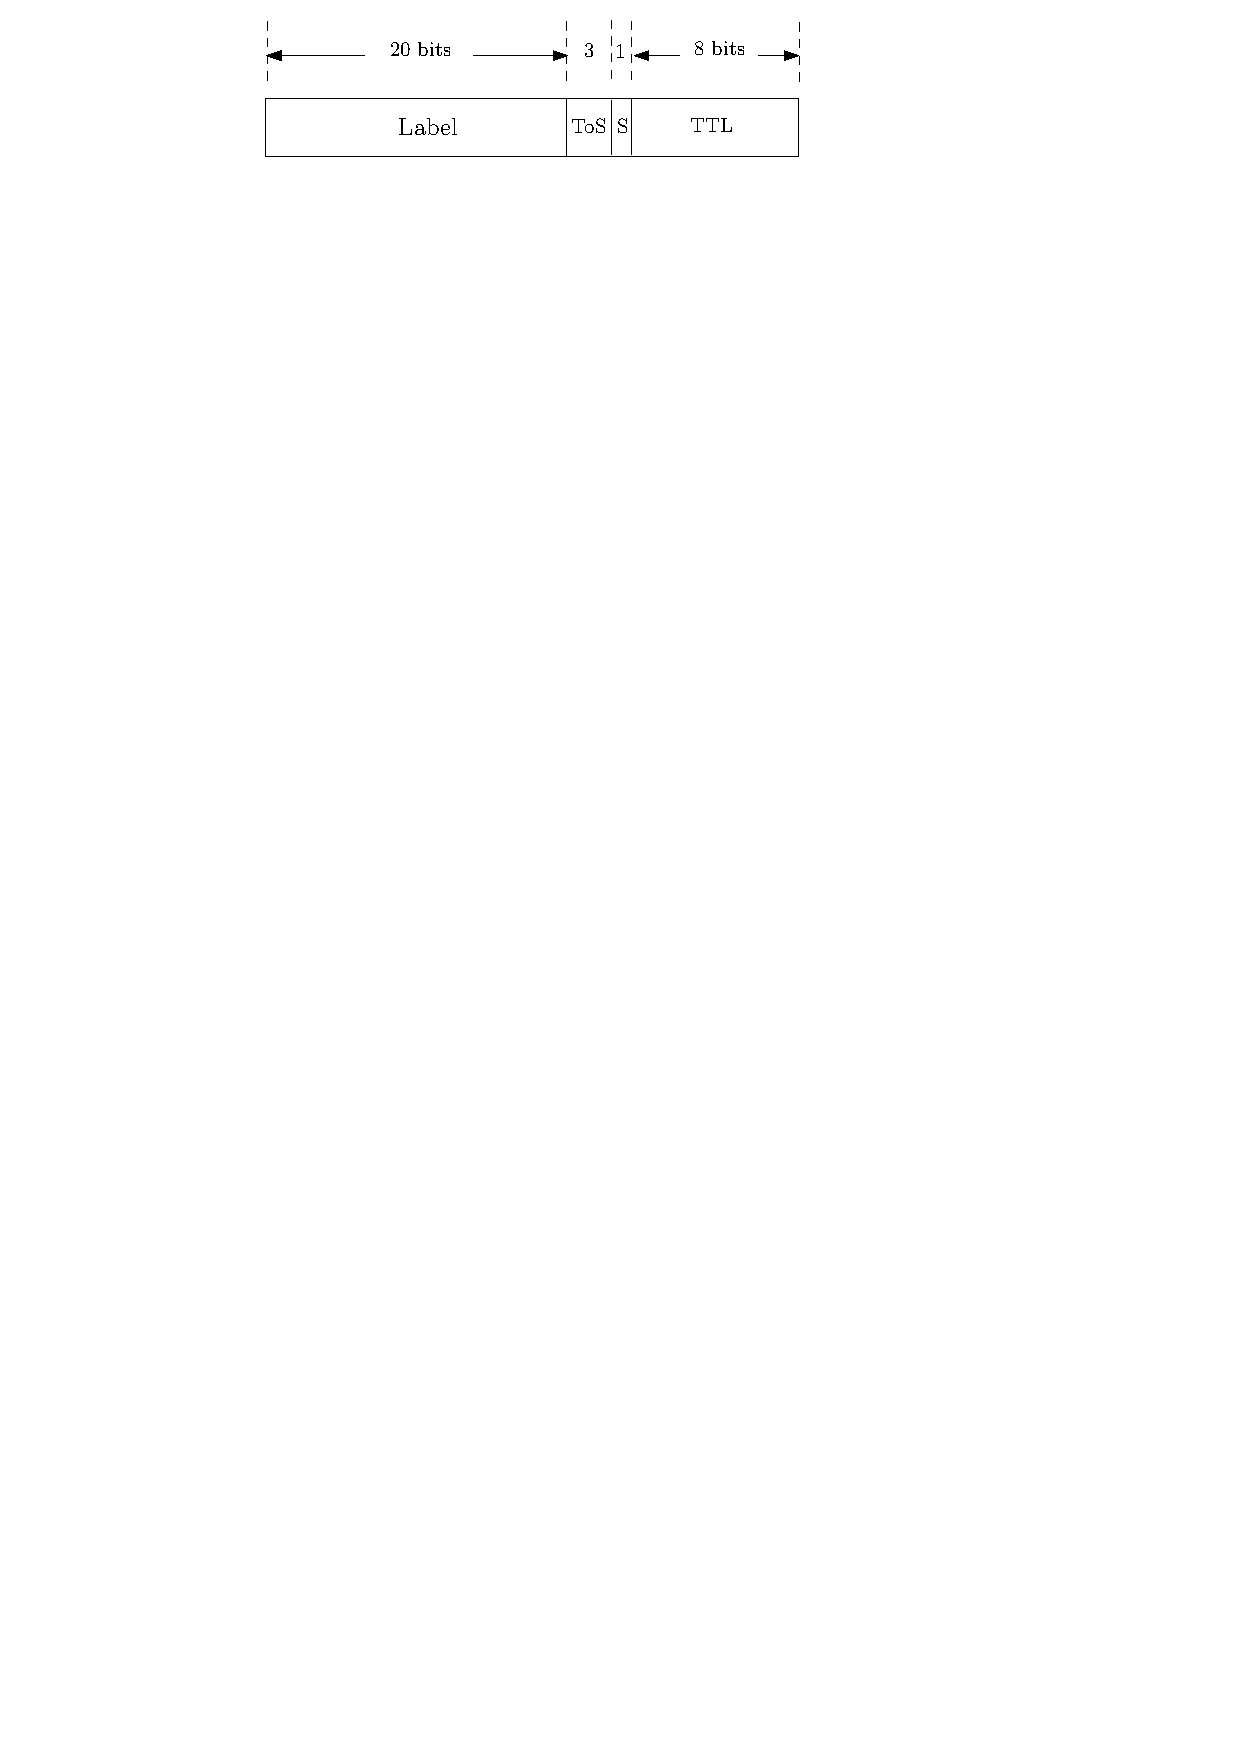
\includegraphics[width=0.7\columnwidth]{figures/mpls-header}
 \caption{Structure of a record in an MPLS header.}
 \label{fig:mpls-header}
\end{figure}

\begin{figure}[tb]
\centering
 %\frame{
 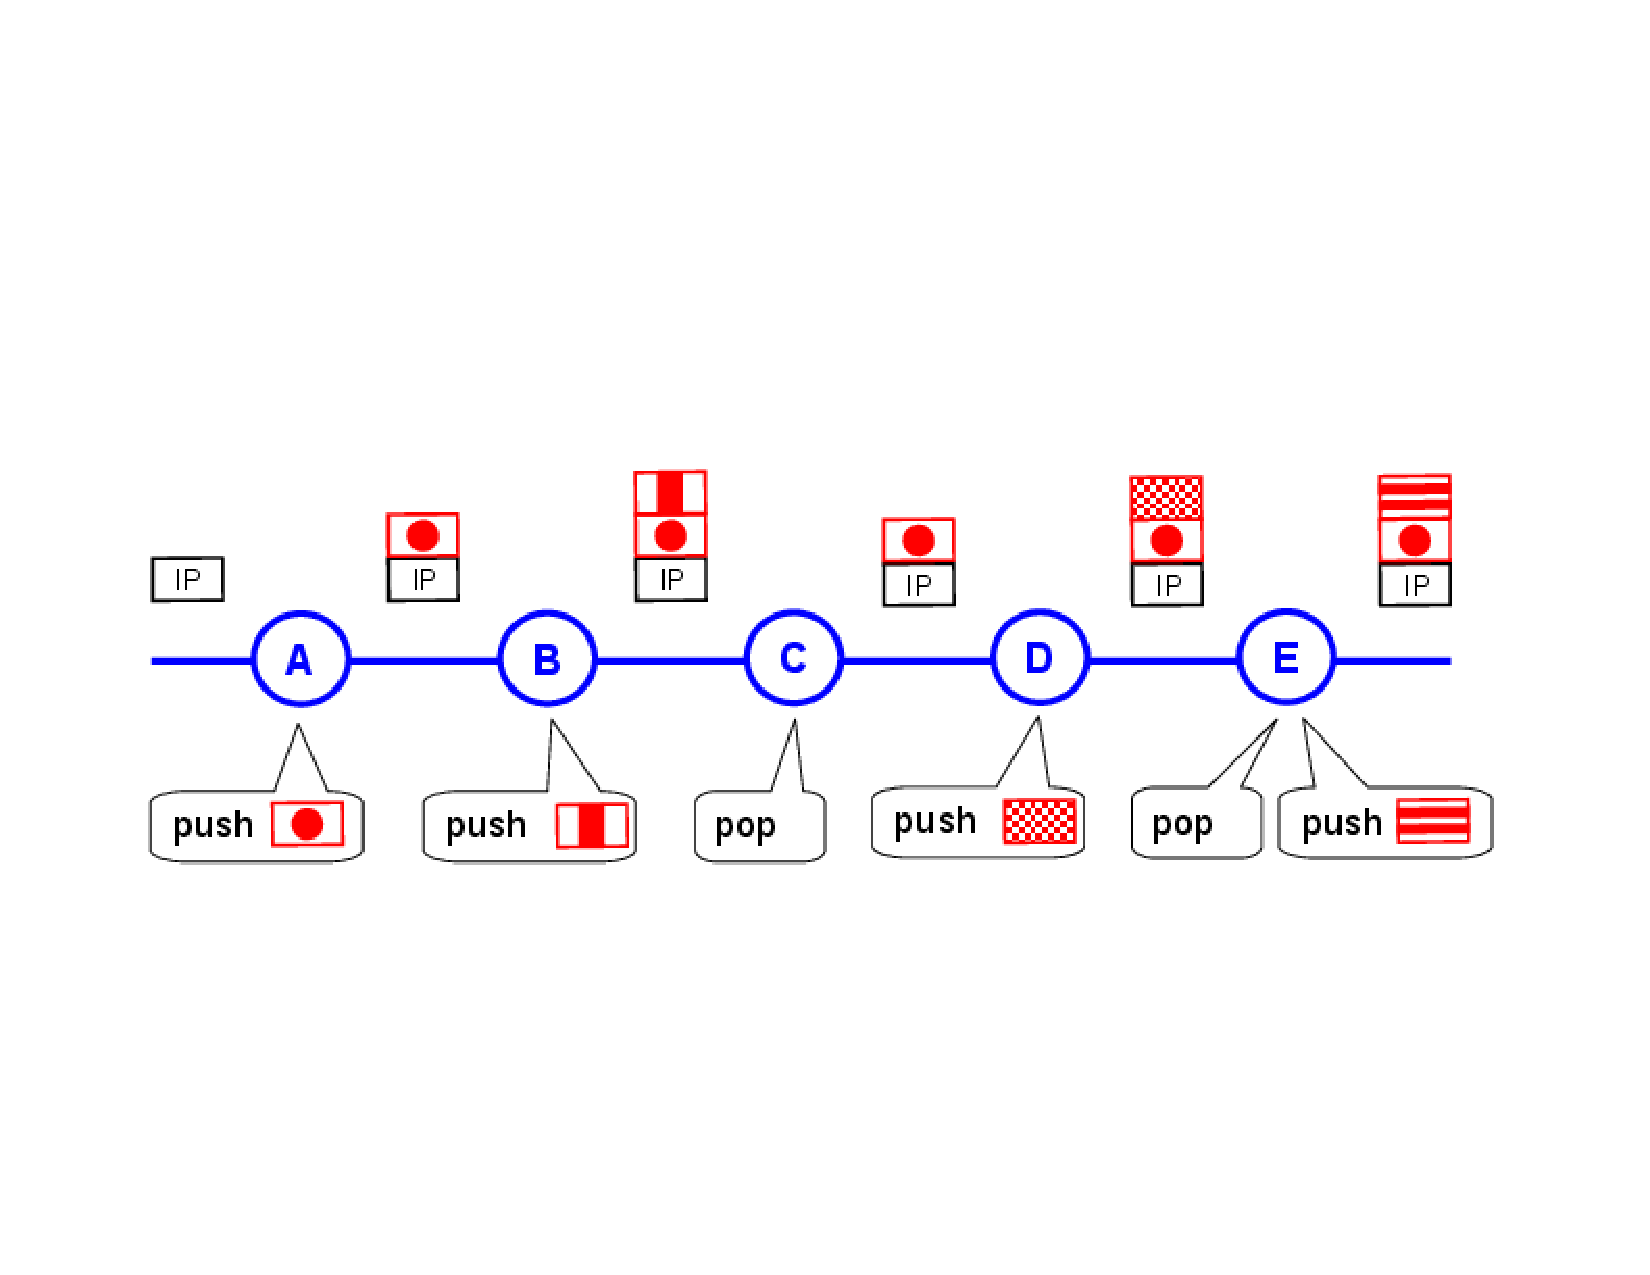
\includegraphics[trim=0cm 7cm 0cm 7cm, clip=true,
width=0.9\columnwidth]{figures/mpls-slides-28}
 %}
 \caption{The evolution of the MPLS label stack as a packet traverses several routers that perfom random push and pop operations.}
 \label{fig:mpls-slides-28}
\end{figure}


When an MPLS-enabled router receives a packet, it can perform three different 
operations:
\begin{inparaenum}[(i)]
 \item \emph{push} a label onto a (possibly empty) stack,
 \item \emph{pop} a label from the stack (possibly resulting in an empty 
stack), or
 \item \emph{swap} the top label of the stack, which can be seen as a pop 
operation followed by a push operation.
\end{inparaenum}
% 
Figure~\ref{fig:mpls-slides-28} shows the evolution of the MPLS label stack as a packet traverses several routers that perform  random push and pop operations.

MPLS-VPN terminology uses specific names to distinguish routers that do not understand 
labels at all, routers that push (or pop) labels, and routers that simply swap 
labels. 
%
Routers belonging to the first group are called \emph{customer edge} (CE) 
routers because they are not MPLS-enabled. Typically those are the customer's 
routers that need to be interconnected via an L3VPN. CE routers can only handle 
IP packets and are not aware of the MPLS layer which is used to implement the 
VPN.

Routers belonging to the second group are called \emph{provider edge} (PE) 
routers, or \emph{label edge routers} (LERs). They are placed at the edge of the 
MPLS backbone of the provider, have direct connectivity to the CE routers, and 
act as the access point for the customer to the VPN. While they need to perform label swap operations because they are part 
of the backbone, they spend most of their time pushing labels (when an IP packet 
comes from a CE router) and popping labels (when an MPLS packet needs to be 
forwarded to a CE router).

Routers belonging to the third group are called \emph{provider} (P) routers, or 
\emph{label switching routers} (LSRs). They are in the core of the MPLS network. 
Since they do not interact directly with non-MPLS routers, they mainly perform 
label swapping operations in order to forward packets to other P or PE routers.

MPLS groups destinations into Forwarding Equivalence Classes (FEC). 
Packets that need to be forwarded to the same CE using the same path and with 
the same quality of service belong to the same FEC.


\begin{figure}
\centering
 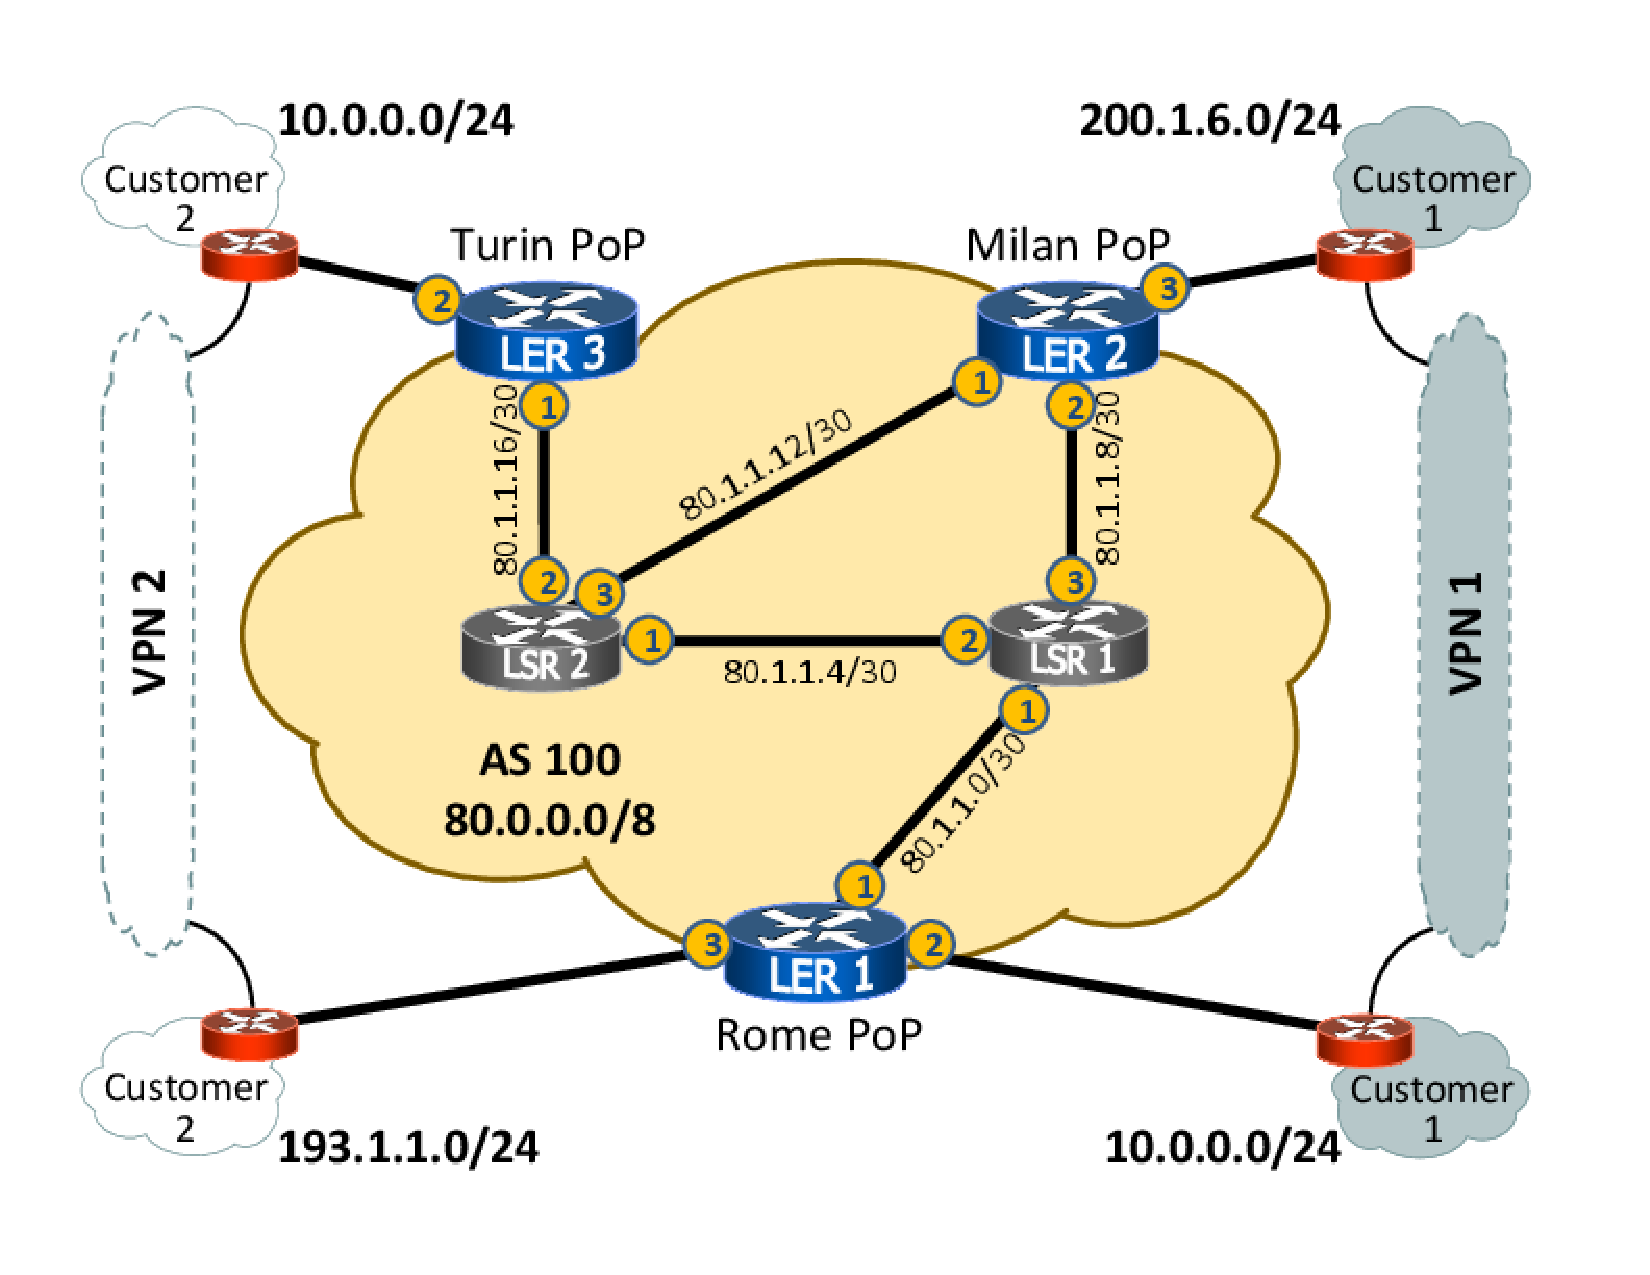
\includegraphics[trim=0cm 1.5cm 0cm 1.5cm, clip=true, width=0.7\columnwidth]{figures/mpls-slides-1}
 \caption{Inside the provider's infrastructure.}
 \label{fig:mpls-slides-1}
\end{figure}

% \begin{figure}
% \centering
%  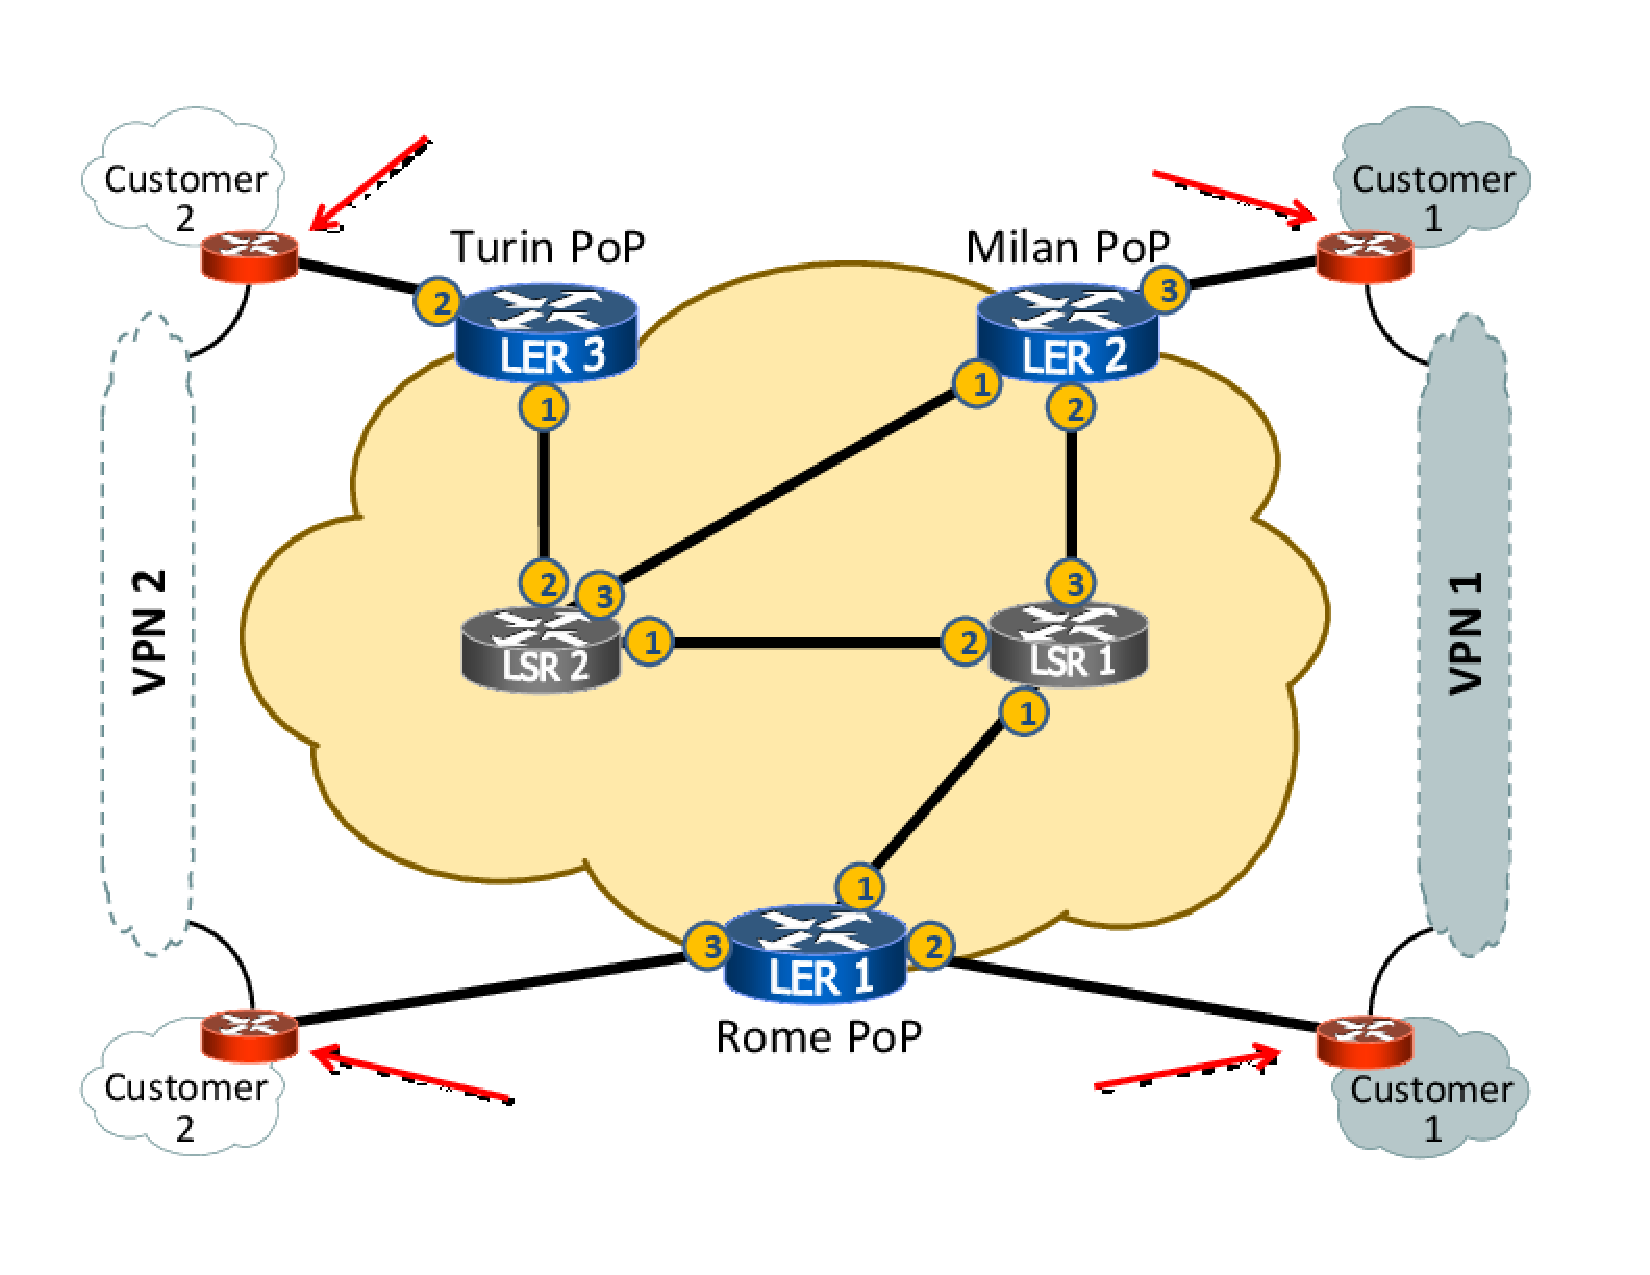
\includegraphics[width=0.7\columnwidth]{figures/mpls-slides-2}
%  \caption{CE -- Customer Edge Routers.}
%  \label{fig:mpls-slides-2}
% \end{figure}
% 
% \begin{figure}
% \centering
%  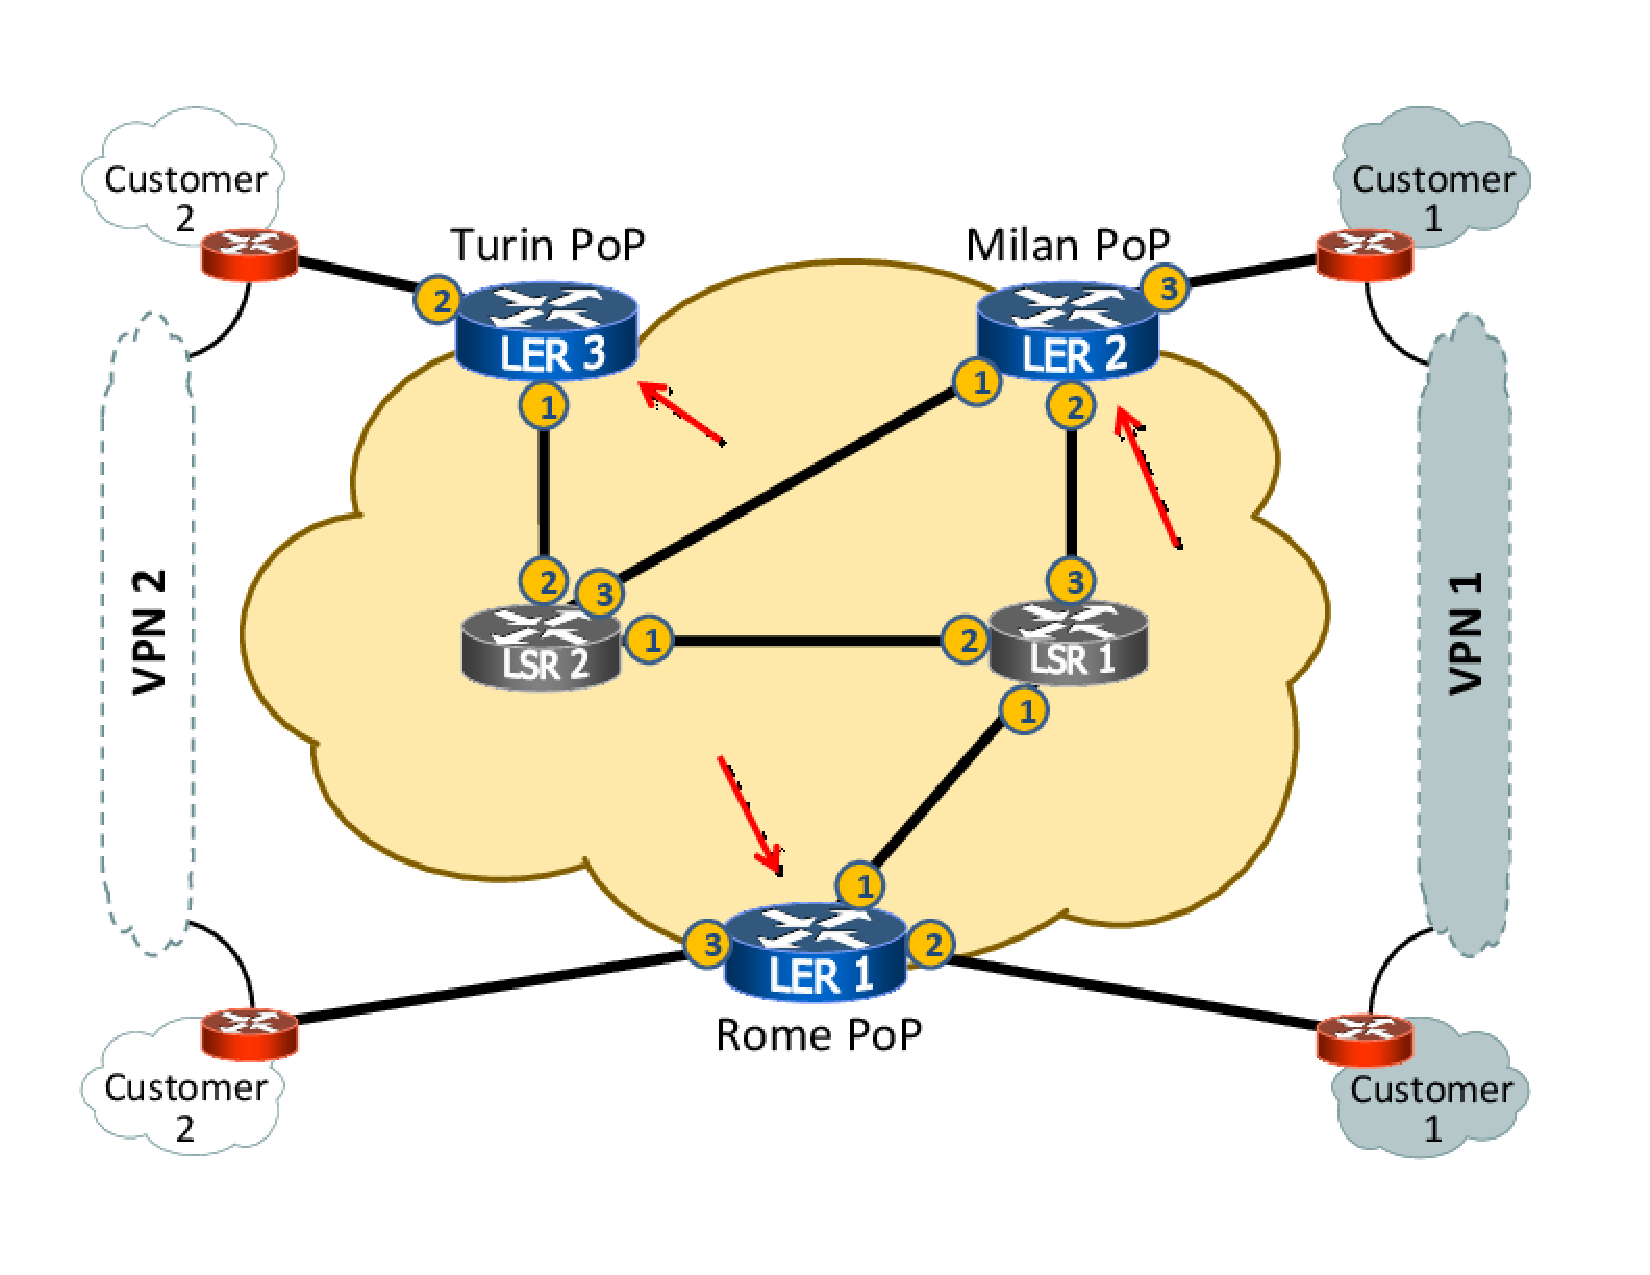
\includegraphics[width=0.7\columnwidth]{figures/mpls-slides-3}
%  \caption{PE -- Provider Edge Routers.}
%  \label{fig:mpls-slides-3}
% \end{figure}
% 
% \begin{figure}
% \centering
%  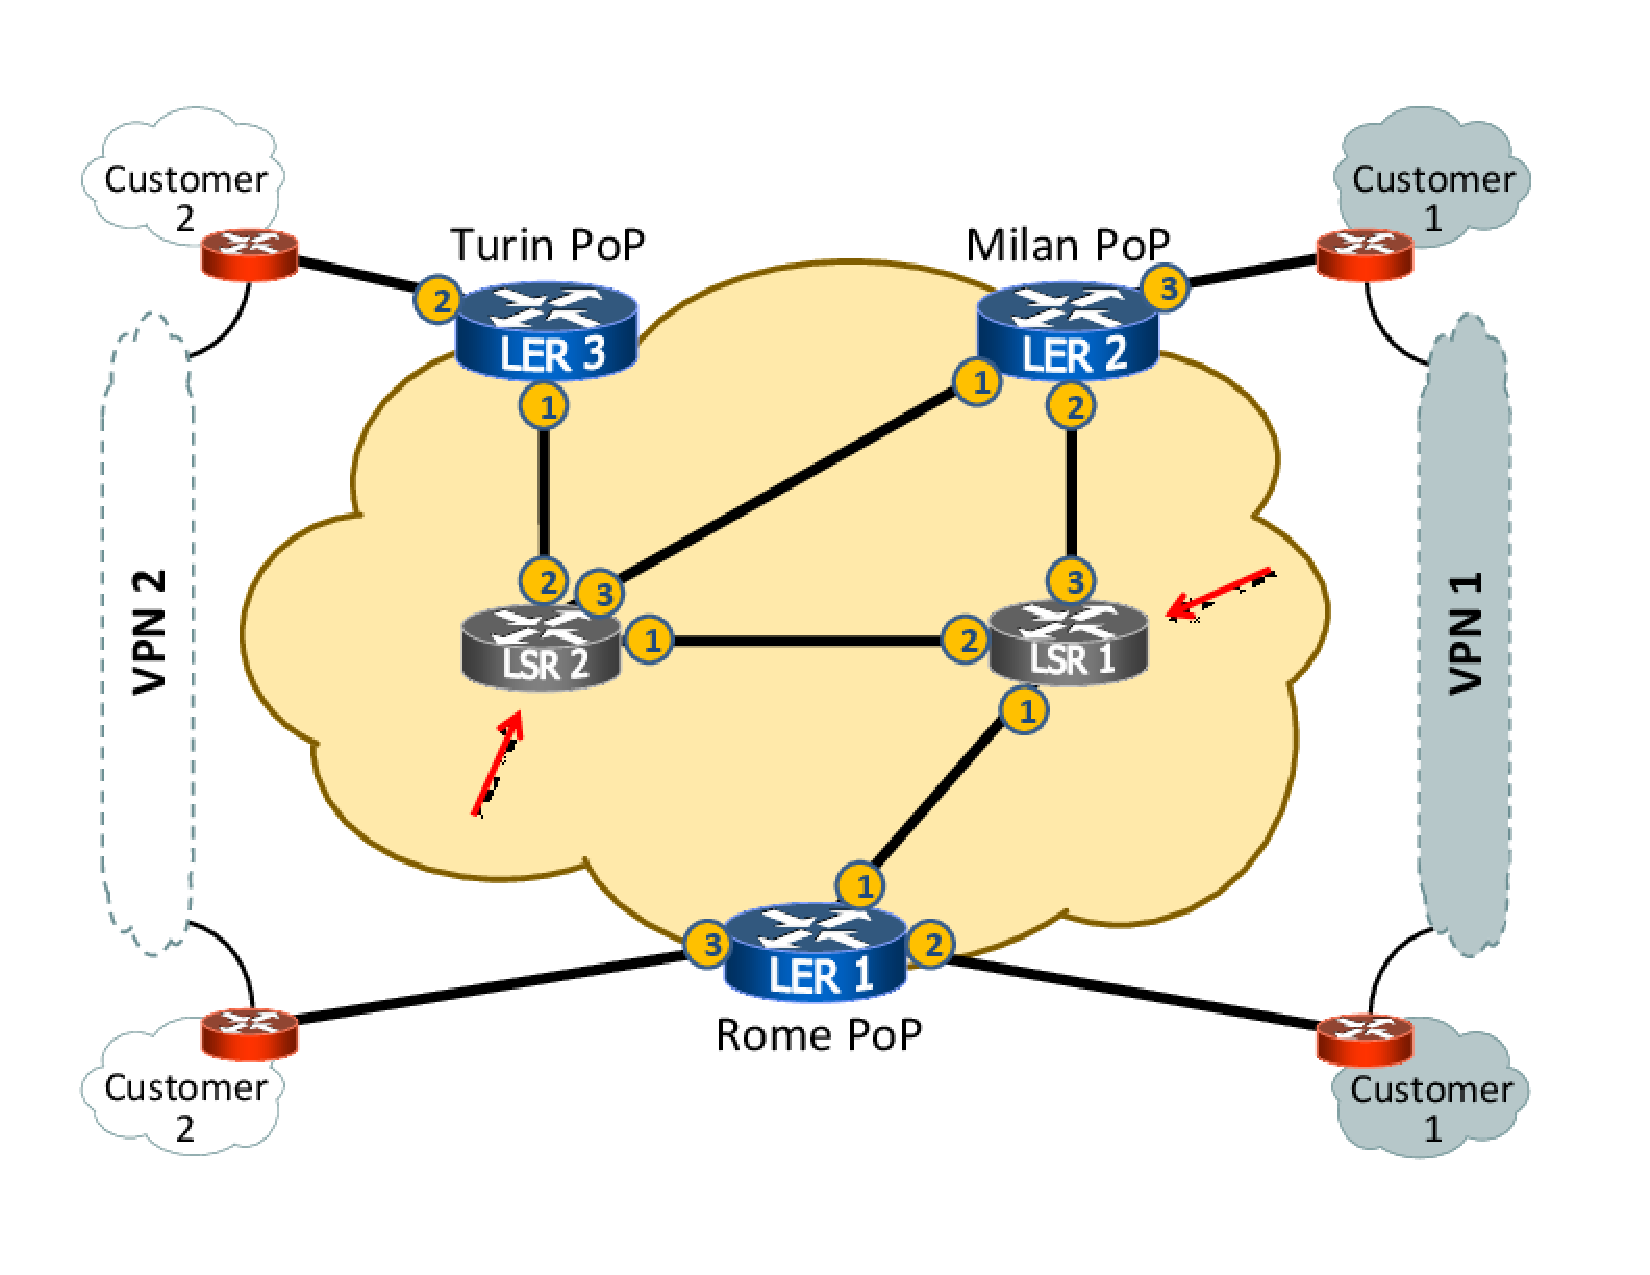
\includegraphics[width=0.7\columnwidth]{figures/mpls-slides-4}
%  \caption{P -- Provider Routers.}
%  \label{fig:mpls-slides-4}
% \end{figure}


\begin{shaded}
\noindent
Fig.~\ref{fig:mpls-slides-1} shows some details of the provider's infrastructure of our
scenario. It is
both an MPLS network and an IP network (it has an MPLS data plane and an IP data
plane).

If we look at it from the MPLS point of view, we can distinguish CE, PE, and P 
routers. The small, red routers placed at the customer premise in the corners 
of Fig.~\ref{fig:mpls-slides-1} are CE routers. CE routers are directly 
attached to the blue routers at the edge of the provider premise, which are the 
PE routers (or LERs). Finally, the grey routers in the core of the provider 
network are the P routers (or LSRs).
% The red arrows in Figs.~\ref{fig:mpls-slides-2}, \ref{fig:mpls-slides-3},
% and~\ref{fig:mpls-slides-4} show the CE routers, the PE routers, and the P-routers of
% our
% example network, respectively. Also, routers are labeled, according to the MPLS
% terminology, as LERs or LSRs.

Since the provider network is also an IP network an IP address is given to the interfaces.
To do this, our provider exploits prefix $80.0.0.0/8$. This prefix will not be announced
outside the provider's network. The reason for the presence of label AS100
in the provider network will be explained soon.

The two CE routers serving Customer $1$ are connected through a VPN called VPN1 
(on the right side of Fig.~\ref{fig:mpls-slides-1}). The two CE routers serving 
Customer $2$ are connected through a VPN called VPN2 (on the left side). 
\end{shaded}

%%%%%%%%%
%%%%%%%%%
%%%%%%%%%
%%%%%%%%%
\section{Checkmate VPNs in Three Moves}\label{se:overview}

In this section we give a high-level description of an MPLS VPN. Such a description is
based on three main ingredients that we call ``moves''. We claim that a reader that
understands these three moves will be able to checkmate this complex matter.

From the perspective of the customer, an MPLS VPN 
%is nothing more than a cloud which is transparent to IP packets: as if the customer's CE routers were 
%connected by a \emph{pseudowire} which traverses the cloud. 
simply routes IP packets among customers CE routers, as if they were connected by a \emph{pseudowire}.
Observe that, as customers may have overlapping address spaces, their packets cannot be simply routed through the provider network. Instead, they need to be encapsulated.  
It is tempting to implement such a pseudowire using a tunnel (e.g., GRE, IP-in-IP or IPSec) 
between PE routers where the customer packets travel across the provider network 
\emph{encapsulated} into IP or IPSec packets. However, as the number of 
interconnected sites grows, manually managing configured tunnels and maintaining 
forwarding tables becomes excessively complex. For example, if we were to use 
tunnels to implement an L3VPN over 5 customer sites, a full-mesh topology would 
translate to 20 manually configured tunnels. Moreover, if the customer adds a 
new subnet to one of its sites, we need to update the forwarding tables of all 
our 5 PE routers. Observe that the complexity
of managing tunnels can be eased by automatic setup mechanisms. However, such 
mechanisms are out of the scope of this chapter, therefore we refer the 
interested reader to~\cite{rfc4023,rfc5512,cisco-preso}.

The intrinsic problem with tunnels is that they rely on a pre-determined 
endpoint which is configured at tunnel setup time. Ideally, we would like to 
take advantage of the benefits of encapsulation without dealing with the 
issue of knowing the tunnel endpoint in advance. Namely, we would like packets 
to be encapsulated at the ingress PE and decapsulated at egress PE. We can 
split this goal into three high-level steps that we call moves:

\begin{enumerate}
\item[Move 1:] Achieve any-to-any IP connectivity among PEs,
\item[Move 2:] Define a signalling mechanism to distribute customer prefixes among PEs, 
and
\item[Move 3:] Define an encapsulation mechanism to transport packets from one 
PE 
to another across the network.
\end{enumerate}

One of the key benefits of using encapsulation (Move 3) is that the complexity 
of configuring L3VPNs for customers is confined to PEs. The core of the network 
(i.e., P routers) does not need to know anything about customer prefixes: it 
simply needs to know how to transport packets from one PE to another (Move 1). 
This means that the size of the forwarding table of P routers depends on the 
number of PE routers rather than on the number of customer prefixes. Finally, if PE 
routers use a signalling mechanism to dynamically synchronize the list of 
customer prefixes, the only pieces of information that need to be manually 
configured at each PE are the L3VPN identifier and the IP address of the CE 
router.

In the following we elaborate each move in more detail.

\subsection{Move 1 -- Any-to-any IP connectivity among PEs}
The first move is actually quite simple. It is nothing more than what any 
Internal Gateway Protocol (IGP) is designed to achieve: seamless, redundant and 
dynamic IP-level any-to-any connectivity. Since PEs are our encapsulation 
endpoints, we want them to be reachable independent of the availability of 
specific network interfaces. In other words, we do not want to use the IP 
address of physical interfaces for PEs, but loopback addresses. A loopback address is an address associated with a virtual 
interface of the router. Since it is virtual, a loopback interface it is active 
independent of the status of physical network interfaces. To fulfill Move 1, we 
simply assign a loopback address to each PE router and use an IGP (e.g. OSPF or 
IS-IS) 
%to ensure any-to-any connectivity among loopback addresses.
to announce these addresses as /32 prefixes in order to ensure any-to-any connectivity among them. 

\begin{figure}
\centering
 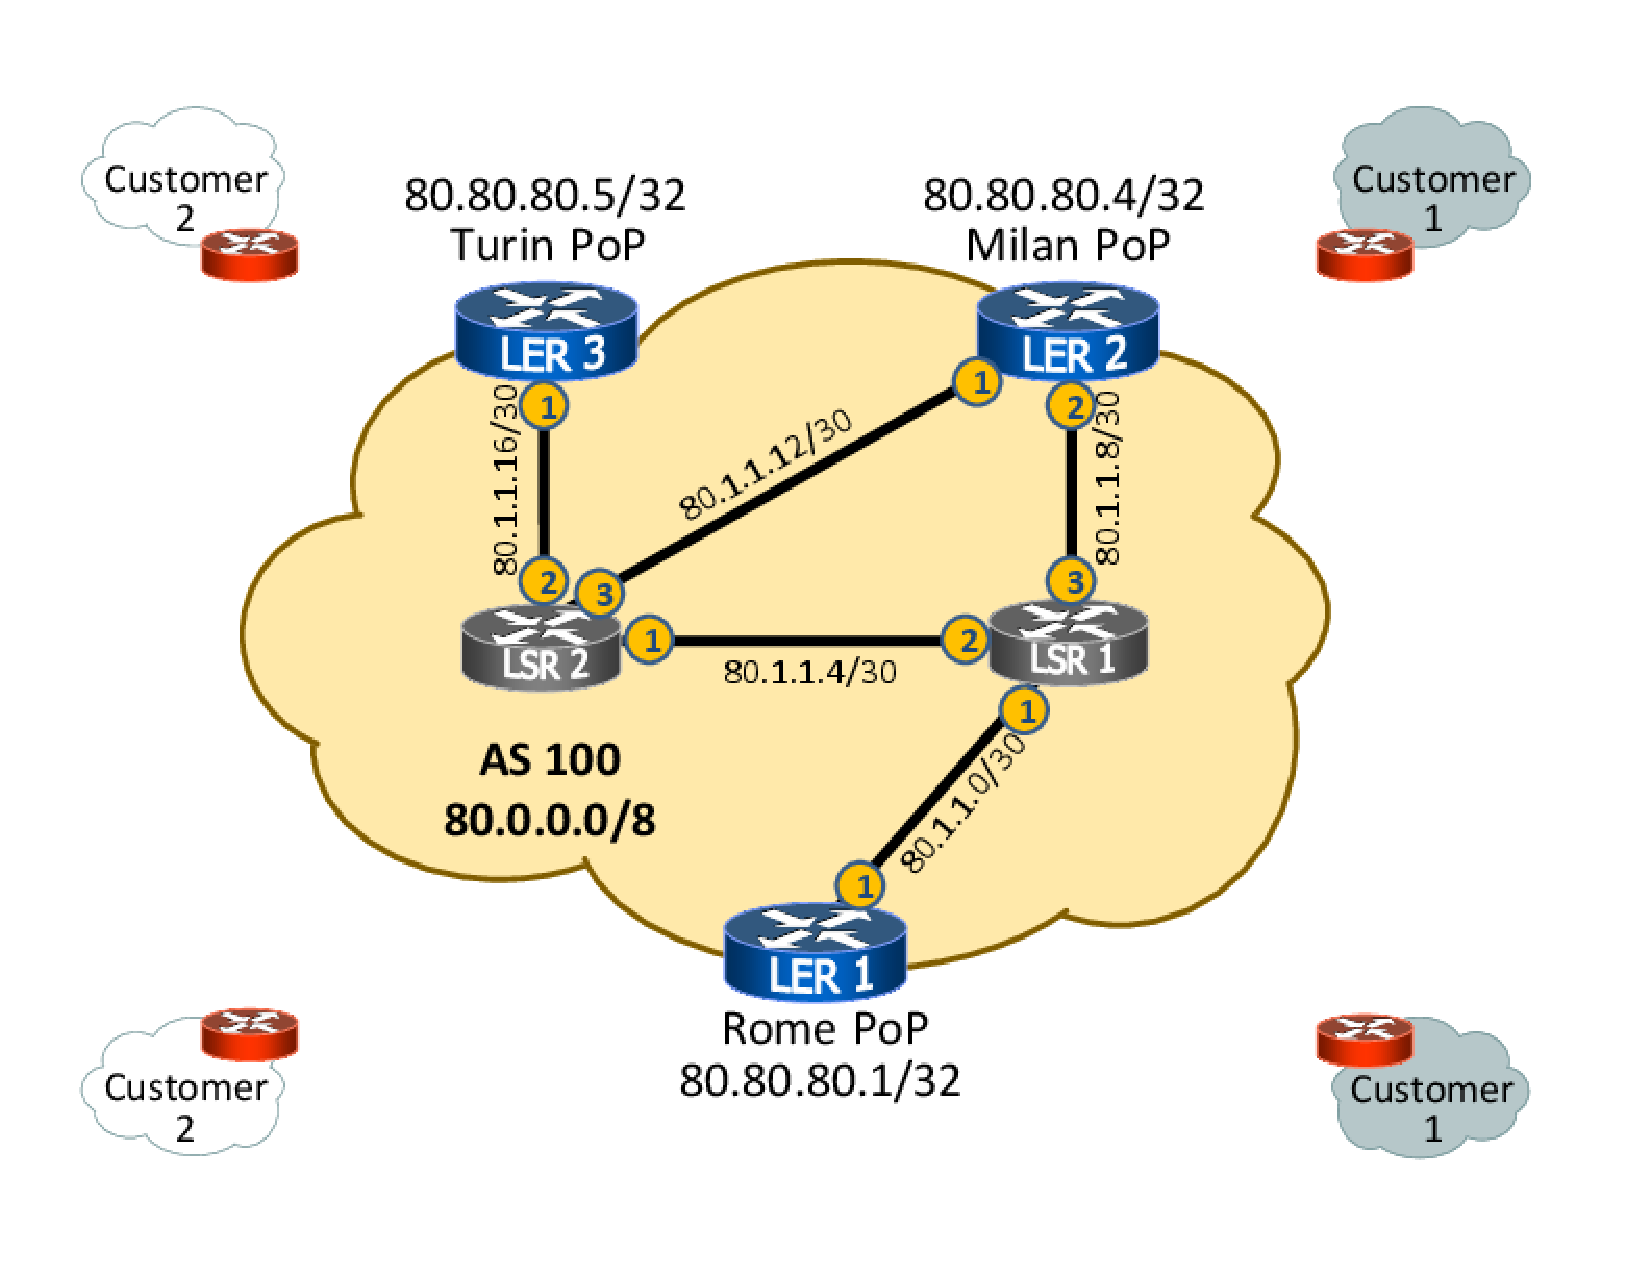
\includegraphics[trim=0cm 1.5cm 0cm 1.5cm, clip=true, width=0.7\columnwidth]{figures/mpls-slides-5}
 \caption{Loopbacks of PEs.}
 \label{fig:mpls-slides-5}
\end{figure}

\begin{figure}
\centering
 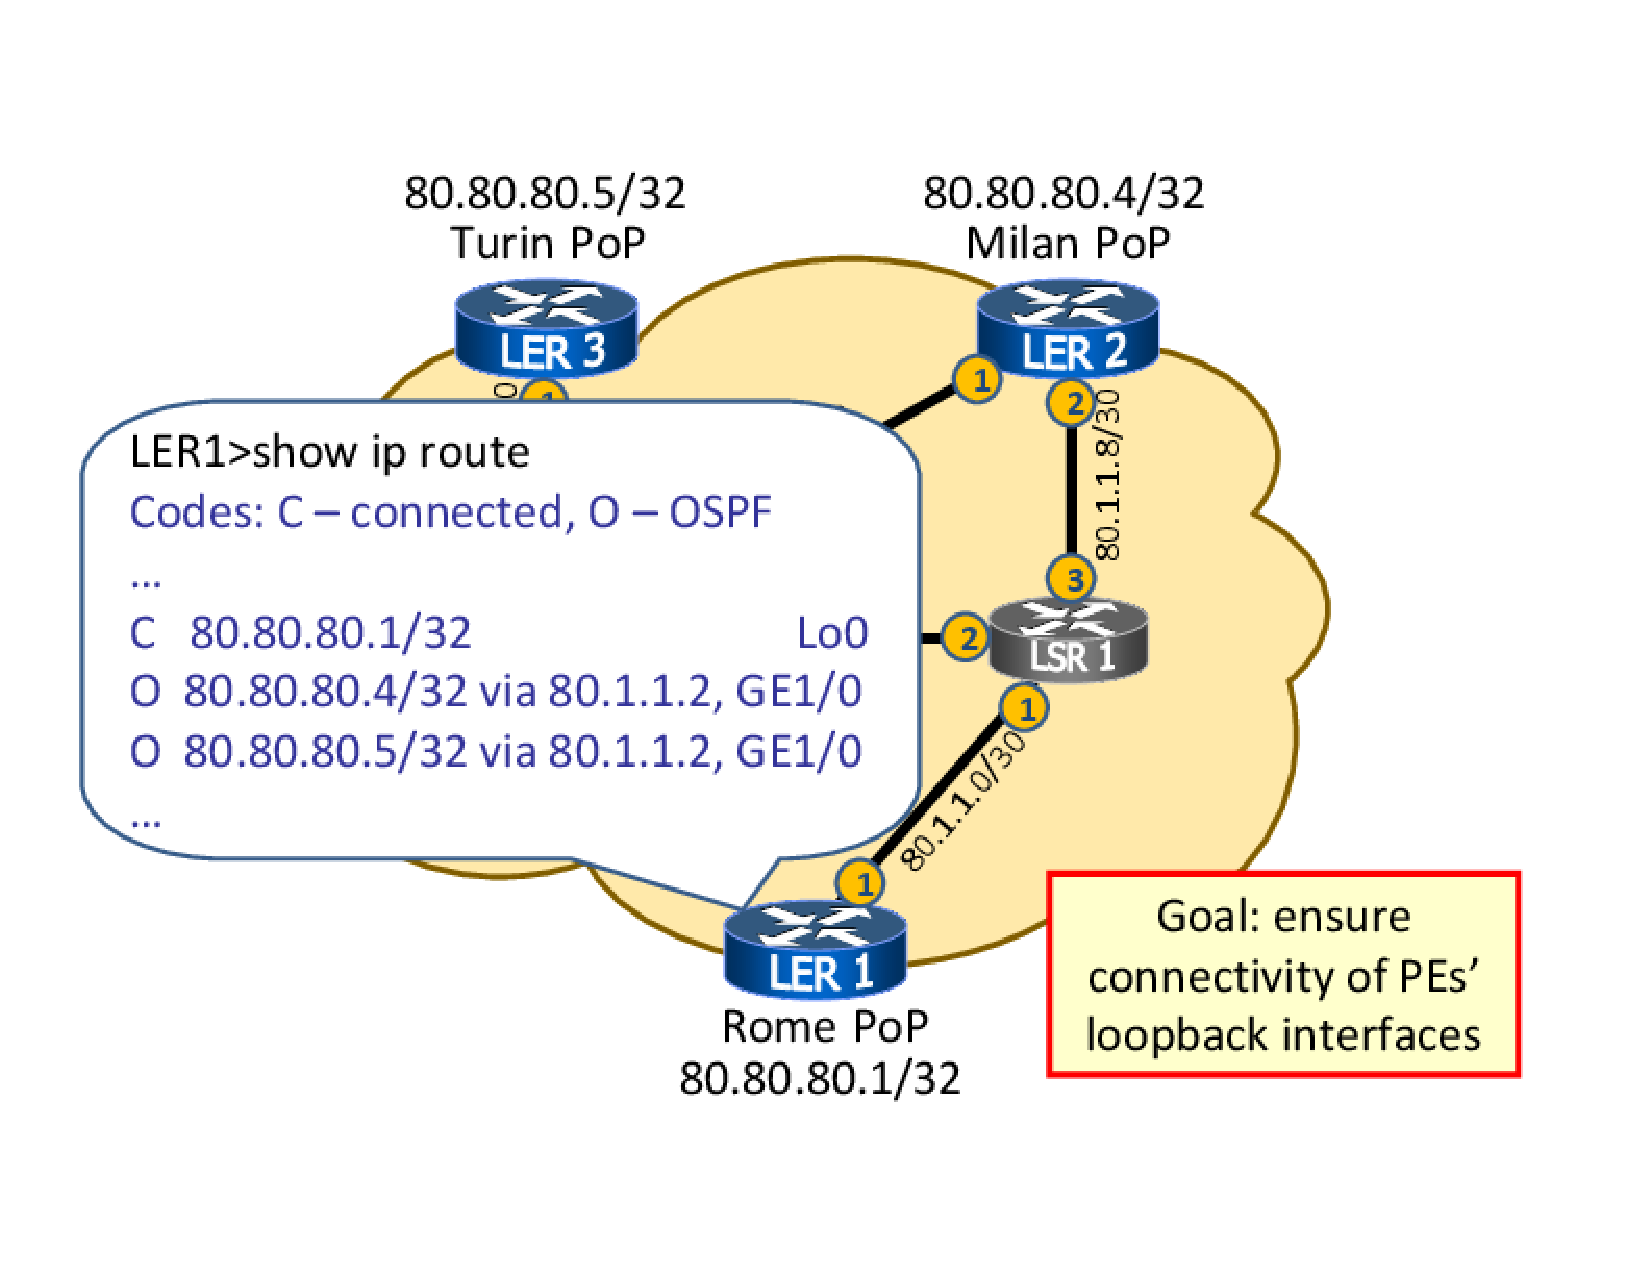
\includegraphics[trim=0cm 1.5cm 0cm 1.5cm, clip=true, width=0.7\columnwidth]{figures/mpls-slides-8}
 \caption{IP connectivity for LER1.}
 \label{fig:mpls-slides-8}
\end{figure}

\begin{figure}
\centering
 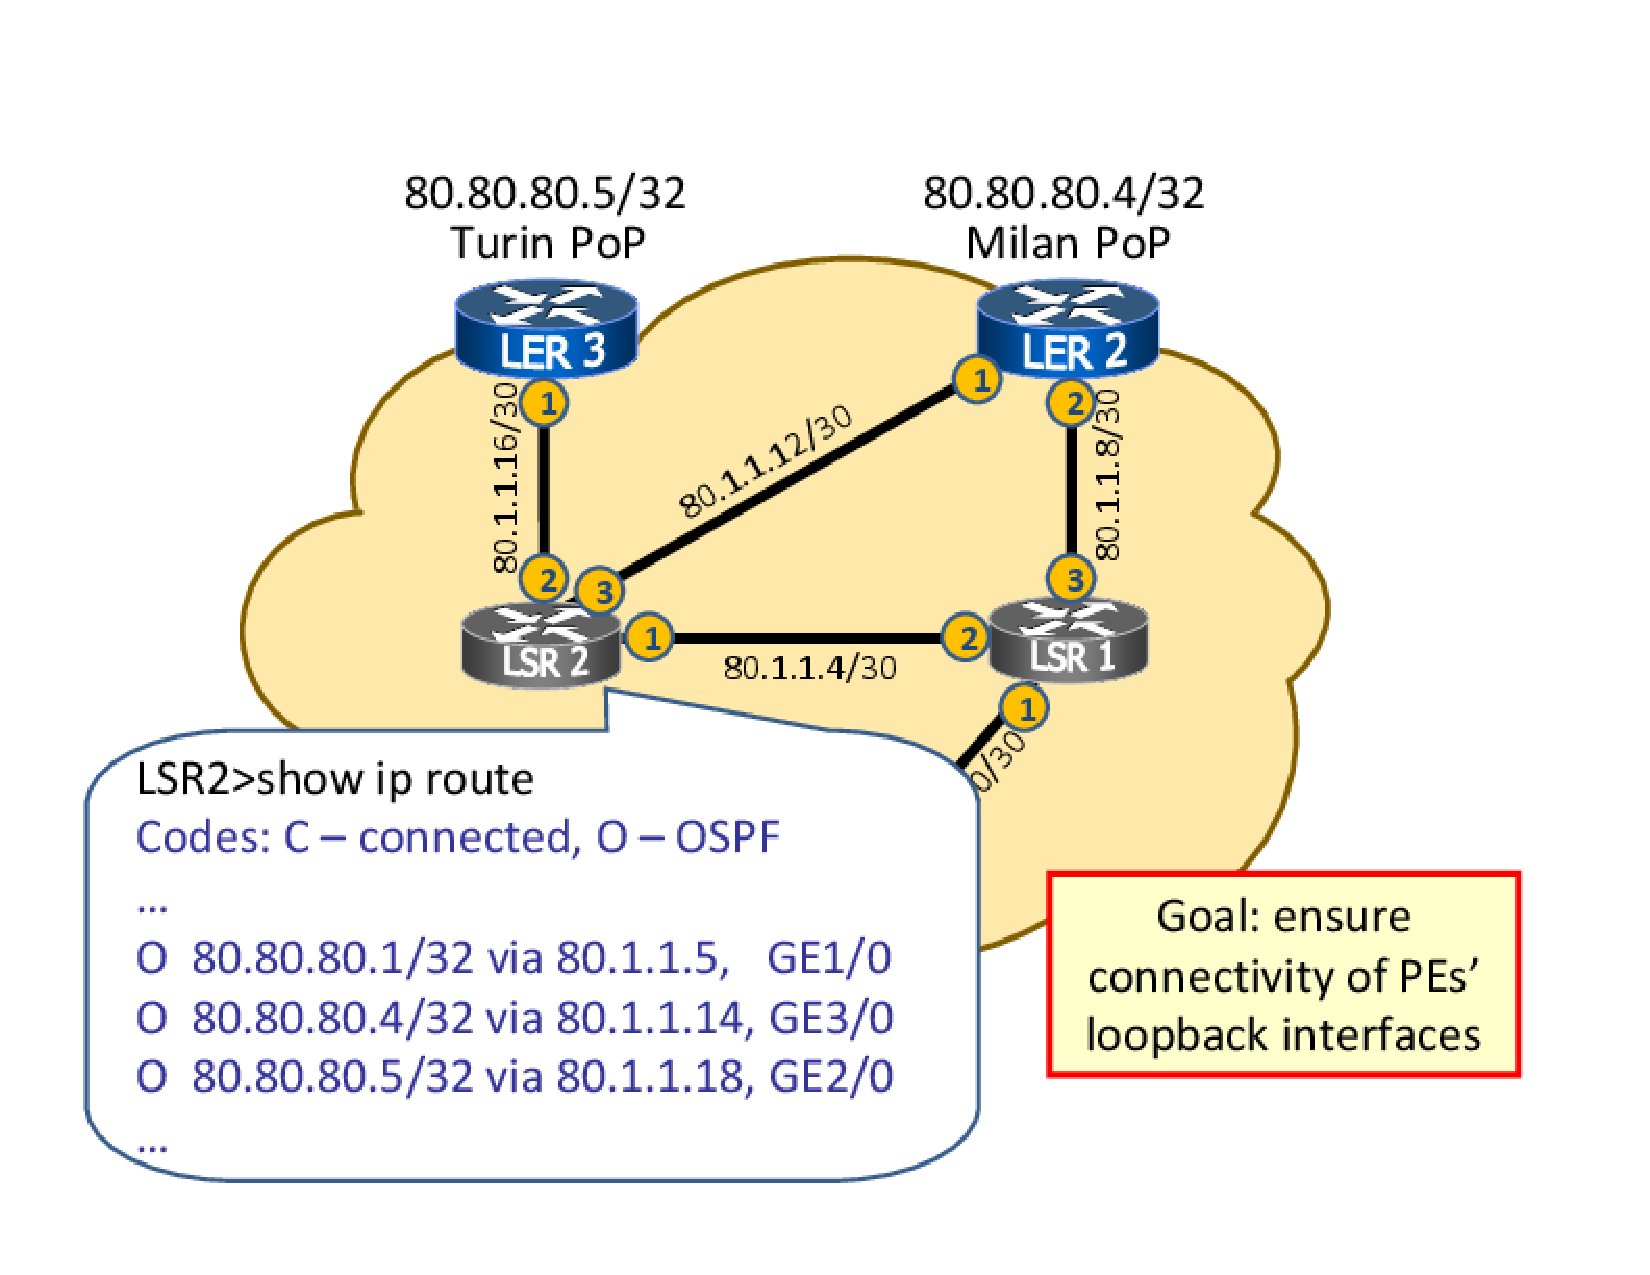
\includegraphics[trim=0cm 1.5cm 0cm 1.5cm, clip=true, width=0.7\columnwidth]{figures/mpls-slides-9}
 \caption{IP connectivity for LSR2.}
 \label{fig:mpls-slides-9}
\end{figure}

\begin{figure}
\centering
 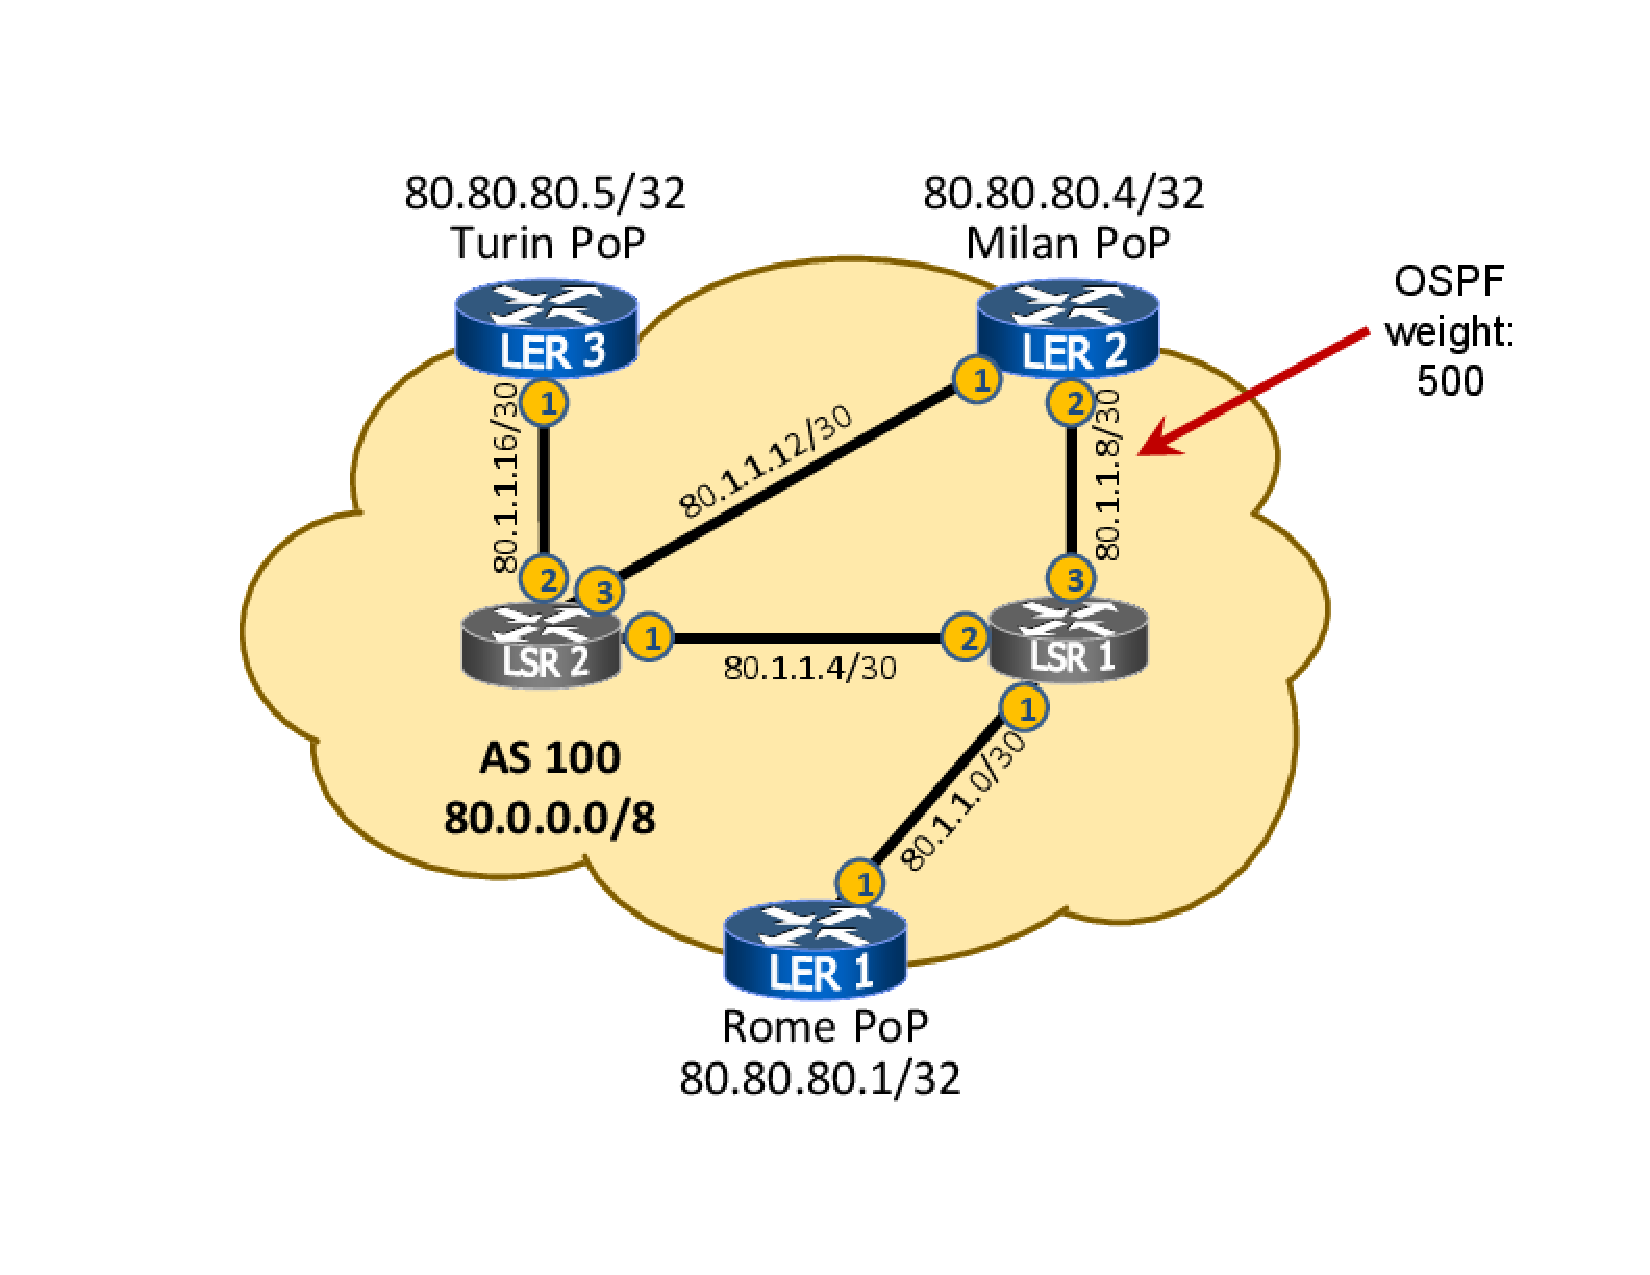
\includegraphics[trim=0cm 1.5cm 0cm 1.5cm, clip=true, width=0.7\columnwidth]{figures/mpls-slides-10}
 \caption{The OSPF weight of a link.}
 \label{fig:mpls-slides-10}
\end{figure}

\begin{shaded}
\noindent
Fig.~\ref{fig:mpls-slides-5}
shows the loopback addresses assigned to the PEs of our example network. Also, we assume
that routers use OSPF to propagate reachability information of loopbacks of
routers.

Configuring routers to fulfill Move 1 is straightforward. In our sample network, 
the configuration of LER1 for Move 1 is as follows.
% (throughout the chapter we show
% configuration snippets in a Cisco-like language; other vendors' languages accept very
% similar constructs).

\begin{codice}
\begin{verbatim}
  interface Loopback0
    ip address 80.80.80.1 255.255.255.255
  interface GigabitEthernet1/0
    ip address 80.1.1.1 255.255.255.252
  router ospf 10
    network 80.0.0.0 0.255.255.255 area 0
\end{verbatim}
\end{codice}

The first two lines assign an IP address to interface \texttt{loopback0}. The second pair
of lines assign an IP address to interface \texttt{GigabitEthernet1/0} that connects LER1
with LSR1. The last two lines activate OSPF protocol.

Fig.~\ref{fig:mpls-slides-8} shows the result of command {\tt show ip route} performed on
router LER1. Fig.~\ref{fig:mpls-slides-9} shows the result of command {\tt show ip route} 
performed on router LSR2. Command {\tt show ip route} has the effect of showing the
control plane routing table of routers.

In order to force a more interesting routing in
the following part of the example, we set OSPF weight $500$ for a specific link,
discouraging the use of that link by the IGP routing
protocol, as shown in Fig.~\ref{fig:mpls-slides-10}. 
\end{shaded}

\subsection{Move 2 -- Use BGP to distribute customer prefixes}
In order to distribute reachability information about customer prefixes, MPLS 
relies on a variant of BGP called Multi-Protocol BGP (MP-BGP)\cite{rfc2858}. 
Whereas BGP advertises reachability information for IPv4 addresses only, MP-BGP 
supports multiple \emph{address families} (e.g., IPv4 and IPv6). Since 
advertising VPN addresses implies exchanging not only IPv4 prefixes, but also 
additional information to identify the VPN, MP-BGP treats VPNs as a separate 
address family. PE routers establish a full-mesh of iBGP peerings and each PE 
announces to all the other PEs the customer prefixes that it can reach via the 
CE router it is connected to. The Multi-Protocol extension to BGP is needed to 
introduce the concept of the ``customer'' (i.e., the ``L3VPN identifier'') which 
does not exist in plain BGP. 

Compared with any ad-hoc signalling mechanism that could have been designed 
specifically for MPLS, the choice of using BGP has the advantage of relying on a 
well-known protocol and thus making the learning curve smoother for 
practitioners. Moreover, BGP has built-in mechanisms (e.g., route reflection) to 
scale as the number of PE routers increases.

\begin{figure}
\centering
 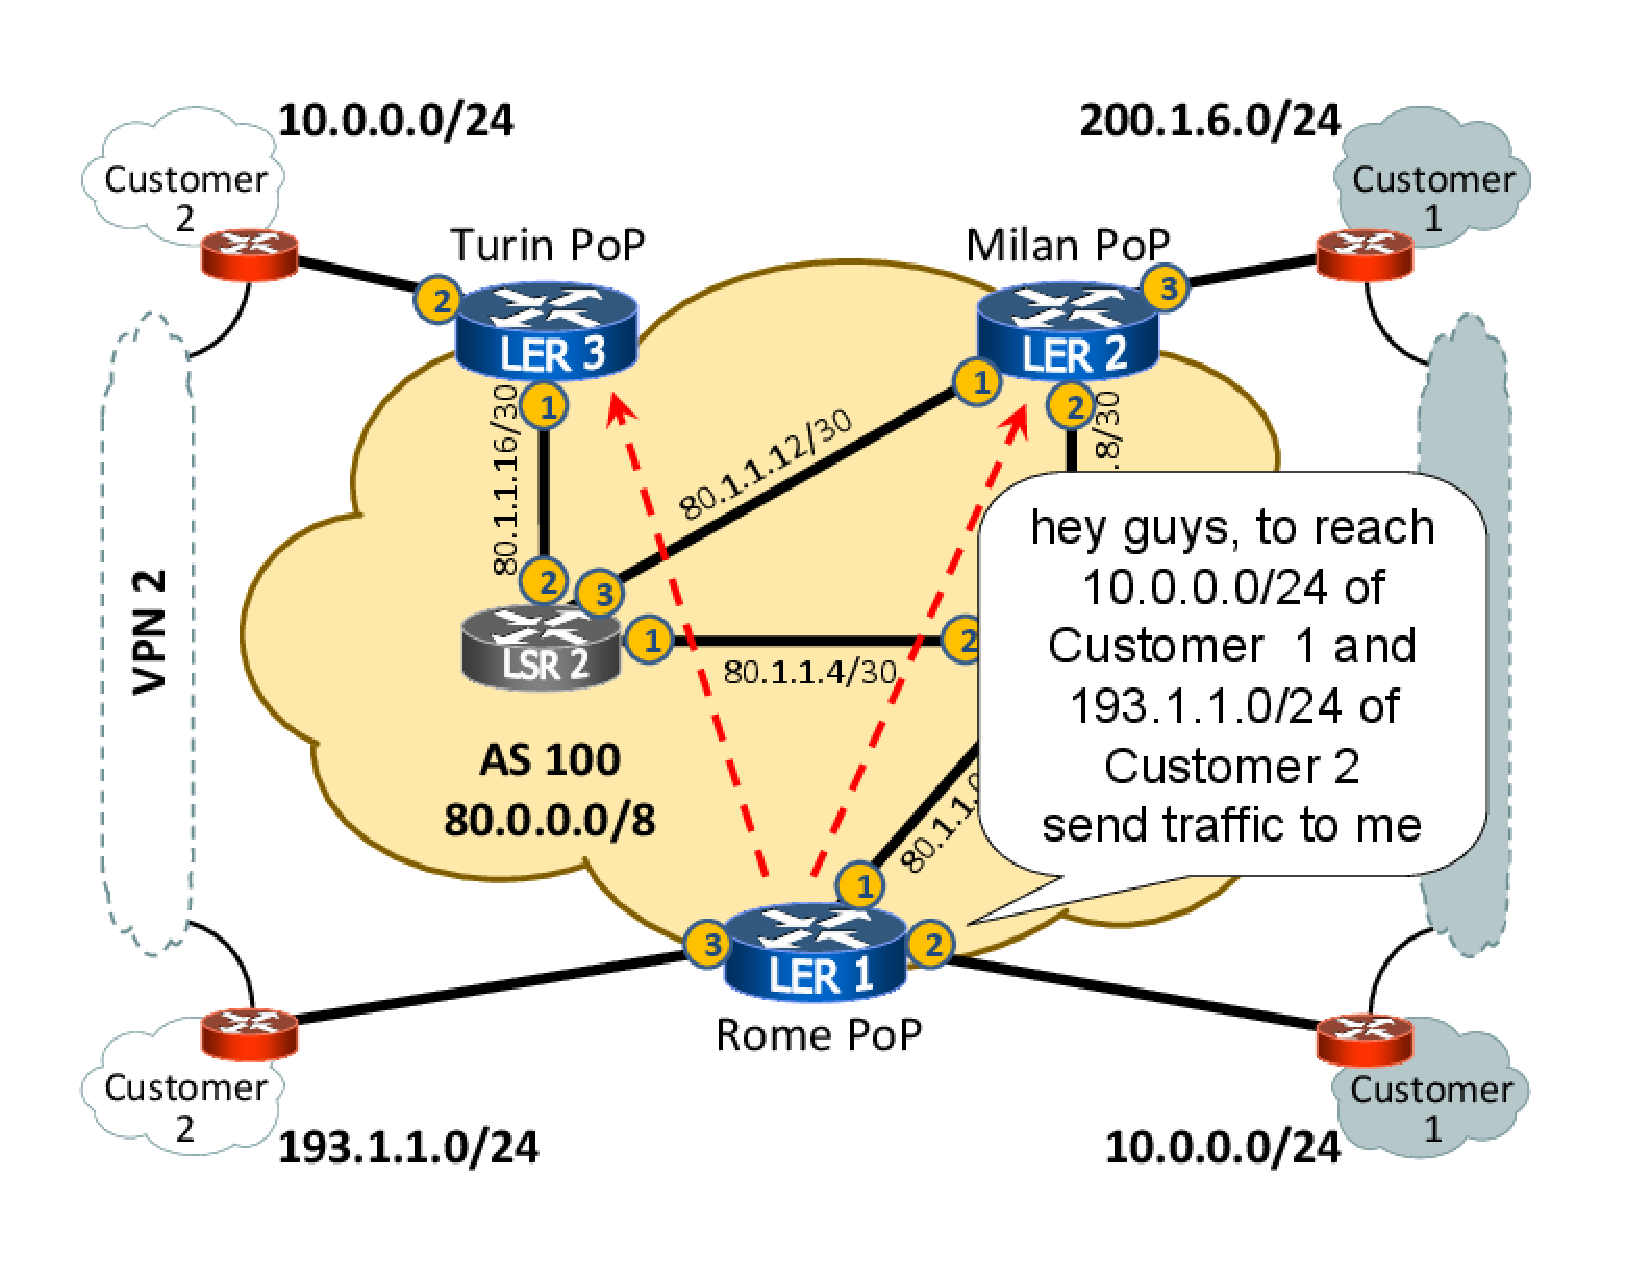
\includegraphics[trim=0cm 1.5cm 0cm 1.5cm, clip=true, width=0.7\columnwidth]{figures/mpls-slides-6}
 \caption{Use of BGP to distribute customer prefixes.}
 \label{fig:mpls-slides-6}
\end{figure}

\begin{shaded}
\noindent
Fig.~\ref{fig:mpls-slides-6} shows a high-level illustration 
of how the BGP peerings with LER3 and LER2 can be used by LER1 to announce 
customer prefixes.
\end{shaded}

\vspace{0.1cm}

\begin{shaded}
\noindent
Configuring MP-BGP peerings is very similar to configuring plain iBGP
peerings. 
Consider the following snippet from the configuration of router LER1:
\begin{codice}
\begin{verbatim}
  router bgp 100
    neighbor 80.80.80.4 remote-as 100
    neighbor 80.80.80.4 update-source Loopback0
    neighbor 80.80.80.5 remote-as 100
    neighbor 80.80.80.5 update-source Loopback0
    !
    address-family vpnv4
      neighbor 80.80.80.4 activate
      neighbor 80.80.80.5 activate
    exit-address-family
\end{verbatim}
\end{codice}

The first line starts the BGP configuration and states that the router belongs to AS100.
Observe that all the routers are supposed to belong to Autonomous System (AS) 100. This
AS number will not be necessarily propagated outside the provider's network and is only
needed to establish peerings between PEs.

The following lines specify the BGP peerings. The presence of the ``\texttt{vpnv4}''
address family identifies LER2 and LER3 as MP-BGP neighbors of LER1.
\end{shaded}

\subsection{Move 3 -- Use MPLS encapsulation among PEs}
Having performed Move 1 and Move 2, a PE router $r$ is able to select the PE 
router $r'$ that is connected to a given customer prefix (by Move 2). Also, $r$ is 
able to forward IP packets to $r'$ (by Move 1). The only piece missing is an 
encapsulation mechanism to transport IP packets from $r$ to $r'$. One such 
encapsulation mechanism is MPLS: the PE router $r$ encapsulates the IP packet by 
pushing two MPLS labels. The label at the top of the stack (\emph{outer} label) 
is switched by P routers in order to deliver the packet to router $r'$. The 
label at the bottom of the stack (\emph{inner} label) is left untouched and it 
is used by the egress PE $r'$ to identify the correct L3VPN. Observe that the 
inner label is necessary because $r$ and $r'$ could serve a variety of 
customers, and address spaces might be overlapping. For instance, routers $r$ 
and $r'$ could be serving two distinct VPNs for two customers, both using 
addresses in the RFC 1918 space.

Let us briefly recap how a packet is delivered across an MPLS cloud. When PE 
router $r$ receives a packet from a CE router, it picks the VPN identifier and 
the destination address and, based on information contained in its MP-BGP 
Routing Information Base (RIB), it finds the PE router the packet should be 
delivered to. The MP-BGP RIB also contains the inner label that should be used. 
In our running example, the egress PE router is $r'$. Then, $r$ pushes the inner 
MPLS label and an outer label which is guaranteed to deliver the packet to 
$r'$. 

How does $r$ pick this outer label? The outer label that maps to router $r'$ is 
determined by the Label Forwarding Information Base (LFIB) of $r$, which is the 
forwarding table for MPLS.

The task of distributing labels and maintaining the LFIB of label switch routers 
is performed by the Label Distribution Protocol 
(LDP)\cite{rfc5036}\footnote{Alternative protocols such as RSVP and BGP can also 
serve the same purpose, but are out of the scope of this chapter.}. LDP is able 
to setup a Label Switch Path (LSP) from one PE to another. In its simplest form, 
LDP maps an address prefix FEC (i.e., a FEC which represents an IP prefix) to a 
label. Each router receives LDP mappings from all its neighbors. In order to 
populate the LFIB, each router inspects its own forwarding table to determine 
the IP nexthop for the FEC, and picks the corresponding label. This way, LDP 
effectively creates a forwarding tree rooted at the egress point of the FEC, by 
simply importing the nexthop from the IP data plane (remember Move 1) at each 
intermediate hop.

\begin{shaded}
\noindent
It is extremely simple to configure a router to fulfill Move 3, because the LDP 
protocol can be safely run in the default configuration, and enabling MPLS 
encapsulation on specific interfaces is a single command. The configuration of 
LER1 for Move 3 is as simple as the following.

\begin{codice}
\begin{verbatim}
mpls label protocol ldp
interface GigabitEthernet1/0
  ip address 80.1.1.1 255.255.255.252
  mpls ip
\end{verbatim}
\end{codice}
\end{shaded}
%%%%%%%%%
%%%%%%%%%
%%%%%%%%%
%%%%%%%%%
%%%%%%%%%
\section{An In-Depth View of MPLS VPNs}\label{se:details}

We have seen that the architecture of MPLS VPNs builds upon three building 
blocks: a working IP data plane that is capable of interconnecting the loopback 
addresses of PE routers, a BGP-based control plane to distribute reachability 
information about customer prefixes, and MPLS encapsulation among PEs.

While the first building blocks might seem straightforward at a first glance, 
there are a number of details which complicate the big picture but 
nevertheless are important in order to grasp the internals of MPLS 
VPNs.

%
%%%
%%%%%
%%%
%
\subsection{IP Data Plane}
IP connectivity between PE routers is easy to achieve using any suitable routing 
protocol. However,
PE routers might be attached to a number of CEs of different 
customers, and must ensure that each CE is mapped to the correct VPN. A 
traditional IP data plane is unfit for this purpose since the IP address space 
of customers can overlap. Hence, a PE router must be able to route packets based 
on both the IP address and the specific VPN the packet belongs to. To accomplish 
this task, MPLS VPNs exploit a technique called Virtual Routing and Forwarding 
(VRF) which allows a router to have multiple (virtual) routing tables, 
potentially a separate virtual routing table for each network interface (either 
physical or logical). With this technique, mapping a CE to the correct VPN is as 
easy as configuring the corresponding interface within a specific VRF table. 
An MPLS inner label actually identifies a VRF instance.

One way to implement VRF while still maintaining a single forwarding table is 
using the ingress interface as an additional input parameter in the forwarding 
table. In such an implementation, the organization of the forwarding table of a 
router would be the one illustrated in Table~\ref{tab:fib-destination-vrf}. 
Observe that only the PE router needs to support VRF. The CE router is 
configured with a plain eBGP configuration and is completely unaware of the VRF 
implemented on the provider side.

\begin{table}
 \centering
 \begin{tabular}{|c|c|c|c|}
 \hline
 \textbf{VRF id} & \textbf{Ingress interface} & \textbf{Destination address} & 
\textbf{Egress interface} \\
 \hline
 VRF-3 & en5 & 10.100.200.32 & en2 \\
 \hline
 \end{tabular}
 \caption{Structure of the forwarding table in the ``forwarding by network 
address'' approach with Virtual Routing and Forwarding (VRF).}
 \label{tab:fib-destination-vrf}
\end{table}

\begin{shaded}
\noindent
Assigning an interface to a specific VRF instance is straightforward. In our 
sample network, we configure router LER1 as follows.\\

\begin{codice}
\begin{verbatim}
  interface GigabitEthernet2/0
    ip vrf forwarding VPN1
    ip address 10.0.0.1 255.255.255.0
  interface GigabitEthernet3/0
    ip vrf forwarding VPN2
    ip address 193.1.1.1 255.255.255.0
\end{verbatim}
\end{codice}

Address \texttt{10.0.0.1} is the address assigned to the interface that connects LER1
to Customer 1, while address \texttt{193.1.1.1} is assigned to the interface that
connects LER1 to Customer 2.
\end{shaded}



%
%%%
%%%%%
%%%
%
\subsection{MP-BGP Control Plane}
Multi-protocol extensions to BGP allow us to segregate each L3VPN in a different 
\emph{namespace}, identified by a proper VPN identifier. Separating namespaces 
is important because an IP prefix is not guaranteed to be unique across multiple 
VPNs: in practice, customers might want to use their own private IP address 
spaces, possibly overlapping with the address space of other customers. MP-BGP 
solves this issue by introducing the concept of VPN-IP addresses, that is, IP 
addresses tagged with a 8-byte VPN identifier which is called \emph{route 
distinguisher} (RD). A VPN-IP address is nothing more than the concatenation of 
the RD and the IP prefix. By imposing that different VPNs be assigned distinct 
RD values, the uniqueness of VPN-IP addresses is guaranteed even in the presence 
of overlapping IP address space among customers. A special RD value consisting 
of 8 NULL bytes represent the default VPN, which allows MP-BGP to distribute 
information regarding pure IP routes alongside information about VPN-IP prefixes.

Observe that, while a VPN-IP prefix uniquely identifies a destination, it 
provides no information about the reachability of that destination. For this 
reason, MP-BGP messages associate VPN-IP prefixes with the MPLS labels that 
should be used for forwarding.

\begin{figure}
\centering
 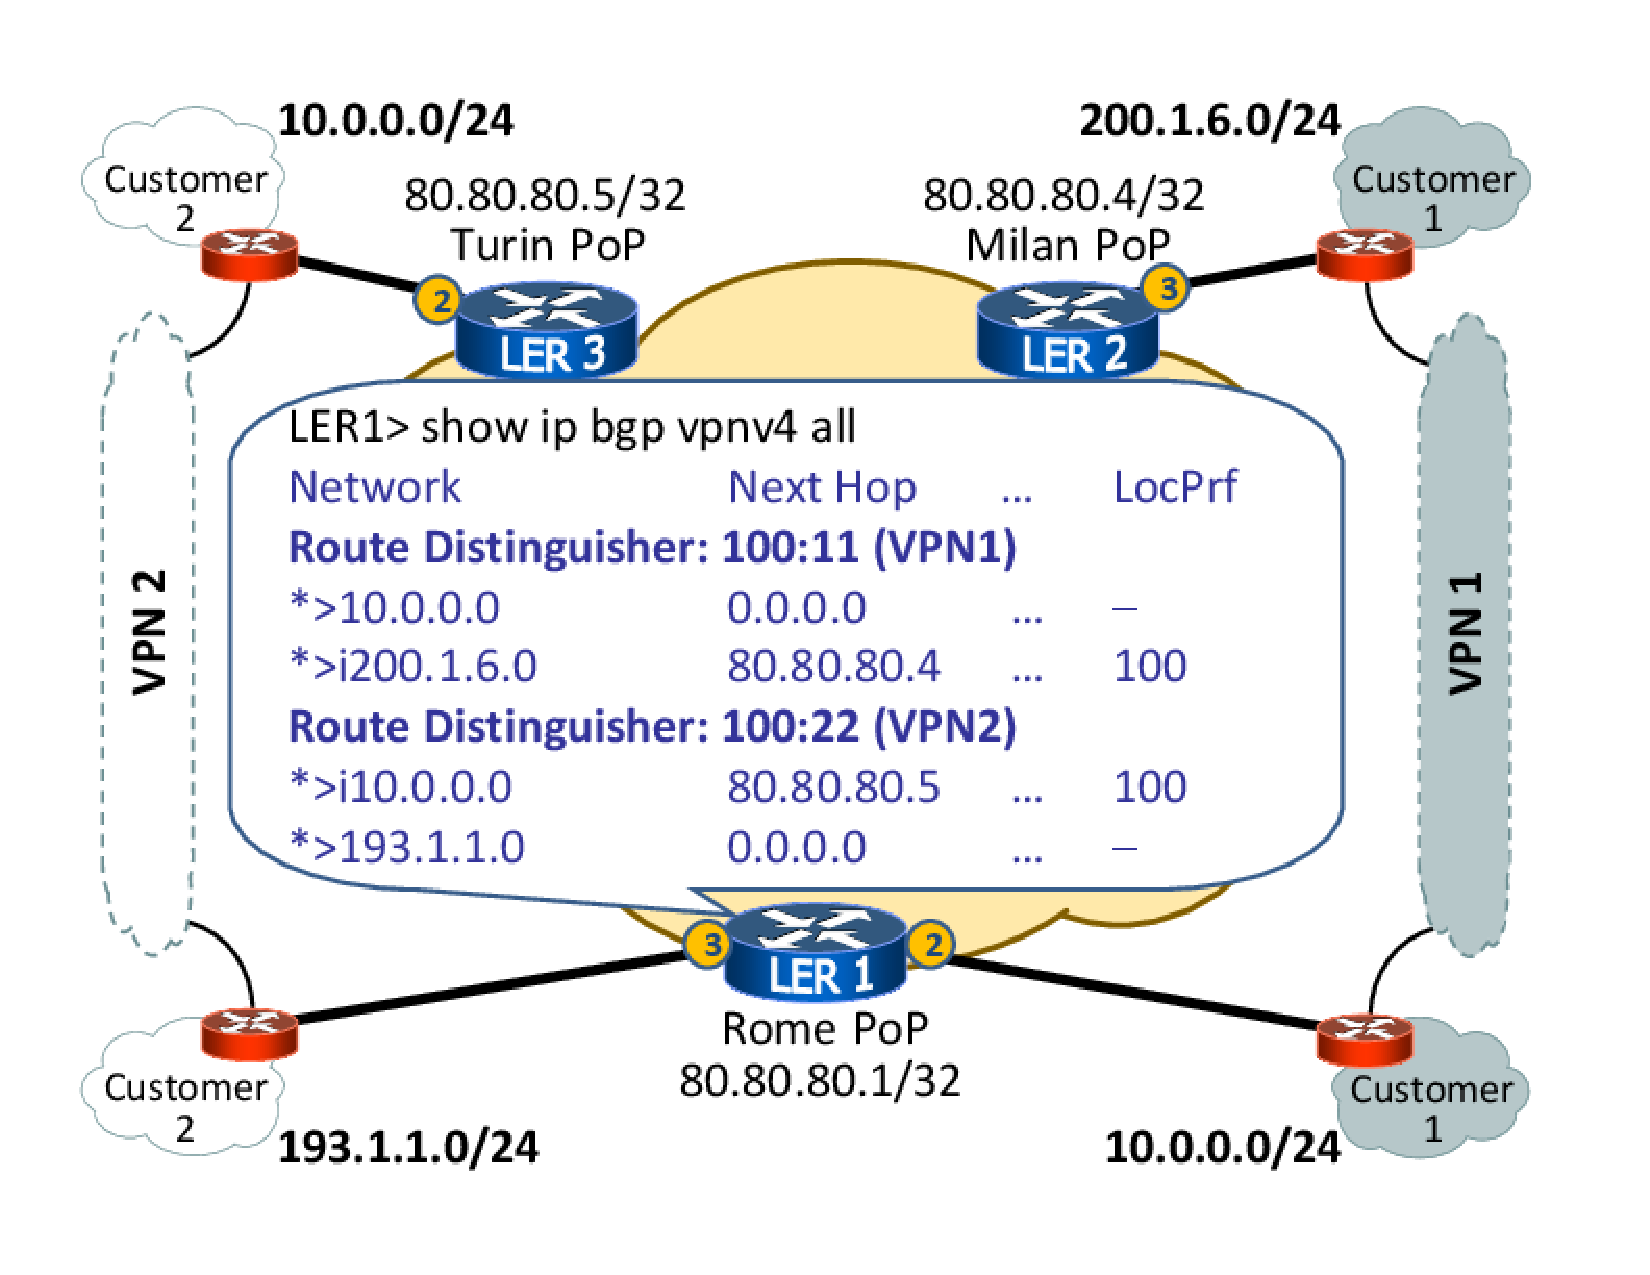
\includegraphics[trim=0cm 1.5cm 0cm 1.5cm, clip=true, width=0.7\columnwidth]{figures/mpls-slides-12}
 \caption{How MP-BGP can distribute per-VPN reachability information. Observe that the Local Preference attribute is not meaningful for locally originated prefixes, which are automatically preferred by the BGP decision process.}
 \label{fig:mpls-slides-12}
\end{figure}


\begin{shaded}
\noindent
It is easy to assign an RD value to a single VRF instance:\\

\begin{codice}
\begin{verbatim}
ip vrf VPN1
  rd 100:11
ip vrf VPN2
  rd 100:22
\end{verbatim}
\end{codice}

Fig.~\ref{fig:mpls-slides-12} shows the output of command {\tt show ip bgp vpnv4 
all} on router LER1. This command has the same effect of {\tt show ip bgp} but 
it shows the routing entries related to IPv4 VPNs. In this case the output highlights 
that LER1, in addition to its locally originated prefixes 10.0.0.0/24 with Route Distinguisher 100:1 and 193.1.1.0/24 with Route Distinguisher 100:2, knows two remote prefixes. Namely, it knows 200.1.6.0 with 
Route Distinguisher 100:11 and 193.1.1.0/24 with Route Distinguisher 100:22.
\end{shaded}

Tagging IP prefixes with a VPN identifier is an easy solution, but it is 
suboptimal in a specific use case which has seen increasing popularity 
recently: the so-called \emph{extranets}. In its simple definition, an extranet 
is simply a connection between two different VPNs that are guaranteed to have 
non-overlapping IP address spaces. A realistic example might be a specific 
site of one customer that needs to connect to another specific site of 
another customer. A naive implementation of extranets would define an ad-hoc 
VPN and assign it a new RD value. However, this solution is undesirable because 
it creates multiple VPNs that have duplicate entries, yielding a waste of 
router memory (to store the entries) and a waste of router's CPU time (to 
process update messages that are identical but for the RD value).

In order to overcome such limitations, MPLS decouples the concept of route 
distinguisher, which is used to segregate the address space in multiple 
namespaces, from the concept of \emph{route target} (RT) which is another tag 
that is used to control which routes are imported in a given VPN and, 
similarly, which routes are exported from a given VPN. The route target is 
transported by MP-BGP using extended communities. More precisely, by 
exporting a route from a VPN we attach a user-defined RT community to all 
VPN-IP prefixes belonging to that VPN. On the other hand, by importing a 
given RT into a VPN we accept that every route having that RT value will 
be visible from the devices in that VPN.

\begin{shaded}
\noindent
Each VRF instance can be configured to import or export routes labelled with a 
specific Route Target value. In our simple example, assuming that no extranet 
connectivity is required between Customer 1 and Customer 2, each VRF instance 
can simply import a single RT value, as the following configuration snippet of 
LER1 shows:

\begin{codice}
\begin{verbatim}
  ip vrf VPN1
    rd 100:11
    route-target export 100:1000
    route-target import 100:1000
  ip vrf VPN2
    rd 100:22
    route-target export 100:2000
    route-target import 100:2000
\end{verbatim}
\end{codice}

This means that all the prefixes of VPN1 announced via MP-BGP by LER1 to any other PE
are tagged with RT 100:1000. Also, any prefix that is tagged 100:1000 and is announced to
LER1 via MP-BGP is imported into the VRF of VPN1. The configuration for VPN2 is similar.
\end{shaded}

\begin{shaded}
\noindent
Route Targets provide network operators with the flexibility of leaking specific 
routes into specific VRF instances, easing the deployment of extranets. Route 
Targets are transported in MP-BGP messages as extended BGP communities. For 
this reason, the configuration of MP-BGP peers needs to specify that the peer 
supports extended communities (which are disabled by default).

\begin{codice}
\begin{verbatim}
  router bgp 100
    address-family vpnv4
      neighbor 80.80.80.4 activate
      neighbor 80.80.80.4 send-community both
      neighbor 80.80.80.5 activate
      neighbor 80.80.80.5 send-community both
    exit-address-family
\end{verbatim}
\end{codice}
\end{shaded}

\begin{shaded}
\noindent
To better understand the interplay between MP-BGP and the Route Targets, let us look 
at the content of an MP-BGP packet captured in our network (see
Fig.~\ref{fig:mpls-slides-26}). Observe how the route target in the blue frame is
contained in the extended communities. 

The announcements tells to the MP-BGP peer receiving it that the packets that will be
received with the inner MPLS label 24 (red frame in the picture) will refer to the
specified route target and the specified route distinguisher (green frame in the picture).
\end{shaded}


\begin{figure}
\centering
 \frame{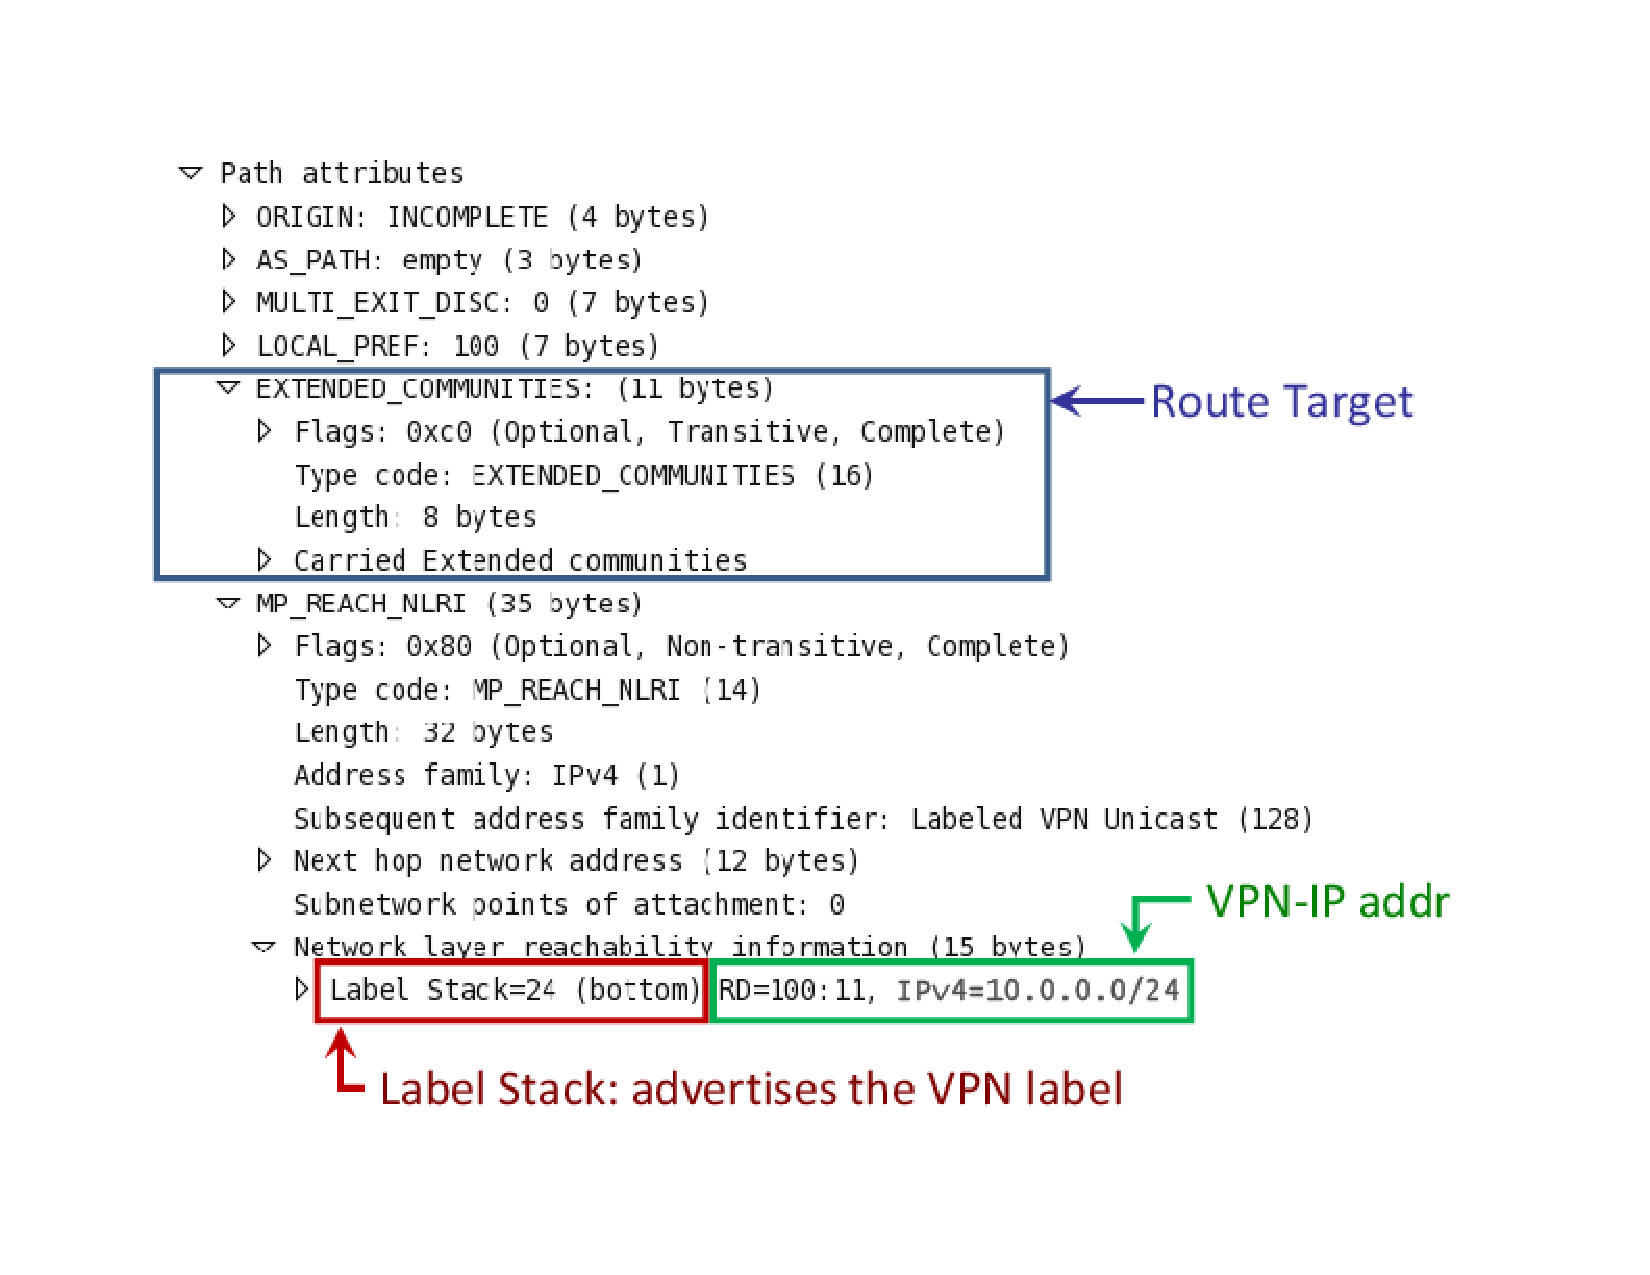
\includegraphics[trim=0cm 2.5cm 0cm 2.5cm, clip=true,
width=0.9\columnwidth]{figures/mpls-slides-26}}
 \caption{An MP-BGP signaling packet captured over the network.}
 \label{fig:mpls-slides-26}
\end{figure}


%
%%%
%%%%%
%%%
%
\subsection{MPLS Control and Data Plane}
The task of MPLS control plane is simply to establish Label Switched Paths 
(LSPs) between the loopback addresses of PE routers. LDP is in charge of 
populating and maintaining routers' LFIBs that implement the LSPs. In its most 
popular distribution mode, called \emph{unsolicited downstream}, LDP works in 
the following way. Each router creates a label for locally originated prefixes 
(e.g., the loopback address). The binding between a label and a locally 
originated prefix is called a \emph{local} binding. By contrast, a \emph{remote} 
binding is a binding between a label and a remotely originated prefix. Each 
router advertises its local bindings to its neighbors. When a neighboring router 
receives a binding for prefix $p_1$ and label $l_1$ on interface $i_1$, it looks 
up its IP forwarding table to check whether the advertised prefix is routed on 
interface $i_1$. If this is the case, it picks another label $l_2$ and starts 
announcing a binding for $p_1$ and $l_2$. Meanwhile, it updates its LFIB with 
the tuple $\langle l_2, l_1, p_1, i_1 \rangle$. This means that when a packet arrives that is 
labelled $l_2$, the LFIB will swap $l_2$ with $l_1$ and deliver it via interface 
$i_1$\footnote{This explanation assumes per-router label scope, which is the 
default for most router vendors. An alternative is per-interface label scope, 
when the router can advertise different labels for each interface, which is 
used mostly on ATM interfaces.}.

Regarding MPLS data plane, we have already seen that the ingress PE router looks 
up its MP-BGP RIB to find the loopback address of the egress PE router, looks up 
its LFIB to select the outer label, and then encapsulates the received IP packet by 
pushing the inner and the outer MPLS labels. The packet is then label-switched 
across the MPLS network to the egress PE router using the bindings found in the 
LFIB of each router. As an optimization, the penultimate router, i.e., the 
router that receives a local binding from the egress PE, can pop the outer 
label, in such a way that the egress PE router only receives the inner label and 
therefore performs a single lookup in its LFIB.

\begin{figure}
\centering
 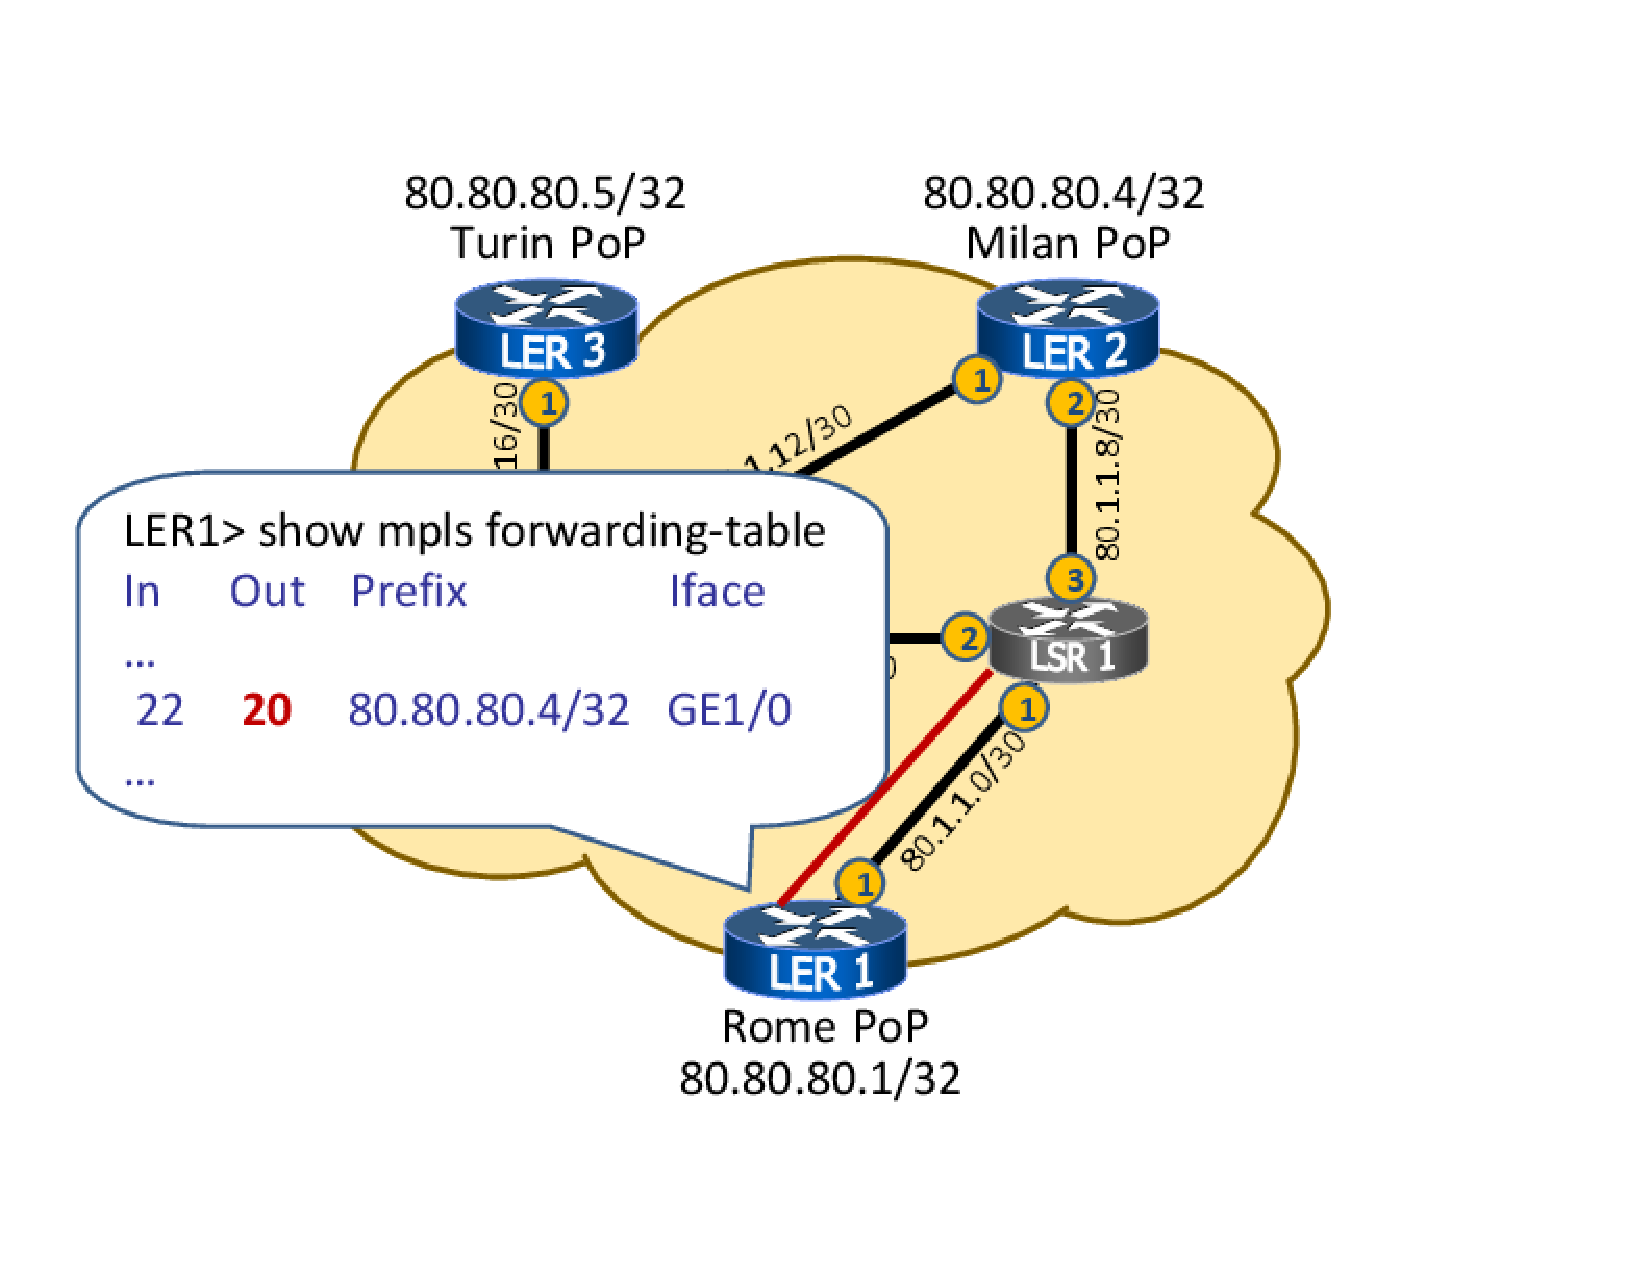
\includegraphics[trim=0cm 1.5cm 0cm 1.5cm, clip=true, width=0.7\columnwidth]{figures/mpls-slides-14}
 \caption{The MPLS forwarding table of LER1.}
 \label{fig:mpls-slides-14}
\end{figure}

\begin{figure}
\centering
 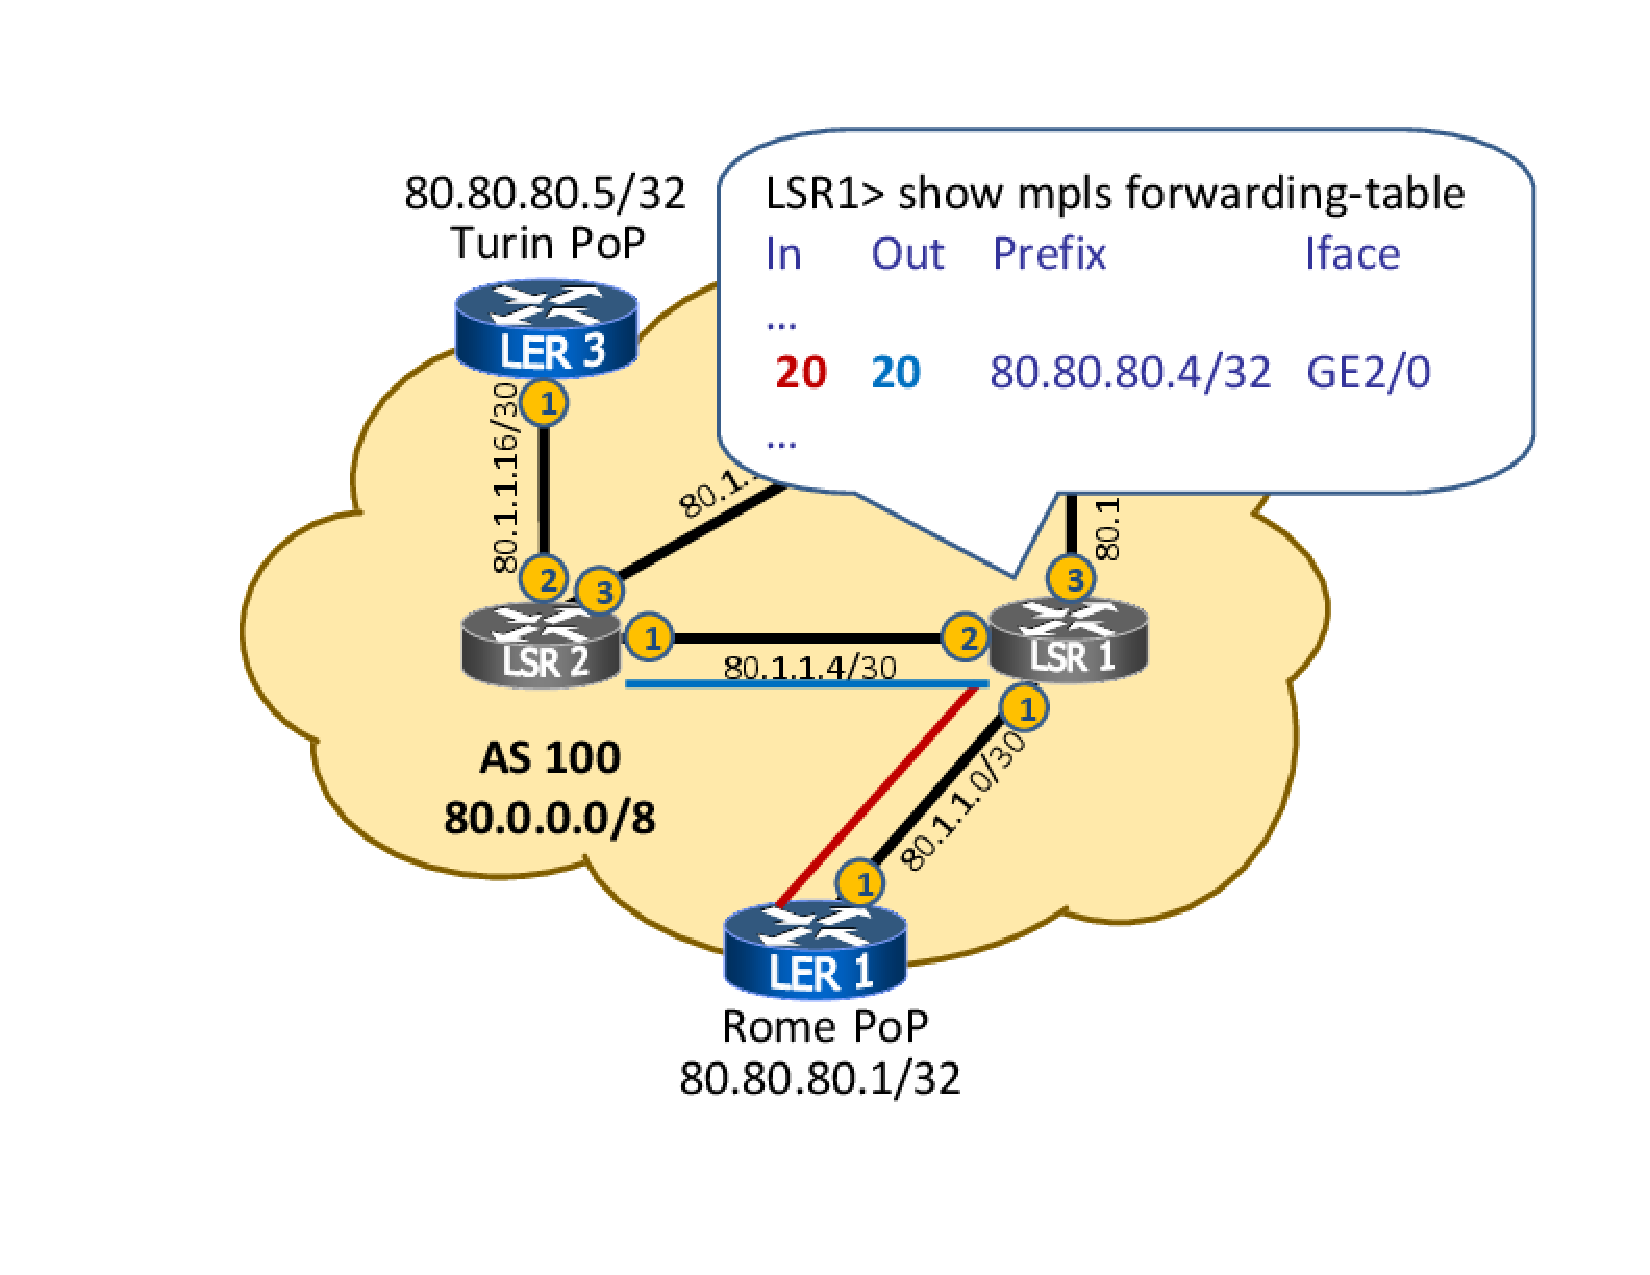
\includegraphics[trim=0cm 1.5cm 0cm 1.5cm, clip=true, width=0.7\columnwidth]{figures/mpls-slides-15}
 \caption{The MPLS forwarding table of LSR1.}
 \label{fig:mpls-slides-15}
\end{figure}

\begin{figure}
\centering
 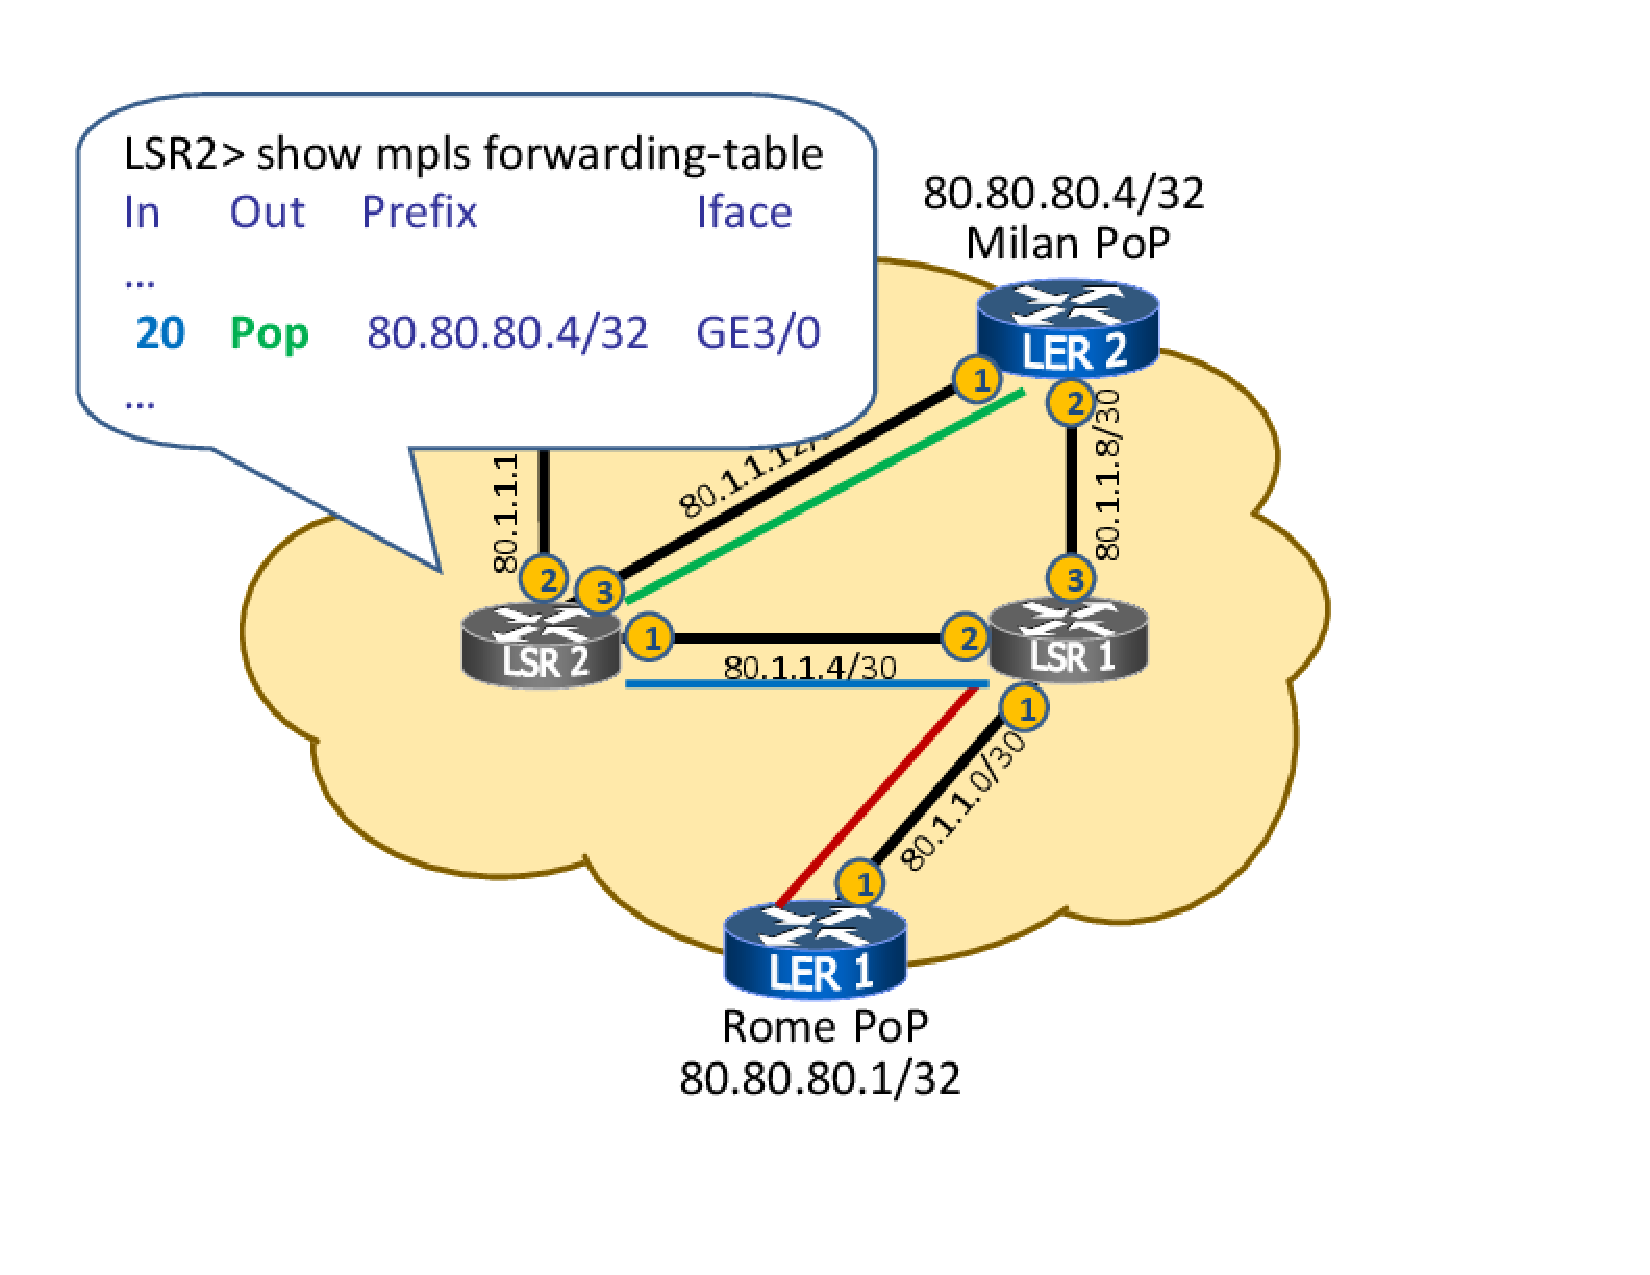
\includegraphics[trim=0cm 1.5cm 0cm 1.5cm, clip=true, width=0.7\columnwidth]{figures/mpls-slides-16}
 \caption{The MPLS forwarding table of LSR2.}
 \label{fig:mpls-slides-16}
\end{figure}

\begin{shaded}
\noindent
Figs.~\ref{fig:mpls-slides-14}, \ref{fig:mpls-slides-15}, and \ref{fig:mpls-slides-16}
show the MPLS forwarding tables of some routers of our network.
\end{shaded}

\begin{figure}
\centering
 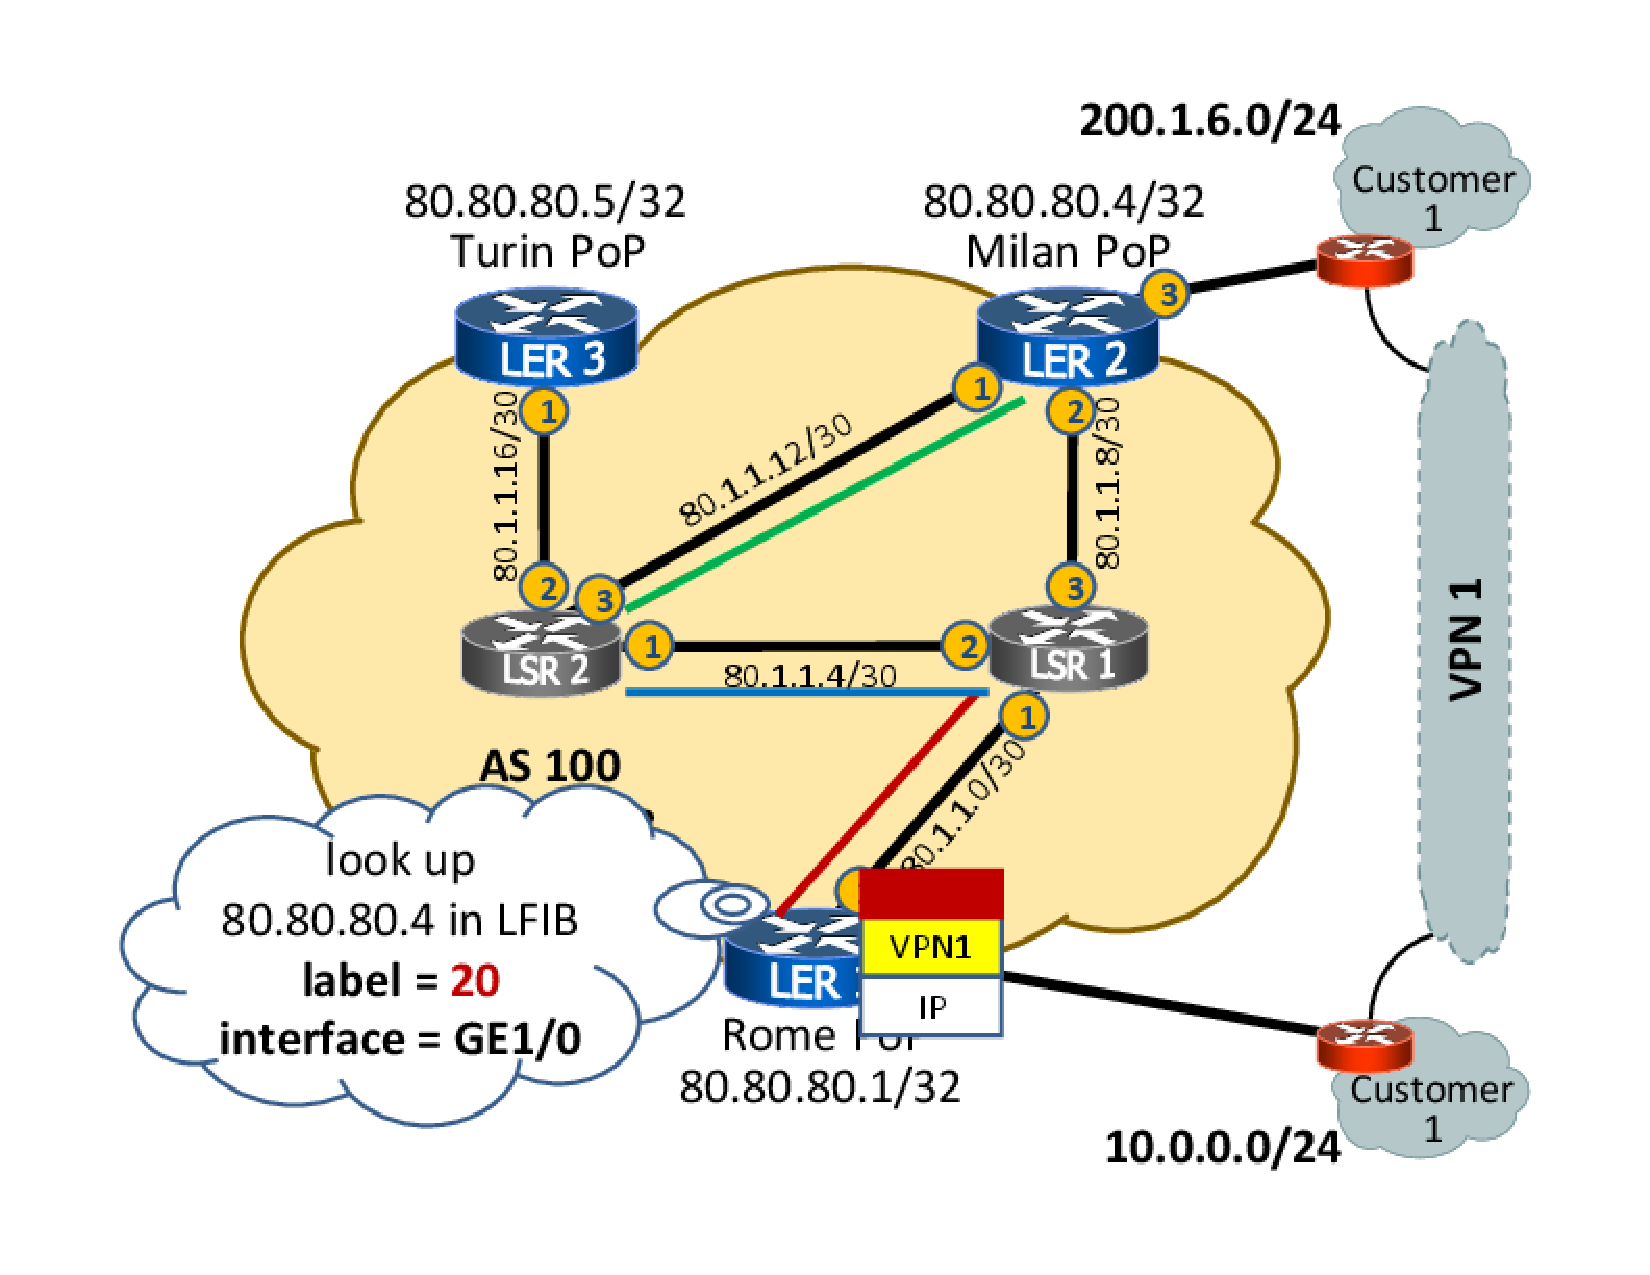
\includegraphics[trim=0cm 1.5cm 0cm 1.5cm, clip=true, width=0.7\columnwidth]{figures/mpls-slides-19}
 \caption{An IP packet originated by the Rome site of Customer 1 reaches PE 
router LER1.}
 \label{fig:mpls-slides-19}
\end{figure}

\begin{figure}
\centering
 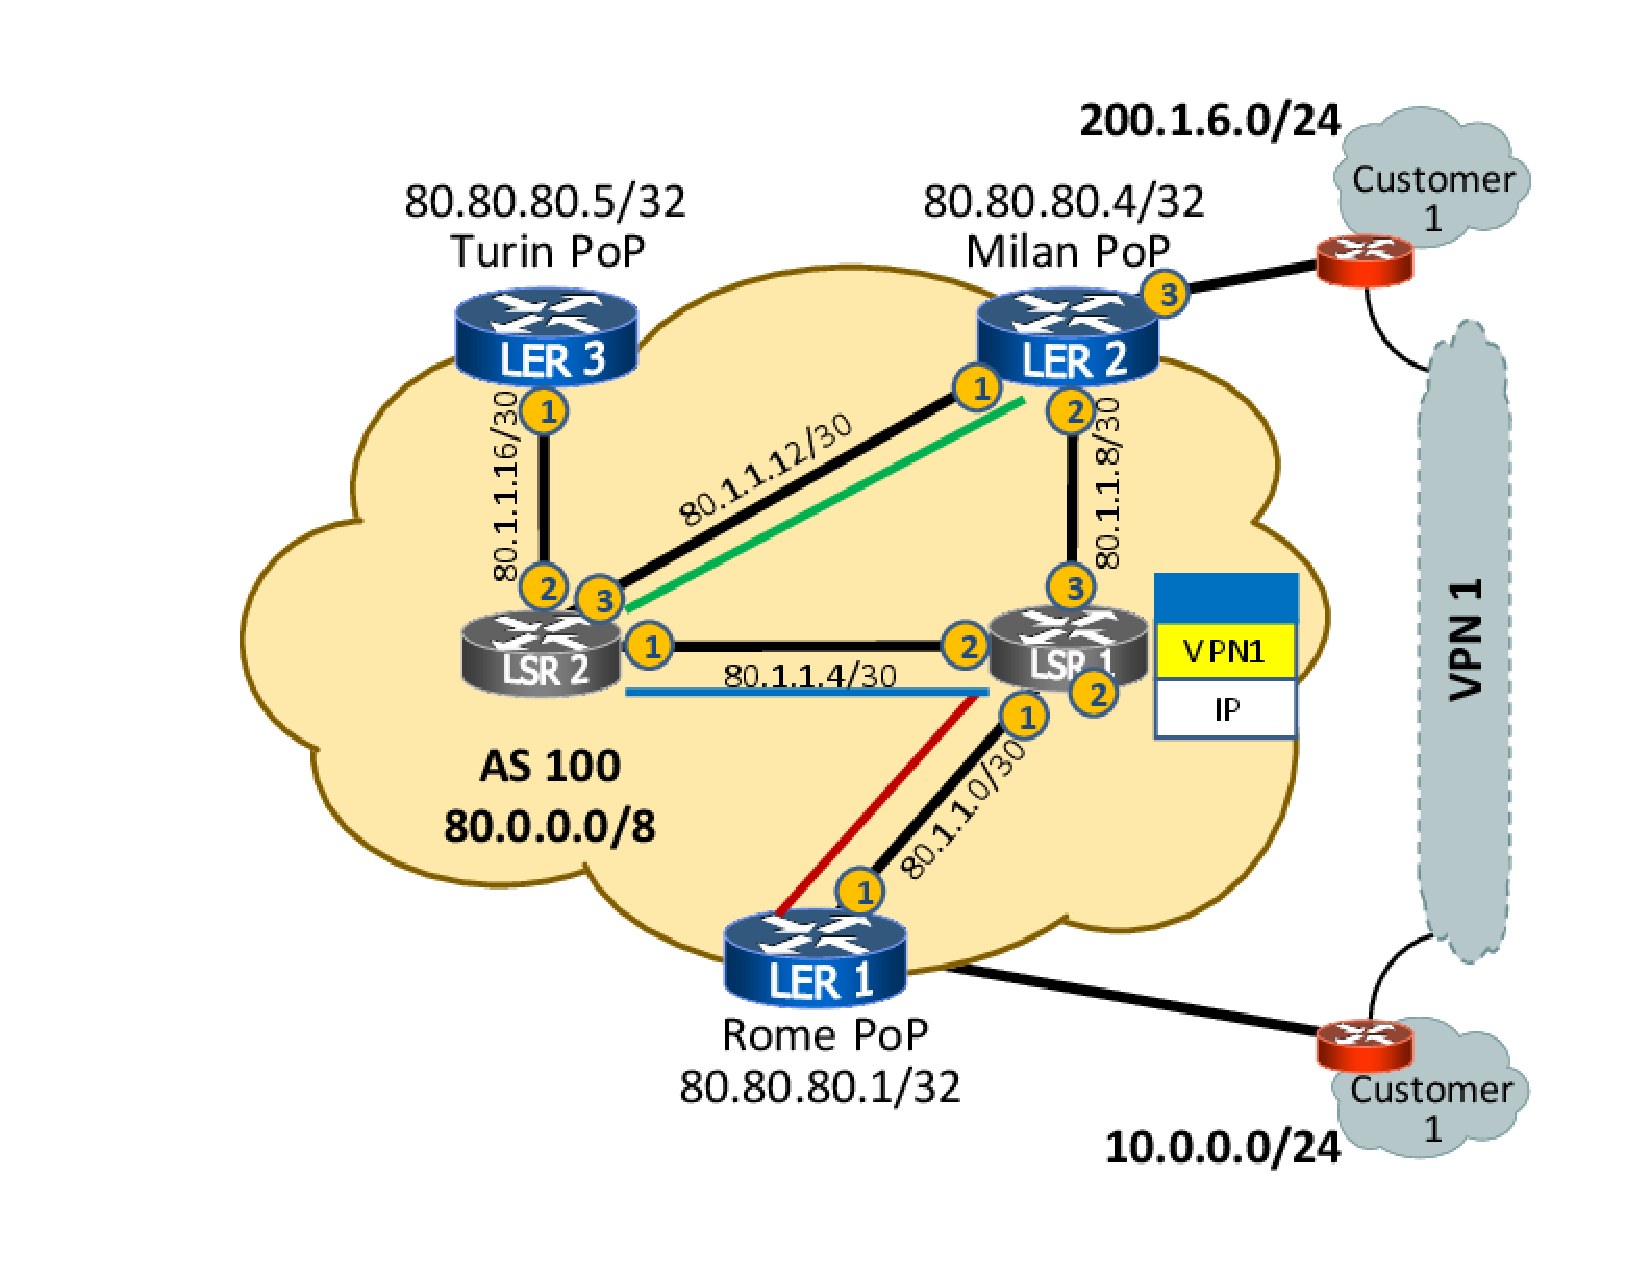
\includegraphics[trim=0cm 1.5cm 0cm 1.5cm, clip=true, width=0.7\columnwidth]{figures/mpls-slides-20}
 \caption{An MPLS packet reaches P router LSR1.}
 \label{fig:mpls-slides-20}
\end{figure}

\begin{figure}
\centering
 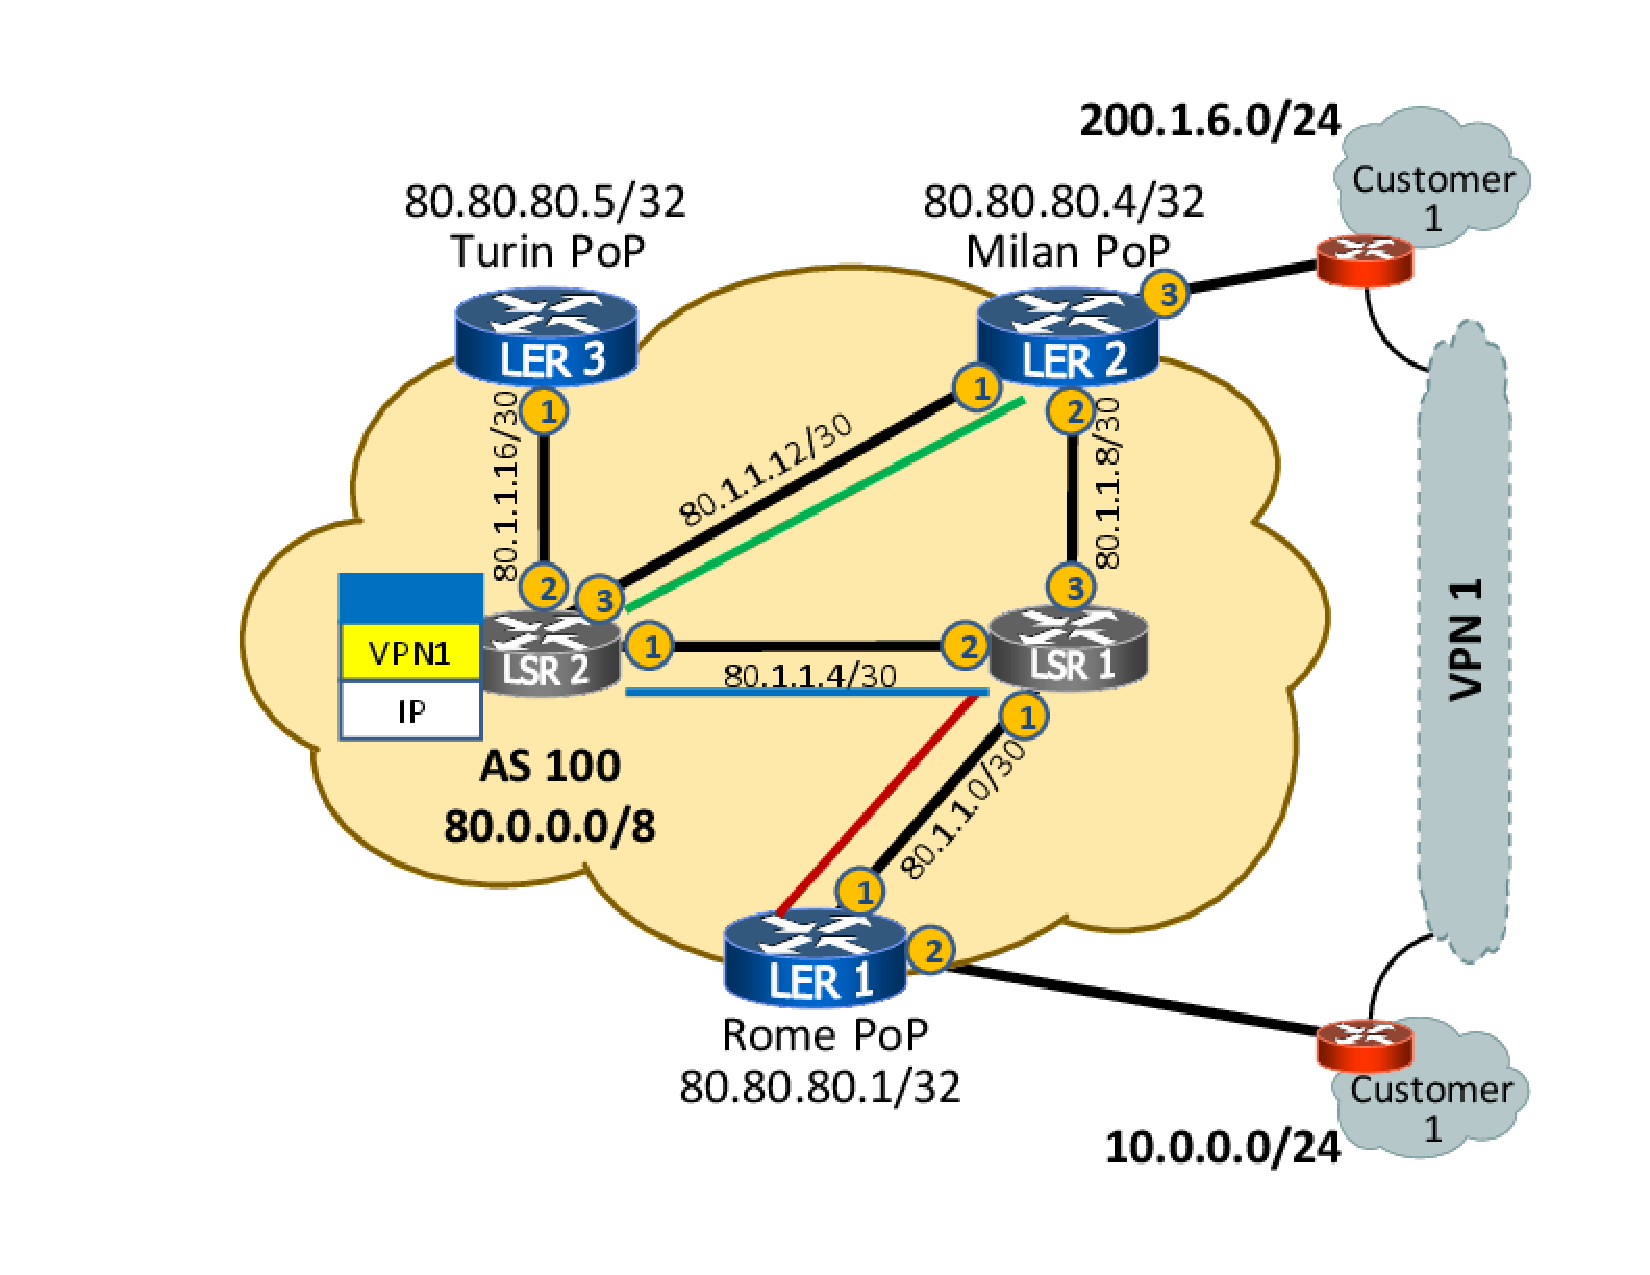
\includegraphics[trim=0cm 1.5cm 0cm 1.5cm, clip=true, width=0.7\columnwidth]{figures/mpls-slides-21}
 \caption{An MPLS packet reaches P router LSR2.}
 \label{fig:mpls-slides-21}
\end{figure}

\begin{figure}
\centering
 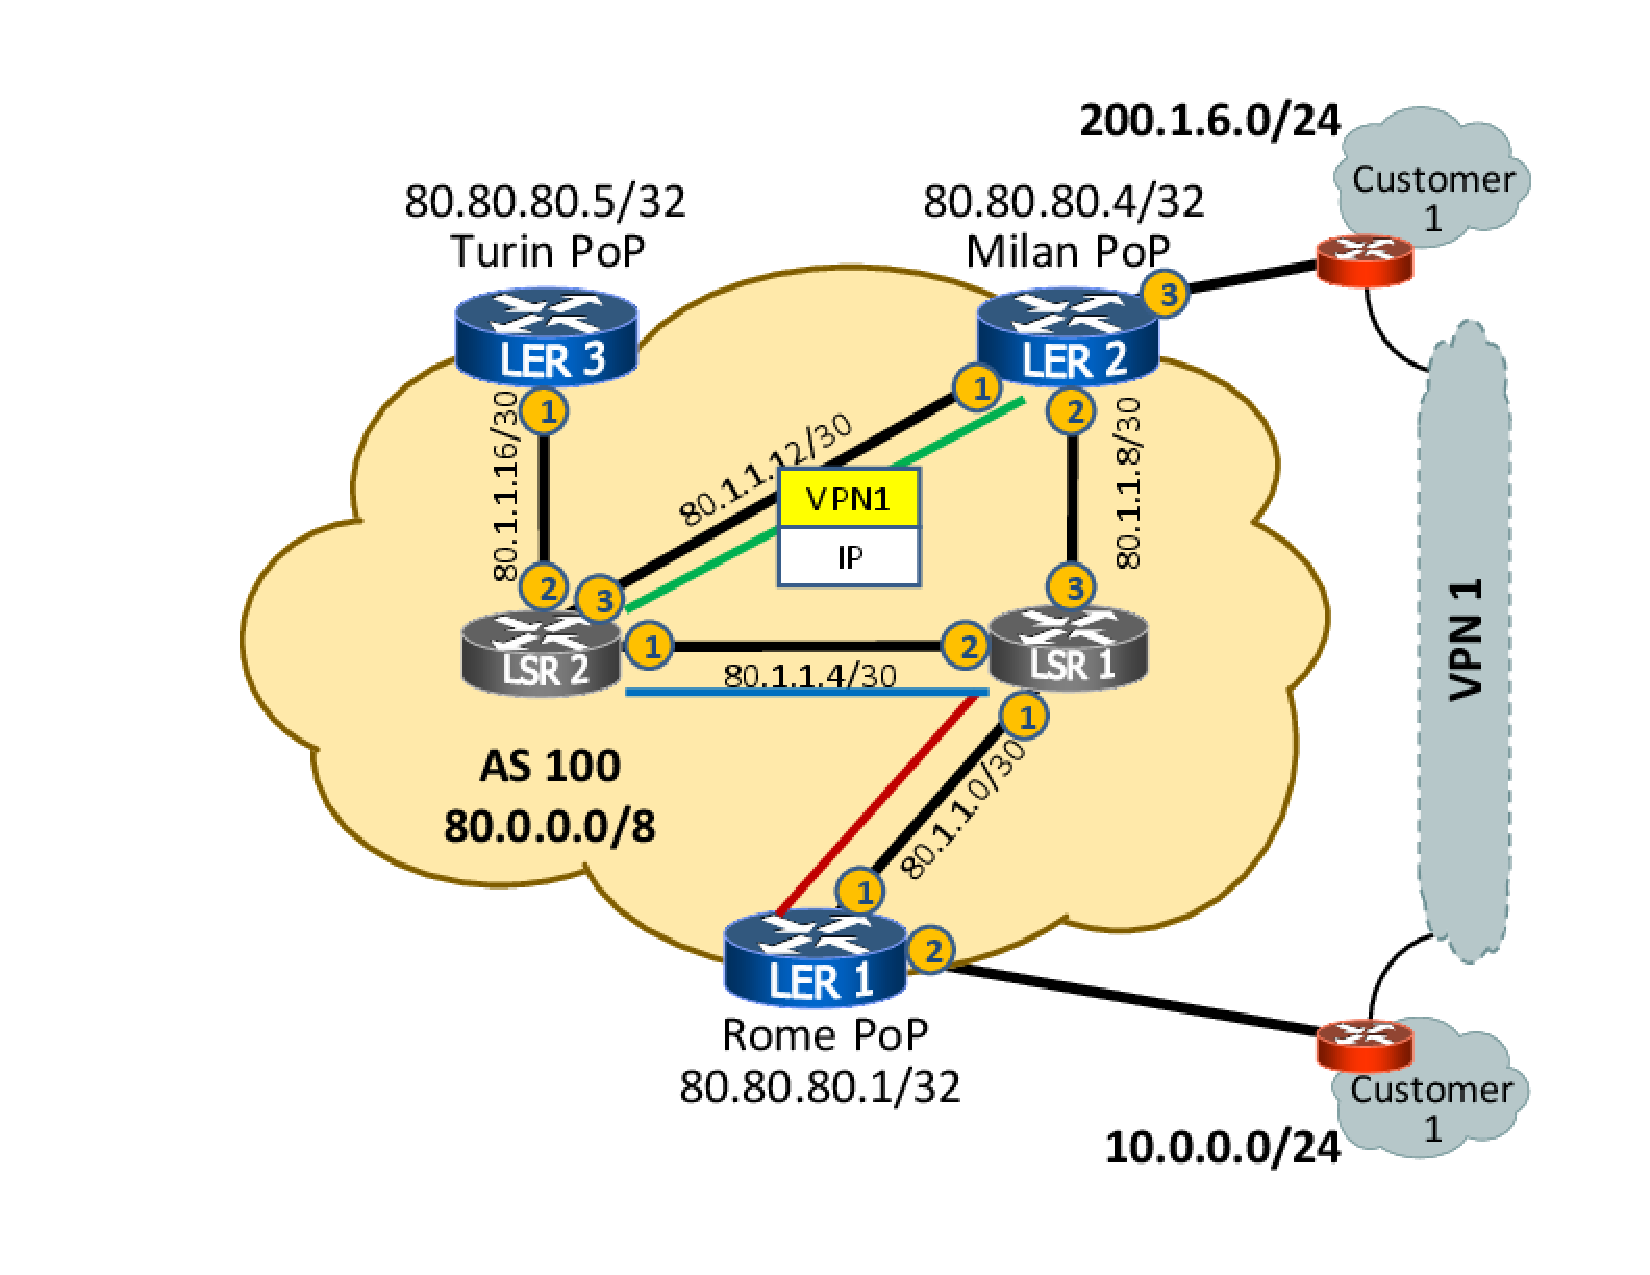
\includegraphics[trim=0cm 1.5cm 0cm 1.5cm, clip=true, width=0.7\columnwidth]{figures/mpls-slides-22}
 \caption{An MPLS packet traveling to PE router LER2.}
 \label{fig:mpls-slides-22}
\end{figure}

\begin{figure}
\centering
 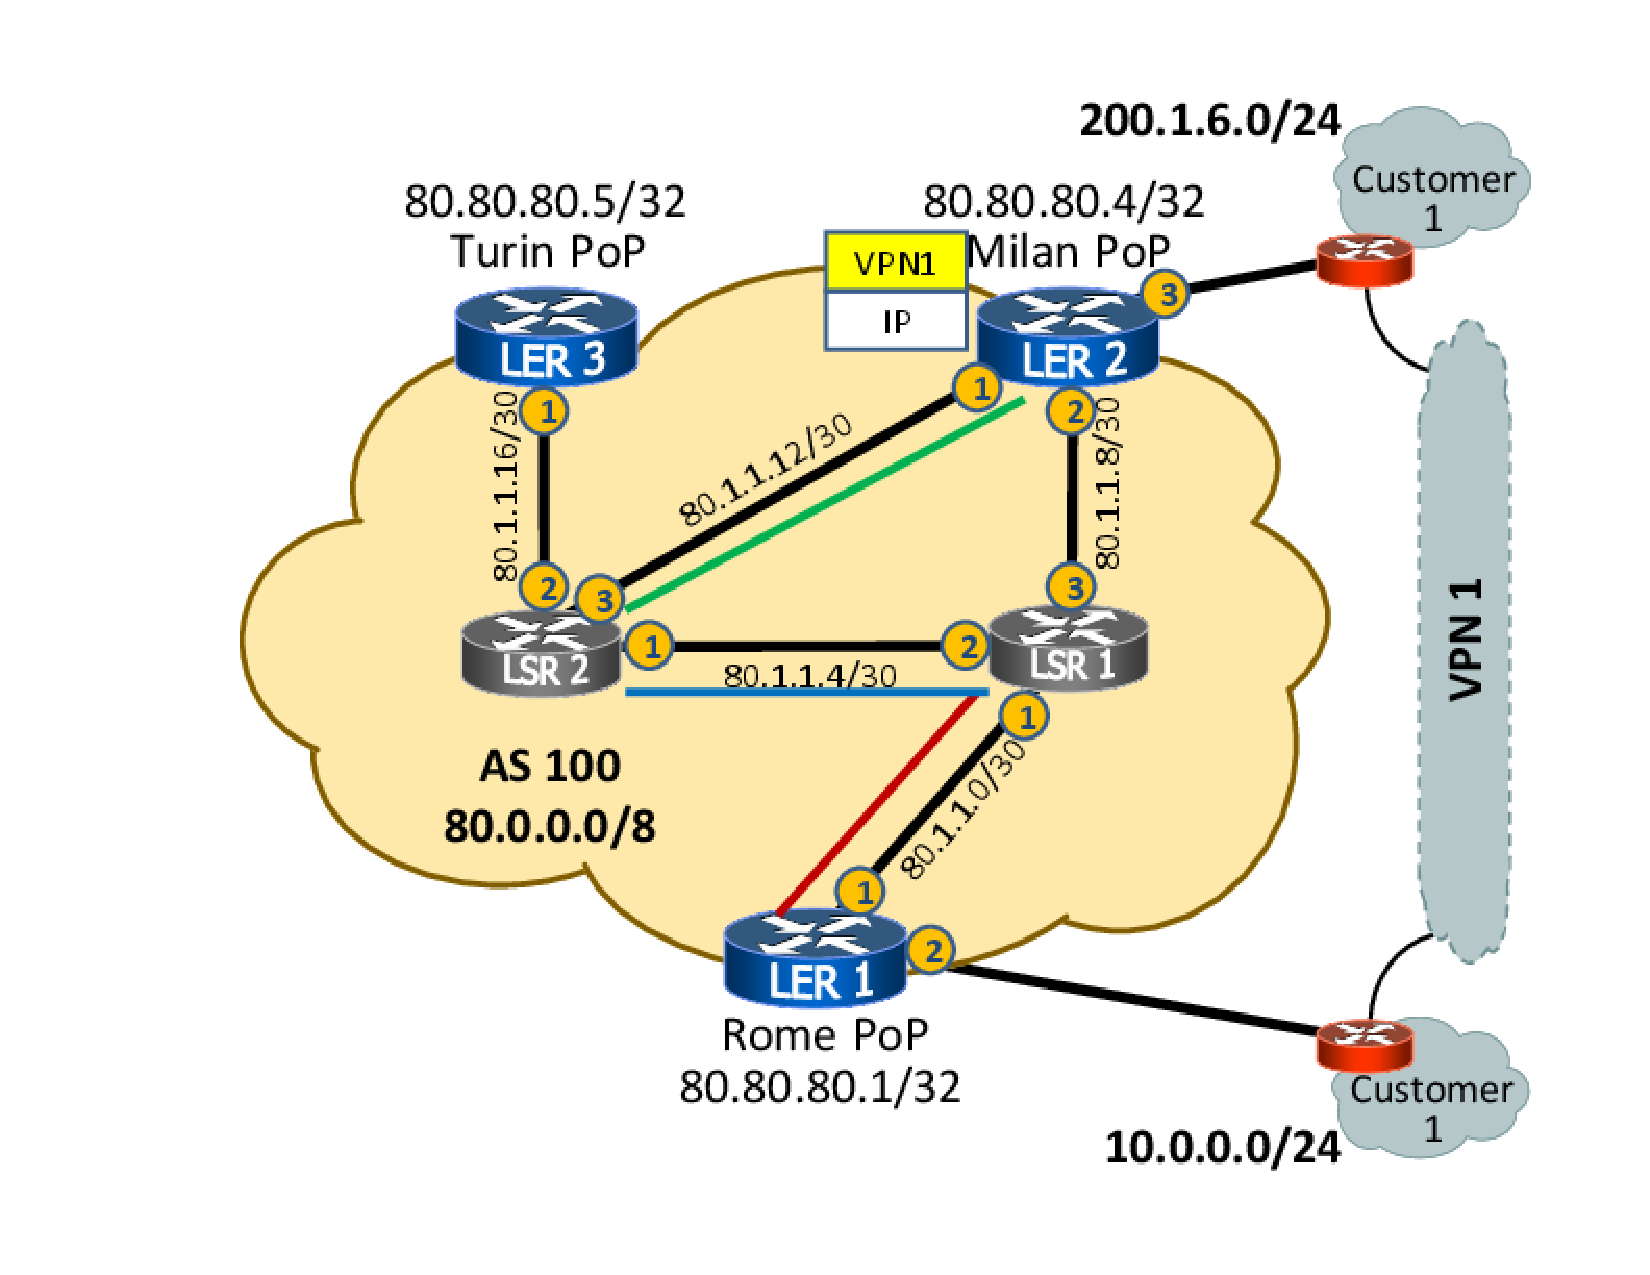
\includegraphics[trim=0cm 1.5cm 0cm 1.5cm, clip=true, width=0.7\columnwidth]{figures/mpls-slides-23}
 \caption{An MPLS packet reaches PE router LER2.}
 \label{fig:mpls-slides-23}
\end{figure}

\begin{figure}
\centering
 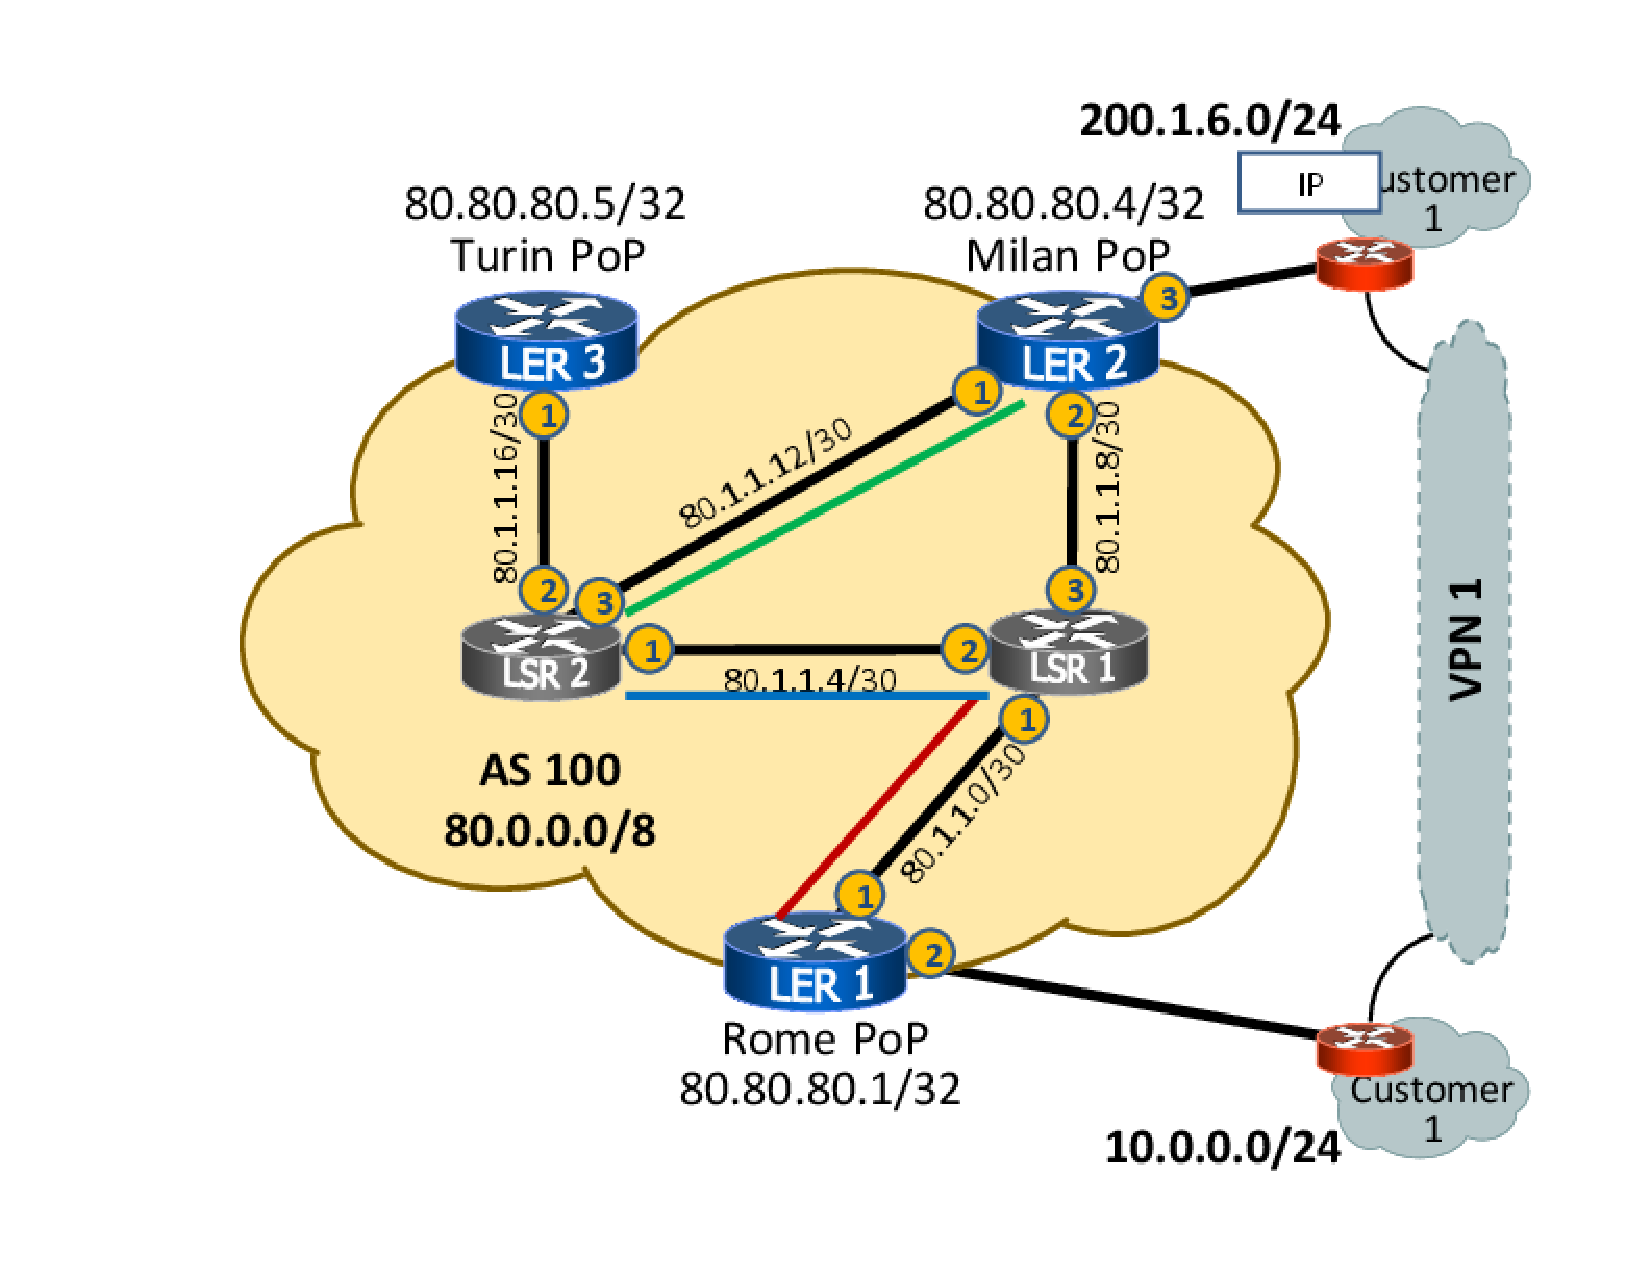
\includegraphics[trim=0cm 1.5cm 0cm 1.5cm, clip=true, width=0.7\columnwidth]{figures/mpls-slides-24}
 \caption{An IP packet for Customer 1.}
 \label{fig:mpls-slides-24}
\end{figure}

\begin{shaded}
\noindent
Figs.~\ref{fig:mpls-slides-19}--\ref{fig:mpls-slides-24} illustrate the travel of a
packet through our network.

First, Fig.~\ref{fig:mpls-slides-19} shows what happens when an IP packet 
originated by the Rome site of Customer 1 reaches the PE called LER1. Namely, it 
is encapsulated into an MPLS packet with two labels and then sent to LSR1. The 
inner label (yellow) identifies the VRF while the outer label (red) is the label 
used for the forwarding process.

Second (Fig.~\ref{fig:mpls-slides-20}), the MPLS packet reaches LSR1, its outer 
red label is replaced with a blue label, and the packet is forwarded to LSR2.

Third (Figs.~\ref{fig:mpls-slides-21} and~\ref{fig:mpls-slides-22}), the MPLS 
packet reaches LSR2. LDP makes LSR2 aware that it is the penultimate hop in the 
LSP. For this reason, LSR2 simply pops the outer label and forwards the packet 
to LER2.

Fourth (Fig.~\ref{fig:mpls-slides-23}), the MPLS packet reaches LER2. LER2 
notices that there is only one MPLS label (which used to be the inner label), so 
the packet is meant to be forwarded via IP in one of the VPNs that LER2 serves. 
LER2 uses the VRF label to identify the VRF instance, then looks up the IP 
destination address in the VRF forwarding table.

Fifth (Fig.~\ref{fig:mpls-slides-24}), the IP packet is delivered to its final
destination.
\end{shaded}




%%%%%%%%%
%%%%%%%%%
%%%%%%%%%
%%%%%%%%%
%%%%%%%%%
\section{Advanced Topics}\label{se:advanced}

In this section we give more technical details about dynamic routing and connecting to the
Internet, creating complex VPN topologies, and dealing with IP-specific 
features (e.g., MTU) that need extra care when encapsulation is involved.

%
%%%
%%%%%
%%%
%
\subsection{Dynamic Routing and Connecting to the Internet}\label{sse:internet}

So far we have not yet discussed how the PE router can learn the prefixes that 
are served by its directly attached CE router. Of course, it is trivial to 
configure static routes on the PE, however this creates an undesirable 
coupling between the provider and the customer: whenever the customer wants to 
add a different IP subnet, it has to bother the provider to configure static 
routes before that IP subnet is reachable from other customer sites in the same 
VPN.

The solution is to have the CE and the PE establish an eBGP peering where the CE 
announces its local networks, while the PE announces all the networks that it 
learns in the same VPN. Observe that the, contrary to the MP-BGP peerings among 
PEs, peerings between CEs and PEs are pure eBGP peering: the CE does not know 
anything about VPNs and route distinguishers. It is the MP-BGP process on the PE 
router that takes care of processing the reachability information learned from 
the CE and updating the VPN reachability information accordingly.

Setting up an eBGP session in order to use the MPLS-VPN service may discourage 
those customers who do not have a strong BGP expertise. In such cases, usually 
the providers also offer to their customers CE management and configuration.

A BGP peering between the CE and the PE also allows a CE in a VPN to announce a 
default route, causing all other sites in the same VPN to route Internet traffic 
via that CE router. This might be advantageous if the customer's policy forces 
Internet traffic to pass through a centralized checkpoint (e.g., a firewall or a 
proxy). However, this is not the only way to connect a VPN to the Internet. For 
example, a PE might be configured to forward natively all the packets from a CE 
which do not match any VPN route. Alternatively, the default route might be 
given its own route target, and whenever a VPN site needs Internet access the PE 
simply imports that route target in the corresponding VPN routing table. We 
refer the reader to~\cite{rfc4364} for a discussion of alternatives to get 
Internet access within a VPN.

\begin{shaded}
In our sample network, customer 1 would like to be able to create a new IP 
subnet in Rome, advertise the new subnet to LER1 via an eBGP peering, and 
automatically make the customer site in Milan able to access it. LER1 should 
receive the new route via eBGP, tag the route with the correct RD value, and 
advertise it in MP-BGP. In order to do this, it suffices to configure an eBGP 
peering in the context of a VRF instance, as the following configuration snippet 
of LER1 shows.

\begin{codice}
\begin{verbatim}
router bgp 100
  address-family ipv4 vrf VPN1
  neighbor 10.0.0.2 remote-as 65001
  exit-address-family
  !
  address-family ipv4 vrf VPN2
  neighbor 193.1.1.2 remote-as 65002
  exit-address-family 
\end{verbatim}
\end{codice}


\end{shaded}



%
%%%
%%%%%
%%%
%
\subsection{Designing Complex VPNs}
So far we have assumed any-to-any connectivity within a VPN, i.e., all sites of 
a VPN communicate with all other sites. Sometimes more sophisticated 
configurations are needed. For example we might have a VPN where not all pairs 
of sites are allowed to exchange packets. A typical situation is the so called 
hub-and-spoke configuration, where a customer has a main site and several 
peripheral sites and the peripheral sites can communicate only through the main 
site.

How to do this is illustrated in the following example.

\begin{figure}
\centering
 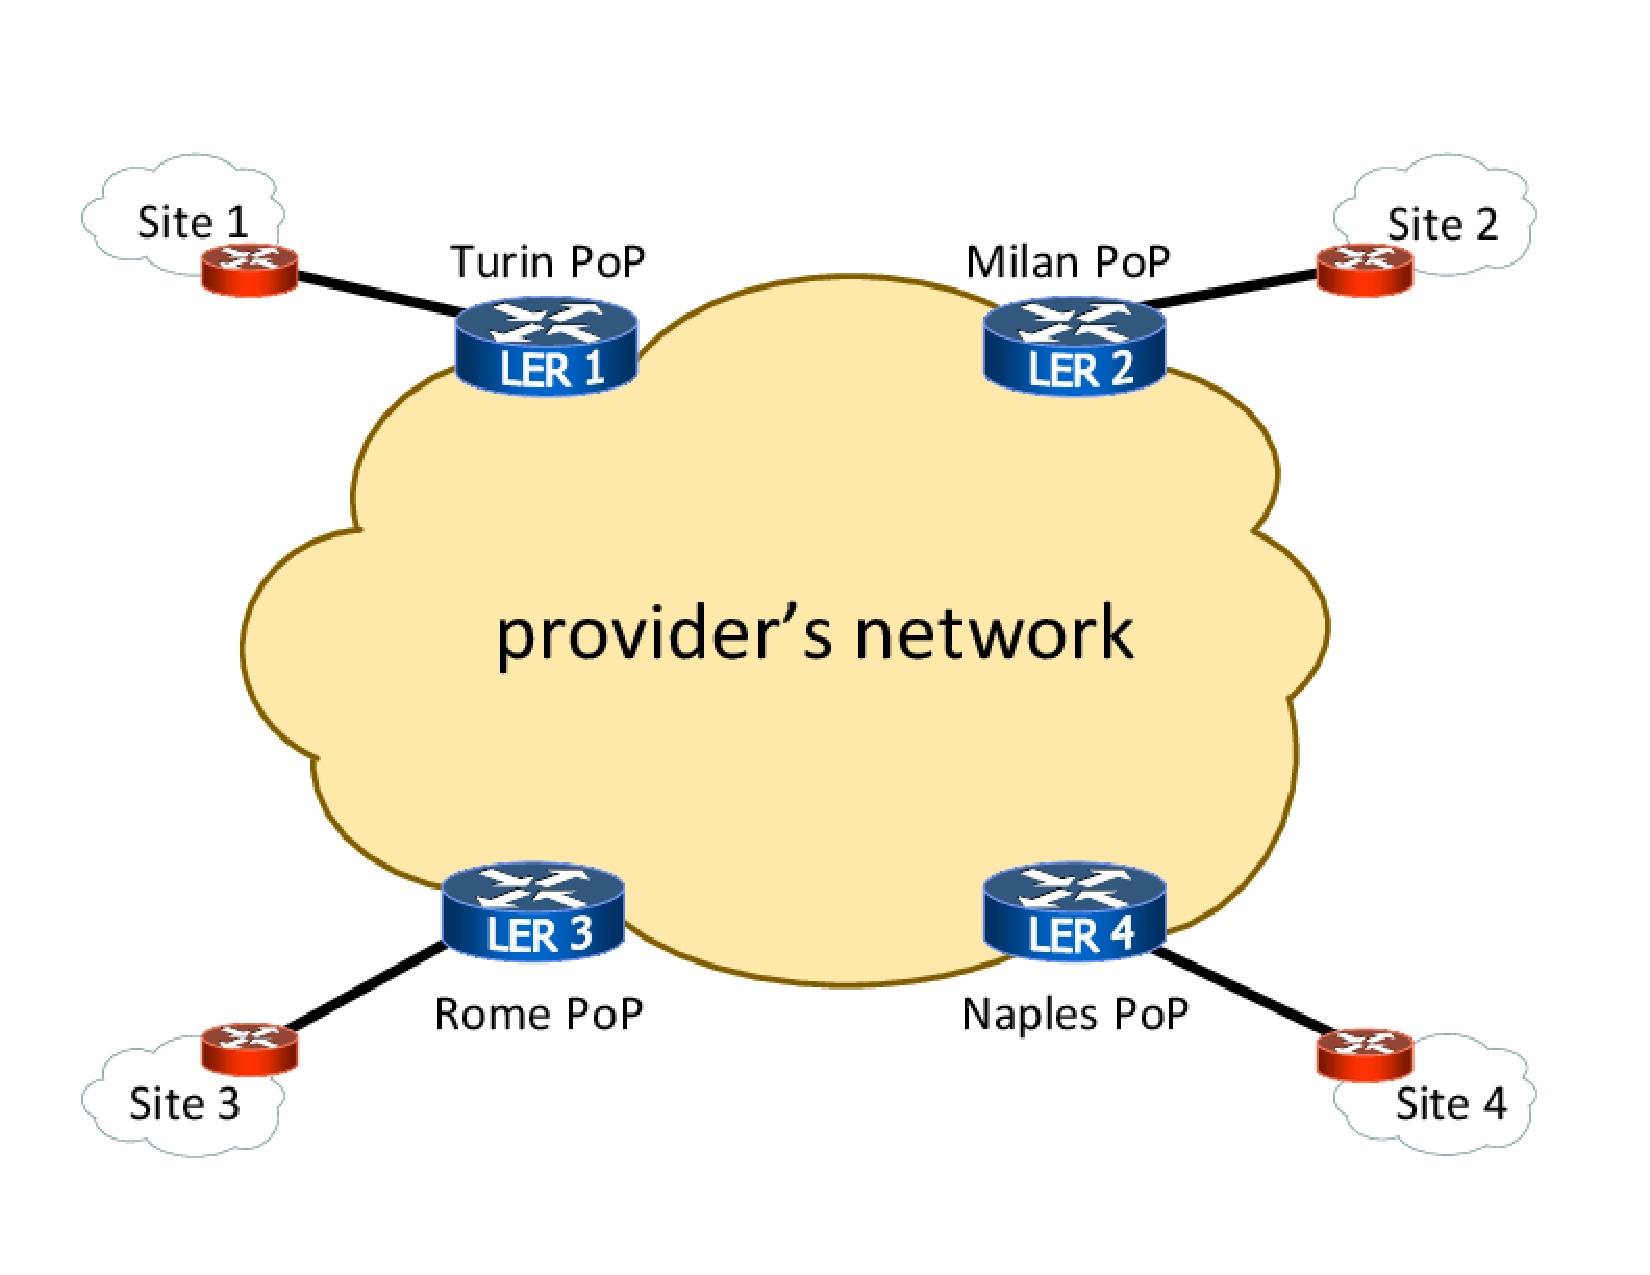
\includegraphics[trim=0cm 1.5cm 0cm 1.5cm, clip=true, width=0.7\columnwidth]{figures/mpls-slides-27}
 \caption{A configuration where a single customer has four sites: Site 2, 3, and 4 are
only allowed to exchange traffic with  Site 1 in Rome.}
 \label{fig:mpls-slides-27}
\end{figure}

\begin{shaded}
\noindent
A suitable use of Route Distinguishers and Route Targets allows sophisticated
configurations like the one shown in Fig.~\ref{fig:mpls-slides-27} where Rome is
the main site and Turin, Milan, and Naples are the peripheral sites.


%Suppose we choose the following Route Distinguishers for the four sites, where Rome is
%the main site and Turin, Milan, and Naples are the peripheral sites:
%\begin{enumerate}
%\item[Turin:] RD \texttt{100:1}
%\item[Milan:] RD \texttt{100:2}
%\item[Rome:] RD \texttt{100:3}
%\item[Naples:] RD \texttt{100:4}
%\end{enumerate}

We can choose  Route Distinguisher \texttt{100:1} for all four sites and split the customer VPN into three VPNs. VPN1 is used to connect Turin with Rome,
VPN2 is used to connect Milan with Rome, and VPN3 is used to connect Naples with Rome.

For each VPN we define a distinct Route Target:
\begin{enumerate}
\item[VPN1:] \texttt{100:1000}
\item[VPN2:] \texttt{100:2000}
\item[VPN3:] \texttt{100:3000}
\end{enumerate}

The configuration of peripheral sites, like for example Turin, is as
follows:\\
\begin{codice}
\begin{verbatim}
ip vrf siteTurin
        rd 100:1
        route-target import 100:1000
        route target export 100:1000
\end{verbatim}
\end{codice}

Rome's PE configuration (the hub) is as follows:\\
\begin{codice}
\begin{verbatim}
ip vrf siteRome
        rd 100:1
        route-target import 100:1000
        route target export 100:1000
        route-target import 100:2000
        route target export 100:2000
        route-target import 100:3000
        route target export 100:3000
\end{verbatim}
\end{codice}

In this way Rome imports all the Route Targets and exports all the Route Targets and is
hence able to communicate with all sites. On the other hand a peripheral site like Turin
imports and exports Route targets only with respect to Rome and hence is able to communicate 
with Rome only.
\end{shaded}



%
%%%
%%%%%
%%%
%
\subsection{ToS, TTL, and MTU}
Whenever encapsulation of IP packets happens, there are three main questions 
that arise:
\begin{enumerate}
 \item what happens to the ToS / DSCP information in the IP header that the 
customer might have set in order to properly prioritize traffic?
 \item what happens to the TTL field in the IP header and how does 
encapsulation cope with forwarding loops?
 \item how does encapsulation affect MTU for upper layer protocols?
\end{enumerate}

Luckily, MPLS has an easy answer for the first two questions. Recall from 
Fig.~\ref{fig:mpls-header} that MPLS has dedicated fields for ToS and TTL. When 
the ingress PE router receives an IP packet from the CE router, it simply copies 
the values of ToS and of TTL in the MPLS header. More precisely, a push operation 
implies copying ToS and TTL from the IP header to the MPLS header. Conversely, a 
pop operation implies copying the TTL value from the MPLS header back to the IP 
header. This way, the TTL continues to serve as a hop count%
% 
\footnote{Observe that when the TTL in the MPLS header reaches $0$ (e.g. in a 
traceroute), a P router does not know how to send the corresponding ICMP error 
back to the sender, because it lacks information about VPNs. A naive yet 
effective solution is to generate the ICMP packet and label-switch it to the 
egress PE anyway. The egress PE (which has information about VPNs) will then 
send the ICMP packet back to the sender.} 
% 
even within the MPLS network, and P routers can honor the quality of service 
parameters related to the ToS field.

Regarding the third question, since an MPLS label takes 4 bytes and the PE 
router pushes two of them, the MTU within the MPLS network should be at least 8 
bytes larger than the MTU that the CE is aware of. Given that modern OSes tend 
to perform path MTU discovery by default, MTU is becoming less of an issue for 
MPLS deployments. Rewriting the Maximum Segment Size TCP options at the PE router is also a 
common solution, even though it does not support UDP traffic.


%%%%%%%%%
%%%%%%%%%
%%%%%%%%%
%%%%%%%%%
%%%%%%%%%
\section{Summary}\label{sec:summary}

\subsection{Strengths of MPLS VPNs}

After having described the details of MPLS VPNs, we are able to discuss the 
extent to which the goals that we stated in Section~\ref{sec:intro-goals} are 
met.

By using Route Distinguishers and label stacks within the provider cloud, 
customers can retain their IP address plan and the traffic belonging to 
different customers is properly segregated. Moreover, the configuration of CE 
routers is completely unaware of MPLS-specific details. Since MPLS transports 
QoS information by copying the ToS field from the IP header, MPLS VPNs can in 
principle provide different forwarding treatment to different packets. However, 
the architecture of MPLS VPNs does not inherently support QoS, because LSPs are 
simply built from the underlying IP plane. Other mechanisms (e.g., 
\cite{rfc3209}) can be employed to compute LSPs based on QoS features. 

Providers are able to keep the configuration in the core of the network 
extremely simple and scalable: in fact, the configuration of P routers does not 
depend on the number of deployed VPNs. Since the backbone is only concerned with 
transporting packets from a PE to another, the sizeof the forwarding table of P routers only depends on the number of PEs and does not depend on the number of prefixes of VPNs.
%forwarding table of P routers only contains one entry for each loopback address, which makes forwarding performance independent of the number of VPNs. 
Configuring a new VPN implies 
modifying the configuration of the PE routers that are directly connected to the 
customer's sites. Moreover, such a configuration boils down to assigning a 
unique RD and RT and establishing eBGP peerings with the CE routers.

%%%%%%%
%%%%%%%
%%%%%%%
\subsection{Limitations of MPLS VPNs}


Virtual Private Networks designed with MPLS have also some known limitations. 
At least the following should be mentioned.

\begin{itemize}

 \item BGP know-how is needed to configure the customer CE. As discussed in Section~\ref{sse:internet}, this sometimes forces the carrier to provide also CE management. 

 \item Customer CEs need to support BGP if eBGP peering are established with the PEs. This may not be the case for cheap entry-level router models. As an alternative, BGP can be replaced by static routes configured on PEs, sacrificing part of the flexibility that a dynamic routing protocol between CEs and PEs provides.

 \item The P in the MPLS acronym stands for ``Private''. However, MPLS VPNs are only private at routing level: no authentication, confidentiality, or integrity is provided by the architecture. For instance, the provider can inspect all customers' traffic in plaintext. Even worse, since the separation is enforced at the routing level, it turns out that the ability of guaranteeing isolation within the same VPN actually depends on the provider's topology~\cite{integrity}.

 \item The basic MPLS architecture lacks support for quality of service. QoS can usually be offered on top of MPLS, e.g., by establishing LSPs which reflect traffic engineering policies. However, adding traffic engineering and quality of service support comes at the cost of keeping more state in the network, hence posing scalability concerns~\cite{juniper-preso,rfc5439}.

 \item In most configurations, the customer and the provider share the job of maintaining a network, which potentially complicates debugging routing and connectivity problems.

\end{itemize}


%%%%%%%
%%%%%%%
%%%%%%%
\subsection{Further Readings}\label{sec:further-readings}

The interested reader could refer to the classical books about MPLS authored by Minei and Lucek~\cite{minei-lucek} and by De Ghein~\cite{de-ghein}.

Most of the technologies regarding MPLS are defined by RFCs. These include the main MPLS VPNs architecture~\cite{rfc3031,rfc4110}, label distribution via LDP~\cite{rfc5036}, Layer 2 VPNs~\cite{rfc4664}, BGP variants~\cite{rfc2858,rfc4364,rfc5512}, and RSVP-TE~\cite{rfc3209}.

Considerations about about MPLS VPNs integrity and scalability can be found in~\cite{integrity} and~\cite{juniper-preso,rfc5439}, respectively.


\subsection*{Acknowledgments}

We thank the anonymous reviewers for constructive criticism and for suggestions 
that helped us improve both the content and the presentation of this chapter. We 
also thank Mario Cola and Massimo Rimondini for their help and 
friendship.


\bibliographystyle{plain}
\bibliography{bibliography}

\end{document}


